% This file was created (at least in part) by the script ParseMdtoLatex by Louis du Plessis
% (Available from https://github.com/taming-the-beast)

\documentclass[11pt]{article}
%%%%%%%%%%%%%%%%%%%%%%%%%%%%%%%%%%%%%%%%%%%%%%%%%%%%%%%%%%%%%%%
% DO NOT EDIT THIS FILE UNLESS YOU KNOW WHAT YOU ARE DOING!!! %
%%%%%%%%%%%%%%%%%%%%%%%%%%%%%%%%%%%%%%%%%%%%%%%%%%%%%%%%%%%%%%%

\usepackage[]{authblk}
\usepackage{graphicx}
\usepackage{color}
\usepackage{longtable}
\usepackage{hanging}
\usepackage{indentfirst}
\usepackage{setspace}
\usepackage{enumitem}
\usepackage{verbatim}
\usepackage{upgreek}
\usepackage{framed}
\usepackage{textcomp}
\usepackage{url}
\usepackage{soul}
\usepackage{amsmath, amsfonts,amssymb,mathrsfs}
\usepackage{fancyhdr}
\usepackage[compact]{titlesec}
\usepackage[T1]{fontenc}
\usepackage{lmodern}

\usepackage[backend=bibtex,hyperref=true,citestyle=authoryear,bibstyle=authortitle,firstinits=true,terseinits=true,doi=false,url=false,eprint=false,maxbibnames=10,maxcitenames=2]{biblatex}
\DeclareCiteCommand{\cite}
  {\usebibmacro{prenote}}
  {\usebibmacro{citeindex}%
   \printtext[bibhyperref]{\usebibmacro{cite}}}
  {\multicitedelim}
  {\usebibmacro{postnote}}

\DeclareCiteCommand*{\cite}
  {\usebibmacro{prenote}}
  {\usebibmacro{citeindex}%
   \printtext[bibhyperref]{\usebibmacro{citeyear}}}
  {\multicitedelim}
  {\usebibmacro{postnote}}

\DeclareCiteCommand{\parencite}[\mkbibparens]
  {\usebibmacro{prenote}}
  {\usebibmacro{citeindex}%
    \printtext[bibhyperref]{\usebibmacro{cite}}}
  {\multicitedelim}
  {\usebibmacro{postnote}}

\DeclareCiteCommand*{\parencite}[\mkbibparens]
  {\usebibmacro{prenote}}
  {\usebibmacro{citeindex}%
    \printtext[bibhyperref]{\usebibmacro{citeyear}}}
  {\multicitedelim}
  {\usebibmacro{postnote}}

\DeclareCiteCommand{\footcite}[\mkbibfootnote]
  {\usebibmacro{prenote}}
  {\usebibmacro{citeindex}%
  \printtext[bibhyperref]{ \usebibmacro{cite}}}
  {\multicitedelim}
  {\usebibmacro{postnote}}

\DeclareCiteCommand{\footcitetext}[\mkbibfootnotetext]
  {\usebibmacro{prenote}}
  {\usebibmacro{citeindex}%
   \printtext[bibhyperref]{\usebibmacro{cite}}}
  {\multicitedelim}
  {\usebibmacro{postnote}}

\DeclareCiteCommand{\textcite}
  {\boolfalse{cbx:parens}}
  {\usebibmacro{citeindex}%
   \printtext[bibhyperref]{\usebibmacro{textcite}}}
  {\ifbool{cbx:parens}
     {\bibcloseparen\global\boolfalse{cbx:parens}}
     {}%
   \multicitedelim}
  {\usebibmacro{textcite:postnote}}

\newcommand{\citep}{\parencite}
\newcommand{\citet}{\textcite}
\defbibheading{relevref}[\refname]{\section*{Relevant References}}

\renewcommand{\postnotedelim}{\iffieldpages{postnote}{\addcolon}{\addcomma\space}} 
\DeclareFieldFormat{postnote}{#1} 

\DeclareFieldFormat[article, inbook, incollection, inproceedings, patent, thesis, unpublished]{title}{#1}
\DeclareFieldFormat[article, inbook, incollection, inproceedings, patent, thesis, unpublished]{journaltitle}{\mkbibemph{#1}\nopunct}
\DeclareFieldFormat[article, inbook, incollection, inproceedings, patent, thesis, unpublished]{volume}{{#1}\addcolon} %puts volume number in parens
%\DeclareFieldFormat[article, inbook, incollection, inproceedings, patent, thesis, unpublished]{year}{\mkbibparens{#1}\nopunct} %puts year in parens

\DeclareFieldFormat[article, incollection, patent, thesis, unpublished]{pages}{{\nopp#1}}

\DeclareFieldFormat{sentencecase}{\MakeSentenceCase{#1}}

\renewbibmacro*{title}{%
  \ifthenelse{\iffieldundef{title}\AND\iffieldundef{subtitle}}
    {}
    {\ifthenelse{\ifentrytype{article}\OR\ifentrytype{inbook}%
      \OR\ifentrytype{incollection}\OR\ifentrytype{inproceedings}%
      \OR\ifentrytype{inreference}}
      {\printtext[title]{%
        \printfield[sentencecase]{title}%
        \setunit{\subtitlepunct}%
        \printfield[sentencecase]{subtitle}}}%
      {\printtext[title]{%
        \printfield[titlecase]{title}%
        \setunit{\subtitlepunct}%
        \printfield[titlecase]{subtitle}}}%
     \newunit}%
  \printfield{titleaddon}}

\DefineBibliographyStrings{english}{% various adjustments to common bib entry strings
urlseen = {Accessed:},% What goes in front of the date a URL was accessed/retrieved etc.
editor = {(Ed)},%Ed – no dot, in brackets
editors = {(Eds)},% Eds – no dot, in brackets
byeditor = {(Ed.)}}% ‘Edited by’ for edited works

\DeclareNameAlias{default}{last-first}

\renewbibmacro{in:}{}

\renewbibmacro{publisher+location+date}{
  \iflistundef{publisher}
    {}
    {\printlist{publisher}%
       {\addcomma\space}%
      \iflistundef{location}
        {}
        {\printlist{location}}%
    }
}

\DeclareBibliographyDriver{article}{%
\usebibmacro{bibindex}%
\usebibmacro{begentry}%
\usebibmacro{author/translator+others}%
\newunit\newblock
\printfield{year}%
\setunit{\labelnamepunct}\newblock
\usebibmacro{title}%
\newunit
\printlist{language}%
\newunit\newblock
\usebibmacro{byauthor}%
\newunit\newblock
\usebibmacro{bytranslator+others}%
\newunit\newblock
\printfield{version}%
\newunit\newblock
%\usebibmacro{in:}% %mit in:
\usebibmacro{journal}%
\newunit\newblock
\printfield{volume}%
\newunit\newblock
\usebibmacro{byeditor+others}%
\newunit\newblock
\usebibmacro{note+pages}%
\newunit\newblock
\iftoggle{bbx:isbn}
{}%
\newunit\newblock
\usebibmacro{doi+eprint+url}%
\newunit\newblock
\usebibmacro{addendum+pubstate}%
\newunit\newblock
\usebibmacro{pageref}%
\usebibmacro{finentry}}

\DeclareBibliographyDriver{inproceedings}{%
\usebibmacro{bibindex}%
\usebibmacro{begentry}%
\usebibmacro{author/translator+others}%
\newunit\newblock
\printfield{year}%
\setunit{\labelnamepunct}\newblock
\usebibmacro{title}%
\newunit
\printlist{language}%
\newunit\newblock
\usebibmacro{byauthor}%
\newunit\newblock
\usebibmacro{bytranslator+others}%
\newunit\newblock
\printfield{version}%
\newunit\newblock
%\usebibmacro{in:}% %mit in:
\usebibmacro{booktitle}%
\newunit\newblock
\printfield{volume}%
\newunit\newblock
\usebibmacro{byeditor+others}%
\newunit\newblock
\usebibmacro{publisher+location+date}%
\newunit\newblock
\usebibmacro{note+pages}%
\newunit\newblock
\usebibmacro{pageref}%
\usebibmacro{finentry}}

\DeclareBibliographyDriver{book}{%
\usebibmacro{bibindex}%
\usebibmacro{begentry}%
\usebibmacro{author/translator+others}%
\newunit\newblock
\printfield{year}%
\setunit{\labelnamepunct}\newblock
\usebibmacro{title}%
\newunit
\printlist{language}%
\newunit\newblock
\usebibmacro{byauthor}%
\newunit\newblock
\usebibmacro{bytranslator+others}%
\newunit\newblock
%\usebibmacro{in:}% %mit in:
\usebibmacro{booktitle}%
\newunit\newblock
\printfield{volume}%
\newunit\newblock
\usebibmacro{publisher+location+date}%
\newunit\newblock
\usebibmacro{note+pages}%
\newunit\newblock
\usebibmacro{pageref}%
\usebibmacro{finentry}}




\setlist{nolistsep}

\setlength{\evensidemargin}{0in}
\setlength{\headheight}{0in}
\setlength{\headsep}{0in}
\setlength{\oddsidemargin}{-0.25in}
\setlength{\paperheight}{11in}
\setlength{\paperwidth}{8.5in}
\setlength{\tabcolsep}{0in}
\setlength{\textheight}{9in}
\setlength{\textwidth}{7in}
\setlength{\topmargin}{0in}
\setlength{\topskip}{0in}
\setlength{\voffset}{0in}
\parskip = 0.15in
\pagestyle{plain}
\setlength{\parindent}{0cm}

\definecolor{citescol}{RGB}{194,101,1}
\definecolor{urlscol}{RGB}{0,150,206}
\definecolor{linkscol}{RGB}{149,0,207}
\definecolor{mycol}{RGB}{25,23,191}
\definecolor{outputcol}{RGB}{34,139,34}
\definecolor{tcol}{RGB}{165,0,14}


\DeclareMathAlphabet{\msfsl}{T1}{cmr}{m}{it}
\DeclareMathAlphabet{\msyf}{OMX}{pcr}{m}{it}
\newcommand{\alf}{\upalpha}
\newcommand{\hilight}[1]{\colorbox{yellow}{#1}}

\newcommand{\levelone}[1]{
\bigskip
\noindent{\LARGE{\textsc{#1}}}
\vspace {0.05in}
}

\newcommand{\leveltwo}[1]{
\bigskip
\noindent{\Large{\textit{#1}}}
\vspace {-1mm}
}

\newcommand{\descriptionhead}[1]{
\noindent{\textcolor{mycol}{\textbf{\textit{#1}}}}\\ \vspace{-7mm}
}

\newcommand{\dhead}[1]{
\noindent{\textbf{\textit{#1 --}}}
}



\newcommand{\exs}[1]{
\vspace{-4mm}
\begin{itemize}
\item #1 \\ \vspace{-8mm}
\end{itemize}
}

\newcommand{\nbo}[1]{{\color{red}{#1}}}


\newcommand{\stepbullet}{\noindent \textbullet \ }
\newcommand{\mi}[1]{\textbf{\textit{#1}}}


\newcommand{\levelthree}[1]{\textit{#1 --}}


%\bibliographystyle{apalike}
%\bibpunct[; ]{(}{)}{;}{a}{,}{;}


\usepackage[breaklinks]{hyperref}
\usepackage[all]{hypcap}
\hypersetup{colorlinks=true,linkcolor=linkscol,citecolor=citescol,urlcolor=urlscol}


\newcommand{\R}{\texttt{R} }
\newcommand{\TESS}{\texttt{TESS}}
\newcommand{\PBD}{\texttt{PBD}}
\newcommand{\DDD}{\texttt{DDD}}
\newcommand{\Laser}{\texttt{laser}}
\newcommand{\TreePar}{\texttt{TreePar}}
\newcommand{\diversitree}{\texttt{diversitree}}
\newcommand{\RevBayes}{\texttt{RevBayes}}
\newcommand{\Rev}{\texttt{Rev}}
\newcommand{\MrBayes}{\texttt{MrBayes}}
\newcommand{\BEAST}{\texttt{BEAST}}
\newcommand{\PhyloBayes}{\texttt{PhyloBayes}}
\newcommand{\PAML}{\texttt{PAML}}

\let\otheriint\iint
\let\iint\relax
\usepackage{ wasysym }

\usepackage{framed}
\usepackage[]{listings}
%\usepackage{fontspec}
\usepackage{placeins}
\usepackage{epstopdf}



\lstset{backgroundcolor=\color[rgb]{0.972,0.972,0.972},
		tabsize=4,
		rulecolor=,
        basicstyle=\scriptsize,
        upquote=true,
        aboveskip={1.5\baselineskip},
        columns=fixed,
        showstringspaces=false,
        extendedchars=true,
        breaklines=true,
        prebreak = \raisebox{0ex}[0ex][0ex]{\ensuremath{\hookleftarrow}},
        frame=single,
        showtabs=false,
        showspaces=false,
        showstringspaces=false,
        identifierstyle=\ttfamily,
        keywordstyle=\color[rgb]{0,0,1},
        commentstyle=\color[rgb]{0.133,0.545,0.133},
        stringstyle=\color[rgb]{0.627,0.126,0.941}
}

\definecolor{shadecolor}{RGB}{194,225,255}

\setlength{\tabcolsep}{5pt}
\setlength{\topmargin}{-0.4in}
\setlength{\headheight}{14.5pt}
\pagestyle{fancy}

\newcommand{\taha}[1]{{\textcolor{red}{[TAH comment: #1]}}} % TAH comment

\titlespacing{\section}{0pt}{*0}{*0}
\titlespacing{\subsection}{0pt}{*0}{*0}
\titlespacing{\subsubsection}{0pt}{*0}{*0}

\titleformat{\section}
  {\normalfont\Large\bfseries\color{mycol}}
  {\thesection}{1em}{}

\titleformat{\subsection}
  {\normalfont\large\bfseries\color{mycol}}
  {\thesubsection}{1em}{}

\titleformat{\subsubsection}
  {\normalfont\bfseries\color{mycol}}
  {\thesubsubsection}{1em}{}

% command for MrBayes command-line step
\newcommand{\cl}[1]{{\texttt{\textbf{#1}}}}

\newcommand{\colx}[1]{{\textcolor{tcol}{#1}}}

\newcommand{\mbcl}[1]{\exs{\cl{MrBayes > {#1}}}}

\newcommand{\rbprmt}{RevBayes > } 
\newcommand{\rbcl}[1]{\exs{\cl{\rbprmt{#1}}}}
\newcommand{\rbout}[1]{\exs{\cl{\textcolor{outputcol}{#1}}}}
\newcommand{\rbdn}{{\Large \symbol{126}}} % This makes a copy/pasteable tilde
\newcommand{\rbclml}[1]{\exs{\cl{\ \ \ \ \ \ \ \ \ \ \ {#1}}}}

% text box settings
% requires compiling w/ XeLaTeX
%\newfontfamily\listingsfont[Scale=1.0]{Courier New}
%\lstset{basicstyle=\listingsfont, columns=texcl}
%\defaultfontfeatures{Mapping=tex-text}


\makeatletter
\lst@CCPutMacro\lst@ProcessOther {"2D}{\lst@ttfamily{-{}}{-{}}}
\@empty\z@\@empty
\makeatother


\usepackage{tikz}

\setlength{\topmargin}{-0.4in}
\setlength{\headheight}{14.5pt}
\pagestyle{fancy}

\usepackage[breaklinks]{hyperref}
\usepackage[all]{hypcap}
\hypersetup{colorlinks=true,linkcolor=linkscol,citecolor=citescol,urlcolor=urlscol}

\definecolor{lg}{gray}{0.75}
\def\gcirc{{%
    \setbox0\hbox{$\fullmoon$}%
    \rlap{\hbox to \wd0{\hss{$\textcolor{lg}{\newmoon}$}\hss}}\box0
}}



% Add your bibtex library here
\addbibresource{master-refs.bib}


%%%%%%%%%%%%%%%%%%%%
% Do NOT edit this %
%%%%%%%%%%%%%%%%%%%%
\begin{document}
\renewcommand{\headrulewidth}{0.5pt}
\headsep = 20pt
\lhead{ }
\rhead{\textsc {BEAST v2 Tutorial}}
\thispagestyle{plain}


%%%%%%%%%%%%%%%%%%
% Tutorial title %
%%%%%%%%%%%%%%%%%%
\begin{center}

	% Enter the name of your tutorial here
	\textbf{\LARGE Divergence Time Estimation using BEAST v2.$*$}\\\vspace{2mm}

	% Enter a short description of your tutorial here
	\textbf{\textcolor{mycol}{\Large Dating Species Divergences with the Fossilized Birth-Death Process}}\\

	\vspace{4mm}

	% Enter the names of all the authors here
	{\Large {\em Tracy A. Heath}}
\end{center}

%%%%%%%%%%%%%%%%%
% Tutorial body %
%%%%%%%%%%%%%%%%%

Central among the questions explored in biology are those that seek to understand the timing and rates of evolutionary processes. Accurate estimates of species divergence times are vital to understanding historical biogeography, estimating diversification rates, and identifying the causes of variation in rates of molecular evolution. 

This tutorial will provide a general overview of divergence time estimation and fossil calibration using a stochastic branching process and relaxed-clock model in a Bayesian framework. The exercise will guide you through the steps necessary for estimating phylogenetic relationships and dating species divergences using the program BEAST v2.$*$.

\bigskip
\section{Background}

Estimating branch lengths in proportion to time is confounded by the fact that the rate of evolution and time are intrinsically linked when inferring genetic differences between species. A model of lineage-specific substitution rate variation must be applied to tease apart rate and time. When applied in methods for divergence time estimation, the resulting trees have branch lengths that are proportional to time. External node age estimates from the fossil record or other sources are necessary for inferring the real-time (or absolute) ages of lineage divergences (Figure \ref{fig:estBL}). 

\begin{figure}[h]
\centering
\fbox{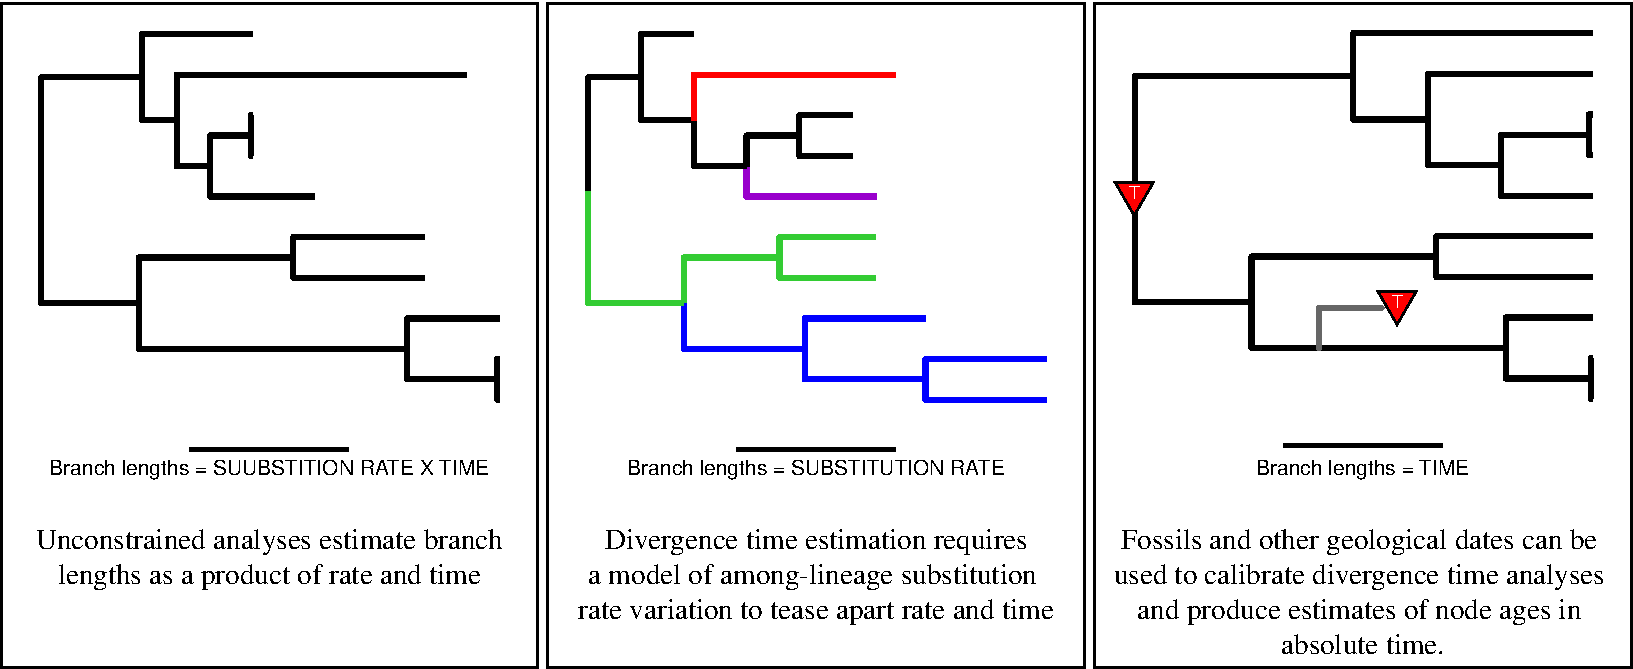
\includegraphics[scale=0.5]{figures/time_rate_cartoon.pdf}}
\caption{\small Estimating branch lengths in units of time requires a model of lineage-specific rate variation, a model for describing the distribution of speciation events over time, and external information to calibrate the tree.}
\label{fig:estBL}
\end{figure}

Ultimately, the goal of Bayesian divergence time estimation is to estimate the joint posterior probability, $\mathbb{P}({\cal R},{\cal T} | {\cal S}, {\cal C})$, of the branch rates (${\cal R}$) and times (${\cal T}$) given a set of sequences (${\cal S}$) and calibration information (${\cal C}$):
$$\mathbb{P}({\cal R},{\cal T} \mid {\cal S}, {\cal C})=\frac{\mathbb{P}({\cal S} \mid {\cal R},{\cal T})\ \mathbb{P}({\cal R})\ \mathbb{P}({\cal T}\mid {\cal C})}{\mathbb{P}({\cal S}\mid {\cal C})},$$
where $\mathbb{P}({\cal S}|{\cal R},{\cal T})$ is the likelihood, $\mathbb{P}({\cal R})$ is the prior probability of the rates, $\mathbb{P}({\cal T} | {\cal C})$ is the prior probability of the times, and $\mathbb{P}({\cal S} | {\cal C})$ is the marginal probability of the data. We use numerical methods---Markov chain Monte Carlo (MCMC)---to eliminate the difficult task of calculating the marginal probability of the data. 
Thus, our primary focus, aside from the tree topology, is devising probability distributions for the prior on the rates, $\mathbb{P}({\cal R})$, and the prior on the times, $\mathbb{P}({\cal T} | {\cal C})$.


\bigskip
\subsection{Modeling lineage-specific substitution rates} 

Many factors can influence the rate of substitution in a population such as mutation rate, population size, generation time, and selection. As a result, many models have been proposed that describe how substitution rate may vary across the Tree of Life. 

The simplest model, the molecular clock, assumes that the rate of substitution remains constant over time \citep{zuckerkandl62}. However, many studies have shown that molecular data (in general) violate the assumption of a molecular clock and that there exists considerable variation in the rates of substitution among lineages.  

Several models have been developed and implemented for inferring divergence times without assuming a strict molecular clock and are commonly applied to empirical data sets. Many of these models have been applied as priors using Bayesian inference methods. The implementation of dating methods in a Bayesian framework provides a flexible way to model rate variation and obtain reliable estimates of speciation times, provided the assumptions of the models are adequate. When coupled with numerical methods, such as MCMC, for approximating the posterior probability distribution of parameters, Bayesian methods are extremely powerful for estimating the parameters of a statistical model and are widely used in phylogenetics.

\textit{Some models of lineage-specific rate variation:}
\begin{itemize}
\item Global molecular clock: a constant rate of substitution over time \citep{zuckerkandl62} 
\item Local molecular clocks \citep{kishino90,rambaut98,yang03, drummond10}  
\begin{itemize}
\item Closely related lineages share the same rate and rates are clustered by sub-clades 
\end{itemize}
\item Compound Poisson process \citep{huelsenbeck00a} 
\begin{itemize}
\item Rate changes occur along lineages according to a point process and at rate-change events, the new rate is a product of the old rate and a $\Gamma$-distributed multiplier. 
\end{itemize}
\item Autocorrelated rates: substitution rates evolve gradually over the tree 
\begin{itemize}
\item Log-normally distributed rates: the rate at a node is drawn from a log-normal distribution with a mean equal to the parent rate \citep{thorne98, kishino01, thorne02}  
\item Cox-Ingersoll-Ross Process: the rate of the daughter branch is determined by a non-central $\chi^2$ distribution. This process includes a parameter that determines the intensity of the force that drives the process to its stationary distribution \citep{lepage06}.
\end{itemize}
\item Uncorrelated rates 
\begin{itemize}
\item The rate associated with each branch is drawn from a single underlying parametric distribution such as an exponential or log-normal \citep{drummond06,rannala07,lepage07}. 
\end{itemize}
\item Mixture model on branch rates 
\begin{itemize}
\item Branches are assigned to distinct rate categories according to a Dirichlet process \citep{heath11}. 
\end{itemize}
\end{itemize}

The variety of models for relaxing the molecular clock assumption presents a challenge for investigators interested in estimating divergence times. Some models assume that rates are heritable and autocorrelated over the tree, others model rate change as a step-wise process, and others assume that the rates on each branch are independently drawn from a single distribution. Furthermore, studies comparing the accuracy (using simulation) or precision of different models have produced conflicting results, some favoring uncorrelated models \citep{drummond06} and others preferring autocorrelated models \citep{lepage07}. Because of this, it is important for researchers performing these analyses to consider and test different relaxed clock models \citep{lepage07,ronquist11,li12,baele13}. It is also critical to take into account the scale of the question when estimating divergence times. For example, it might not be reasonable to assume that rates are autocorrelated if the data set includes very distantly related taxa and low taxon sampling. In such cases, it is unlikely that any signal of autocorrelation is detectible. 

\bigskip
\subsection{Priors on node times}\label{nodepriorsSec} 

There are many component parts that make up a Bayesian analysis of divergence time. One that is often overlooked is the prior on node times, often called a \textit{tree prior}. This model describes how speciation events are distributed over time. When this model is combined with a model for branch rate, Bayesian inference allows you to estimate \textit{relative} divergence times. Furthermore, because the rate and time are confounded in the branch-length parameter, the prior describing the branching times can have a strong effect on divergence time estimation.

We can separate the priors on node ages into different categories:\\
\begin{itemize}
\item \textbf{Phenomenological}---models that make no explicit assumptions about the biological processes that generated the tree. These priors are conditional on the age of the root. 
\begin{itemize}
\item Uniform distribution: This simple model assumes that internal nodes are uniformly distributed between the root and tip nodes \citep{lepage07,ronquist11}.  
\item Dirichlet distribution: A flat Dirichlet distribution describes the placement of internal nodes on every path between the root and tips \citep{kishino01,thorne02}.  
\end{itemize}
\item \textbf{Mechanistic}--models that describe the biological processes responsible for generating the pattern of lineage divergences. 
\begin{itemize}
\item Population-level processes---models describing demographic processes (suitable for describing differences among individuals in the same species/population)  
\begin{itemize}
\item Coalescent---These demographic models describe the time, in generations, between coalescent events and allow for the estimation of population-level parameters \citep{kingman82a,kingman82b,kingman82c,griffiths1994}. 
\end{itemize}
\item Species-level processes---stochastic branching models that describe lineage diversification (suitable for describing the timing of divergences between samples from different species)  
\begin{itemize}
\item Yule (pure-birth) process: The simplest branching model assumes that, at any given point in time, every living lineage can speciate at the same rate, $\lambda$. Because the speciation rate is constant through time, there is an exponential waiting time between speciation events \citet{yule24,aldous01}. The Yule model does not allow for extinction.
\item Birth-death process: An extension of the Yule process, the birth-death model assumes that at any point in time every lineage can undergo speciation at rate $\lambda$ or go extinct at rate $\mu$ \citep{kendall48,thompson75,nee94,rannala96,yang97b,popovic04,Aldous2005,gernhard08}. Thus, the Yule process is a special case of the birth-death process where $\mu=0$. 
\end{itemize}
\end{itemize}
\end{itemize}


%
In BEAST, the available tree priors for divergence time estimation using inter-species sequences are variants of the birth-death prior. 
Extensions of the birth-death model include the calibrated Yule \citep{heled12}, the birth-death model with incomplete species sampling \citep{rannala96,yang97b,stadler09}, and serially-sampled birth-death processes \citep{stadler10}. 
Other programs also offer speciation priors as well as some alternative priors such as a uniform prior (\textit{PhyloBayes}, \textit{MrBayes v3.2}, \textit{DPPDiv}), a Dirichlet prior (\textit{multidivtime}), and a birth-death prior with species sampling (\textit{MCMCTree}). 

Tree priors based on the coalescent which are intended for population-level analyses virus data are also available in BEAST.  The effect of different node-time priors on estimates of divergence times is not well understood and appears to be dataset-dependent \citep{lepage07}. 
Accordingly, it is important to account for the characteristics of your data when choosing a tree prior. 
If you know that your sequences are from extant species, each from different genera, then it is unlikely that a coalescent model adequately reflects the processes that generated those sequences. And since you do not have any samples from lineages in the past, then you should not use the serial-sampled birth-death model. Furthermore, if you have prior knowledge that extinction has occurred, then a pure-birth (Yule) prior is not appropriate. 


\bigskip
\subsection{Calibration to absolute time}\label{calibrationSection} 

Without external information to calibrate the tree, divergence time estimation methods can only reliably provide estimates of relative divergence times and not absolute node ages. 
In the absence of adequate calibration data, relative divergence times are suitable for analyses of rates of continuous trait evolution or understanding relative rates of diversification.
However, for some problems, such as those that seek to uncover correlation between biogeographical events and lineage diversification, an absolute time scale is required.
Calibration information can come from a variety of sources including ``known'' substitution rates (often secondary calibrations estimated from a previous study), dated tip sequences from serially sampled data (typically time-stamped virus data), or geological date estimates (fossils or biogeographical data). 

Age estimates from fossil organisms are the most common form of divergence time calibration information. These data are used as age constraints on their putative ancestral nodes. There are numerous difficulties with incorporating node age estimates from fossil data including disparity in fossilization and sampling, uncertainty in dating, and correct phylogenetic placement of the fossil. Thus, it is critical that careful attention is paid to the paleontological data included in phylogenetic divergence time analyses. 
With an accurately dated and identified fossil in hand, further consideration is required to determine how to apply the node-age constraint. If the fossil is truly a descendant of the node it calibrates, then it provides a reliable minimum age bound on the ancestral node time. However, maximum bounds are far more difficult to come by. Bayesian methods provide a way to account for uncertainty in fossil calibrations. Prior distributions reflecting our knowledge (or lack thereof) of the amount of elapsed time from the ancestral node to its calibrating fossil are easily incorporated into these methods. 

A nice review paper by \citet{ho09} outlines a number of different parametric distributions appropriate for use as priors on calibrated nodes. 
%In this exercise we will use the uniform, normal, log-normal, and exponential distributions (Figure \ref{fig:calPriors}).  
\begin{figure}[h!]
\centering
\fbox{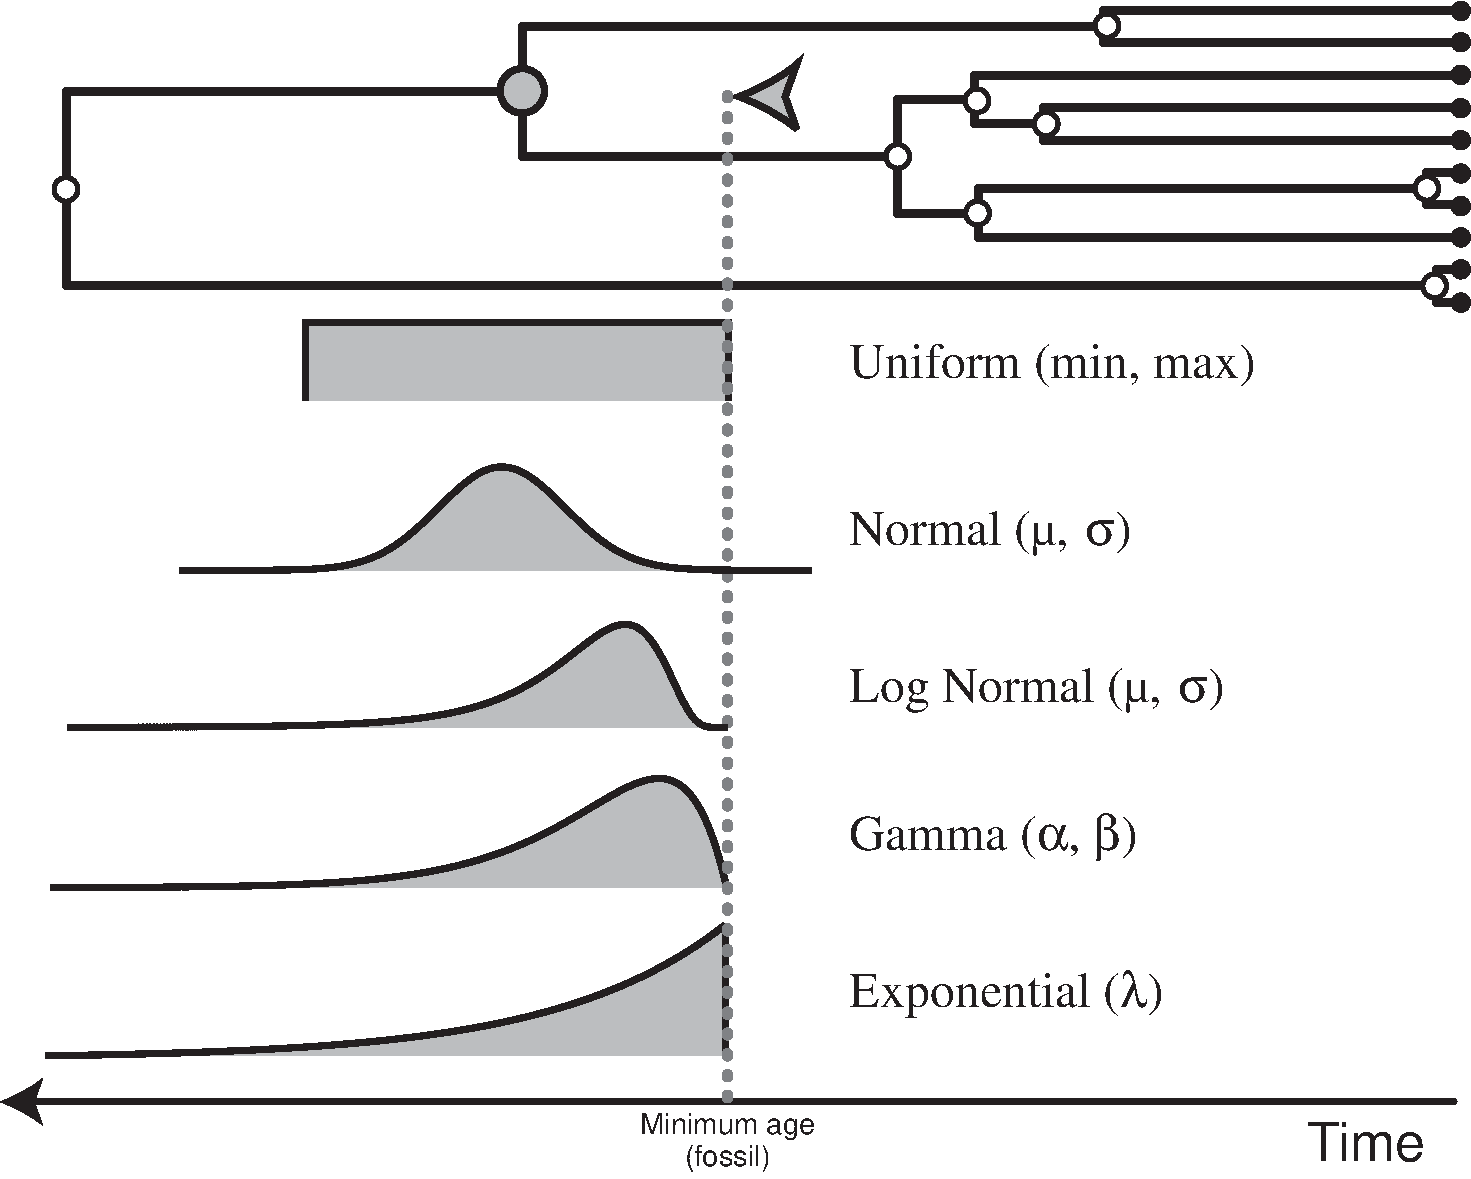
\includegraphics[width=3in]{figures/cal_priors.pdf}}
\caption{\small Five different parametric distributions that can be applied as priors on the age of a calibrated node. \citep[figure adapted from][]{heath12}}
\label{fig:calPriors}
\end{figure}

\textit{Uniform distribution} -- Typically, you must have both maximum and minimum age bounds when applying a uniform calibration prior (though some methods are available for applying uniform constraints with soft bounds). The minimum bound is provided by the fossil member of the clade. The maximum bound may come from a bracketing method or other external source. This distribution places equal probability across all ages spanning the interval between the lower and upper bounds. 

\textit{Normal distribution} -- The normal distribution is not always appropriate for calibrating a node using fossil information (though some methods allow for assigning a truncated normal prior density). When applying a biogeographical date (e.g. the Isthmus of Panama) or a secondary calibration (a node age estimate from a previous study), the normal distribution can be a useful calibration prior. This distribution is always symmetrical and places the greatest prior weight on the mean ($\mu$). Its scale is determined by the standard deviation parameter ($\sigma$).

Probability distributions restricted to the interval $[0,\infty)$, such as the log-normal, exponential, and gamma are appropriate for use as zero-offset calibration priors. When applying these priors on node age, the fossil age is the origin of the prior distribution. Thus, it is useful to consider the fact that the prior is modeling the amount of time that has elapsed since the divergence event (ancestral node) until the time of the descendant fossil (Figure \ref{fig:lnExpPriors}). 
\begin{figure}[h!]
\centering
\fbox{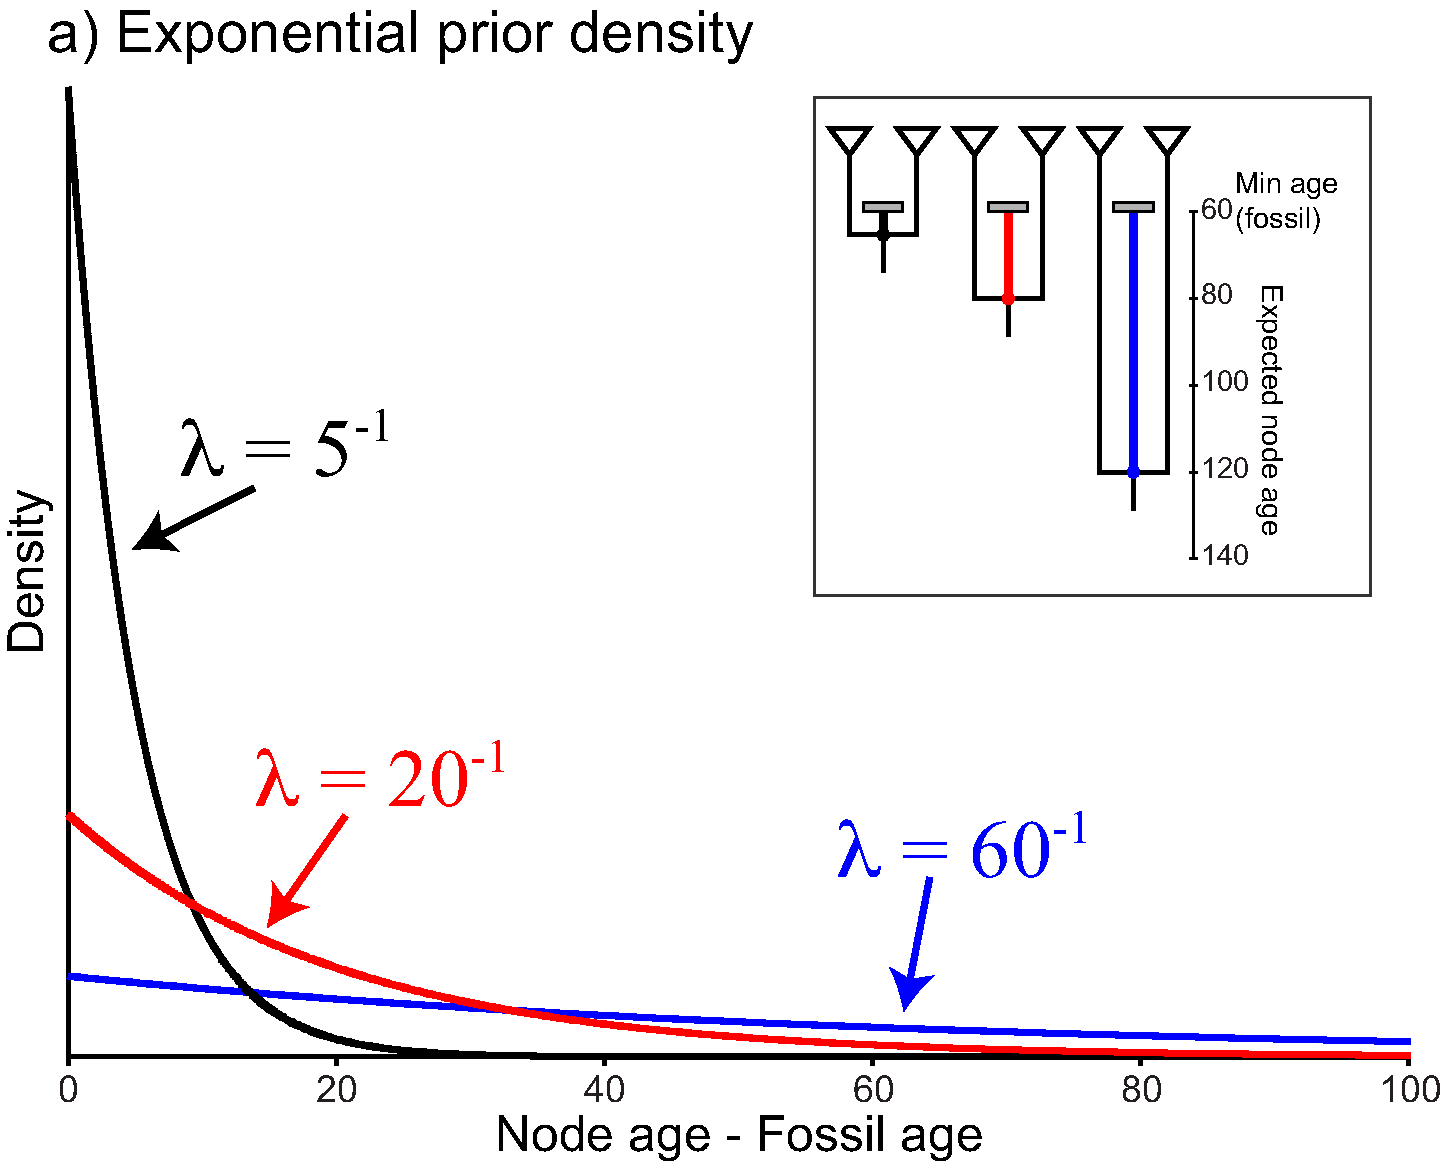
\includegraphics[scale=0.31]{figures/exponential_dist_example2.pdf}}\hspace{2mm}
\fbox{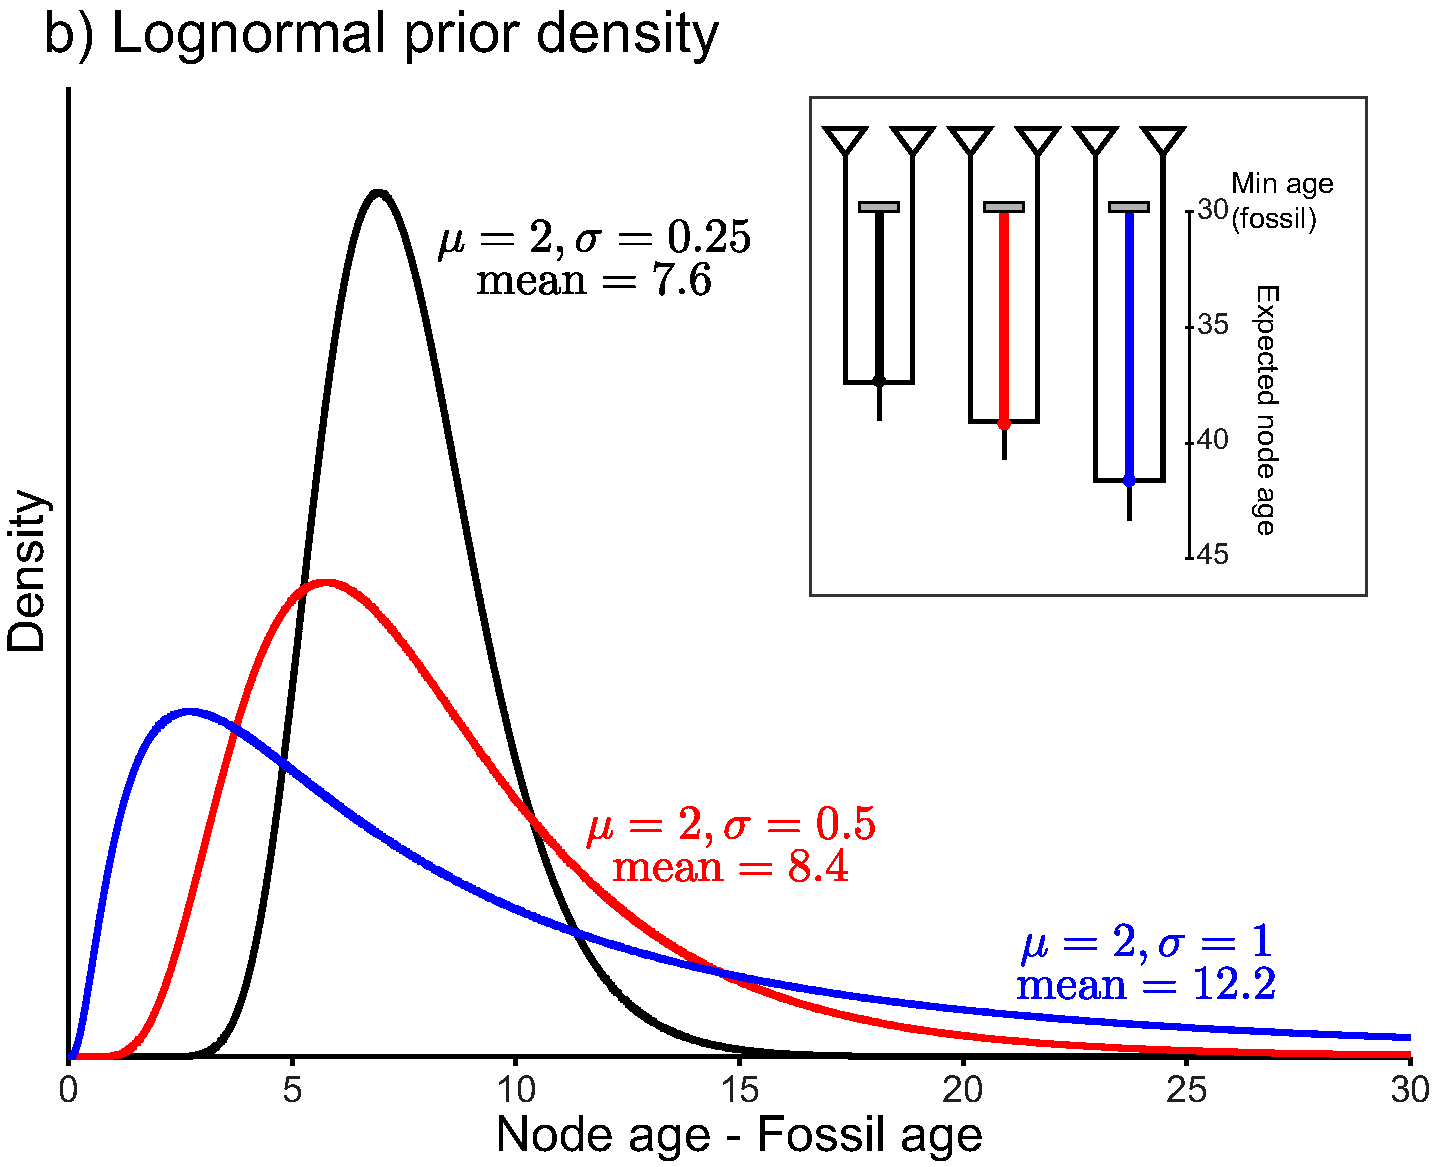
\includegraphics[scale=0.31]{figures/lognormal_example.pdf} } %\hspace{2mm}
\caption{\small Two common prior densities for calibrating node ages. a) The exponential distribution with three different values for the rate parameter, $\lambda$. As the value of the $\lambda$ rate parameter is decreased, the prior becomes less informative (the blue line is the least informative prior, $\lambda=60^{-1}$). The inset shows an example of the three different priors and their expected values placed on the same node with a minimum age bound of 60. b) The lognormal distribution with 3 different values for the shape parameter, $\sigma$. For this distribution, even though $\mu$ is equal to 2.0 for all three, expected value (mean) is dependent on the value of $\sigma$. The inset shows an example of the three different priors and their expected values placed on the same node with a minimum age bound of 30. }
\label{fig:lnExpPriors}
\end{figure}

\textit{Gamma distribution} -- The gamma distribution is commonly used as a prior on scalar variables in Bayesian inference. It relies on 2 parameters: the scale parameter ($\alpha$) and a rate parameter ($\lambda$). More specifically, the gamma distribution is the sum of $\alpha$ independently and identical exponentially distributed random variables with rate $\lambda$. As $\alpha$ becomes very large ($\alpha > 10$), this distribution approaches the normal distribution. 

\textit{Exponential distribution} -- The exponential distribution is a special case of the gamma distribution and is characterized by a single rate parameter ($\lambda$) and is useful for calibration if the fossil age is very close to the age of its ancestral node. The expected (mean) age difference under this distribution is equal to $\lambda^{-1}$ and the median is equal to $\lambda^{-1} * ln(2)$. Under the exponential distribution, the greatest prior weight is placed on node ages very close to the age of the fossil with diminishing probability to $\infty$. As $\lambda$ is increased, this prior density becomes strongly informative, whereas very low values of $\lambda$ result in a fairly non-informative prior (Figure \ref{fig:lnExpPriors}a).

\textit{Log-normal distribution} -- An offset, log-normal prior on the calibrated node age places the highest probability on ages somewhat older than the fossil, with non-zero probability to $\infty$. If a variable is log-normally distributed with parameters $\mu$ and $\sigma$, then the natural log of that variable is normally distributed with a mean of $\mu$ and standard deviation of $\sigma$. The median of the lognormal distribution is equal to $e^{\mu}$ and the mean is equal to $e^{\mu + \frac{\sigma^2}{2}}$ (Figure \ref{fig:lnExpPriors}b). 

\bigskip
\subsection{Integrating Fossil Occurrence Times in the Speciation Model} 

Calibrating Bayesian divergence-time estimates using parametric densities (as described in the previous section: Sec.~\ref{calibrationSection}) is ultimately a difficult and unsatisfactory approach, particularly if the calibration information comes from fossil occurrence times. 
The calibration densities are typically applied in a multiplicative manner such that the prior probability of a calibrated node age is the product o the probability coming from the tree-wide speciation model and the probability under the calibration density \citep{heled12,warnock12,warnock2015}. 
This approach leads to an incoherence and induces a prior that is inconsistent with the described calibration density. 
This statistical incoherence has been corrected by conditional tree prior models \citep{yang06,heled12,heleddrummond2013}. 
These conditional approaches are an important contribution to the field, particularly when non-fossil data are used to calibrate an analysis.
However, when using fossil information, it is more appropriate to account for the fact that the fossils are part of the same diversification process (\textit{i.e.}, birth-death model) that generated the extant species. 
%Thus, new models that jointly estimate the tree of extant and fossil species and divergence times \citep{lee09,pyron11,ronquist11} and  integrate the fossil observations into the diversification model \citep{stadler10,heath2013fossilized,gavryushkina2014} are an important direction for estimating speciation times on an absolute timescale.

\bigskip
\subsubsection{The Fossilized Birth-Death Process}\label{FBDSection}

The exercise outlined in this tutorial demonstrates how to calibrate species divergence using the \textit{fossilized birth-death} (FBD) model described in \citet{stadler10} and \citet{heath2013fossilized}. 
This model simply treats the fossil observations as part of the prior on node times, such as the birth-death models outlined in Section \ref{nodepriorsSec} of this document. 
The fossilized birth-death process provides a model for the distribution of speciation times, tree topology, and distribution of lineage samples before the present (i.e., non-contemporaneous samples like fossils or viruses). 
Importantly, this model can be used \textit{with or without} character data for the historical samples. 
Thus, it provides a reasonable prior distribution for analyses combining morphological or DNA data for both extant and fossil taxa---i.e, the so-called `total-evidence' approaches described by \citet{ronquist11} \citep[also see][]{pyron11}. 
When matrices of discrete morphological characters for both living and fossil species are unavailable, the fossilized birth-death model imposes a time structure on the tree by \textit{marginalizing} over all possible attachment points for the fossils on the extant tree \citep{heath2013fossilized}, therefore, some prior knowledge of phylogenetic relationships is important, much like for calibration-density approaches. 

The FBD model describes the probability of the tree and fossils conditional on the birth-death parameters: $f[\mathcal{T} \mid \lambda, \mu, \rho, \psi, x_c]$, where $\mathcal{T}$ denotes the tree topology, divergence times, fossil occurrence times, and the times at which the fossils attach to the tree.
The parameters of the model are:
\begin{center}
\begin{tabular}{l c r}
\hline
$\lambda$ & & speciation rate\\
$\mu$ & & extinction rate\\
$\rho$ & & probability of sampling extant species\\
$\psi$ & & fossil recovery rate\\
$x_c$ & & the starting time of the process, either $x_0$ or $x_1$\\
\hline
\end{tabular}
\end{center}
Figure \ref{fig:FBD}A shows the probabilistic graphical model of the FBD process.
Additionally, an example FBD tree is shown in Figure \ref{fig:FBD}B, where the diversification process originates at time $x_0$, giving rise to $n=20$ species in the present.
All of the lineages represented in Figure \ref{fig:FBD}B (both solid and dotted lines) show the \textit{complete tree}. 
This is the tree of all extant \textit{and} extinct lineages generated by the process.
The complete tree is distinct from the \textit{reconstructed tree} which is the tree representing only the sampled \textit{extant} lineages.
Fossil observations (red circles in Figure \ref{fig:FBD}B) are recovered over the process along the lineages of the complete tree. 
If a lineage does not have any descendants sampled in the present, it is lost and cannot be observed, these are the dotted lines in Figure \ref{fig:FBD}B. 
The probability must be conditioned on the starting time of the process $x_c$. This can be one of two different nodes in the tree, either the origin time $x_0$ or the root age $x_1$ (Figure \ref{fig:FBD}B).
The origin ($x_0$) of a birth death process is the starting time of the \textit{stem} lineage, thus this conditions on a single lineage giving rise to the tree.
Alternatively, a birth-death process can be conditioned on the age of the root ($x_1$), which is the time of the most-recent-common ancestor (MRCA) of the sampled lineages.
Here, the model assumes that the branching process starts with two lineages, each of which has the same starting time. 

An important characteristic of the FBD model is that it accounts for the probability of sampled ancestor-descendant pairs \citep{foote1996}. 
Given that fossils are sampled from lineages in the diversification process, the probability of sampling fossils that are ancestors to taxa sampled at a later date is correlated with the turnover rate ($r=\mu/\lambda$) and the fossil recovery rate ($\psi$).
This feature is important, particularly for datasets with many sampled fossils. 
In the example (Figure \ref{fig:FBD}B), several of the fossils have sampled descendants. These fossils have solid black lines leading to the present. 


\begin{figure}[h!]
\centering
\fbox{A)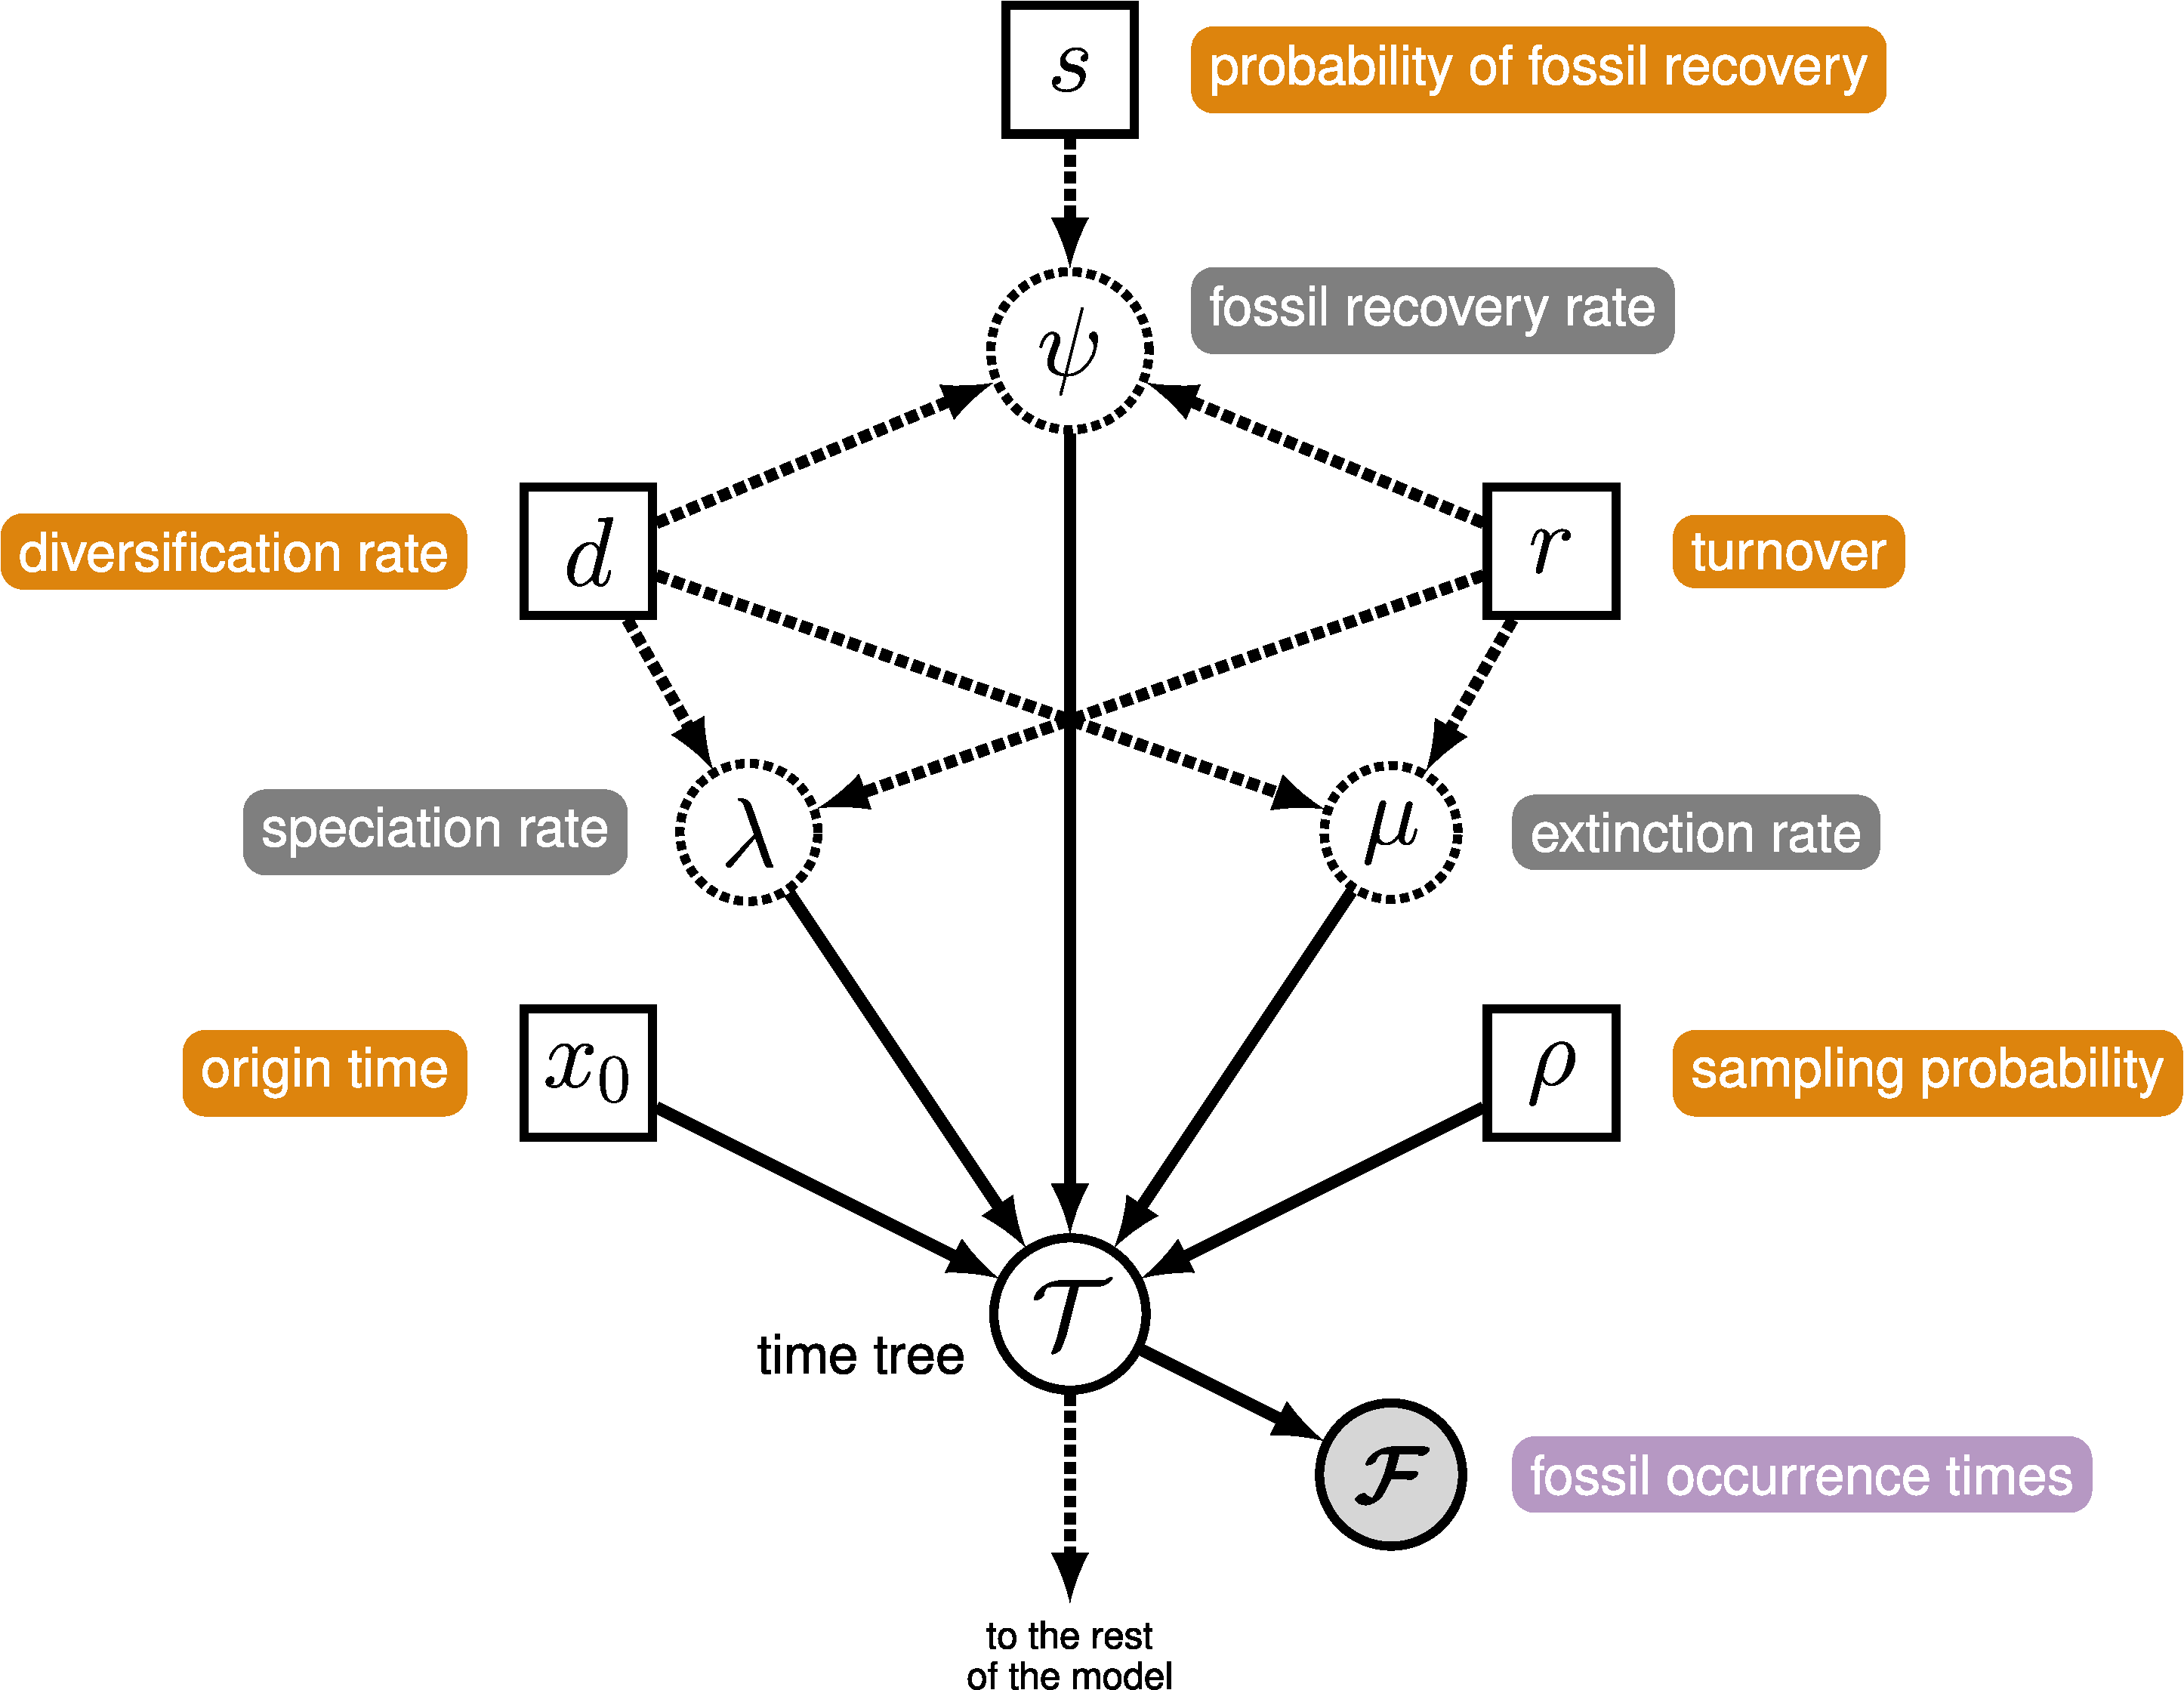
\includegraphics[height=2.65in]{figures/FBD_gm.pdf}}
\fbox{B)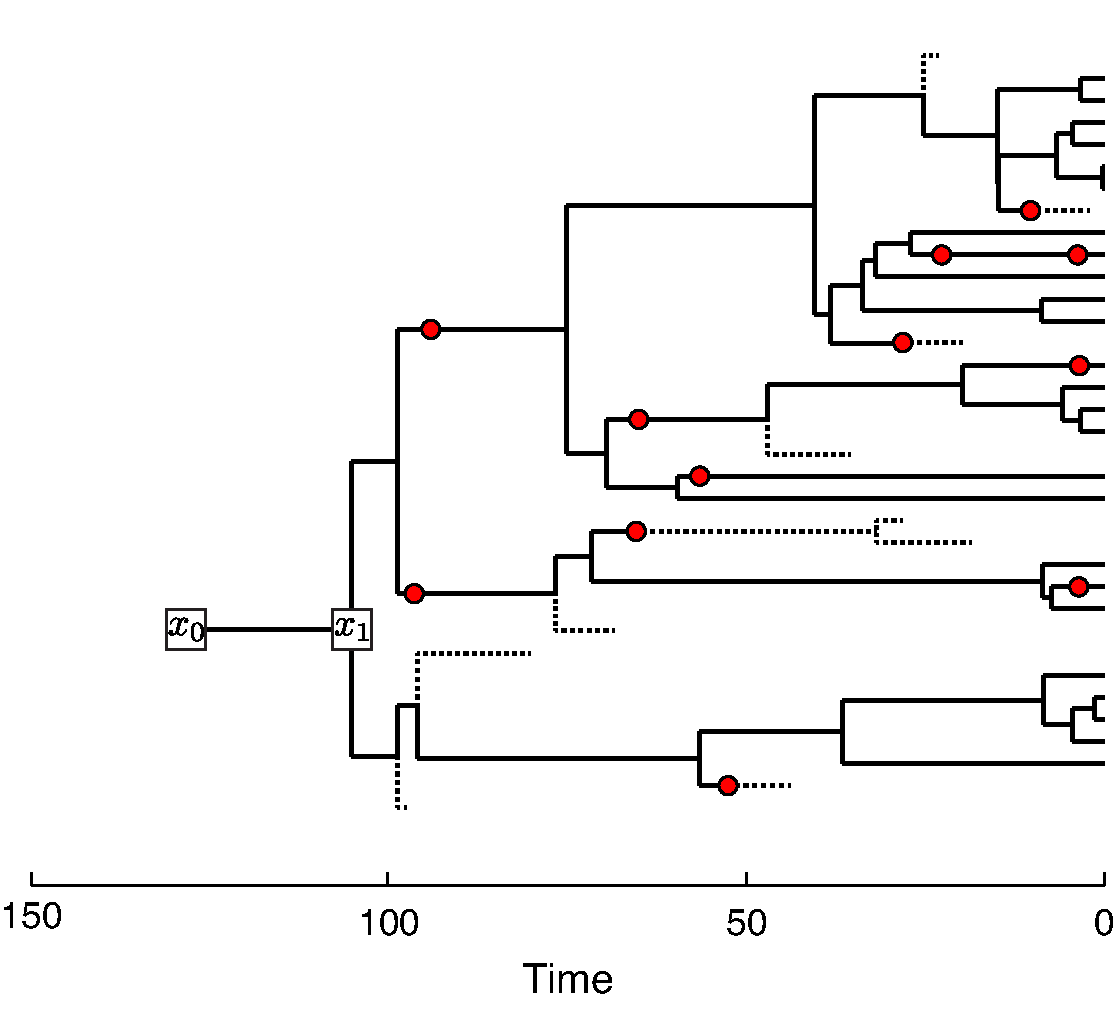
\includegraphics[height=2.65in]{figures/tree_plot_with_fossils.pdf}}
\caption{\small The \textit{fossilized birth-death process}. (A) The probabilistic graphical model of the FBD process for divergence-time estimation. All of the relevant parameters are labeled, with square-shaped nodes representing constant parameters, circles with solid borders indicate stochastic variables, deterministic nodes are shown in circles with dotted borders, and shaded nodes indicate observed variables. This model connects to the rest of the phylogenetic continuous-time Markov model through the time-tree variable. (B) A FBD tree generated by single realization of the process; simulated with the parameters: $\lambda=0.02,\mu=0.01,\psi=0.01,\rho=1$. The red circles represent recovered fossil occurrence times. Sampled lineages are shown with solid black lines and unobserved lineages with dotted lines.}
\label{fig:FBD}
\end{figure}


Recently, \citet{gavryushkina2014} extended the fossilized birth-death model to allow more flexibility in the assignment of fossils to clades and conditioning parameters and implemented this version in the BEAST2 package called \textbf{SA} (``Sampled Ancestors'', by Alexandra Gavryushkina). 
Notably, this implementation also allows you to use the FBD model as a tree prior for datasets combining molecular data from extant taxa with morphological data for both fossil and extant species. 
In this implementation of the FBD model, instead of the parameters $\lambda$, $\mu$, and $\psi$, the following parameters are used in MCMC optimization:
\begin{center}
\begin{tabular}{rcl}
\hline
$d=\lambda-\mu$ & \hspace{6mm} & Net diversification rate\\
$r=\mu / \lambda$ & & Turnover\\
$s=\psi / (\mu+\psi)$ & & Probability of fossil observation %recovery 
prior to species extinction\\
\hline
\end{tabular} 
\end{center}
The parameters $\lambda$, $\mu$, and $\psi$ needed for the FBD probability are recovered via: 
$$\lambda=\frac{d}{1-r}, \quad \mu=\frac{rd}{1-r}, \quad \psi = \frac{s}{1-s} \frac{rd}{1-r}.$$
Conveniently, under the $d,r,s,\rho$ parameterization, three parameters $r,s,\rho \in [0,1]$, with only $d$ 
on the interval $(0,\infty)$, thus, this allows for easier prior distribution construction under this model \citep{heath2013fossilized}.
Furthermore, it is important to carefully consider the relevant parameters of the birth-death process and the choice of the $d,r,s$ parameterization allows for estimation of the diversification rate and turnover rate. Typically, macroevolutionary studies are interested in these parameters.

The fossilized birth-death process provides a way to integrate fossil occurrence times into the tree prior and is currently the most appropriate way to calibrate divergence time estimates when the calibration dates represent fossil occurrence times. 
However, this approach is not suitable for dating trees using biogeographical information or secondary calibration dates. 
In these cases, it is better to use conditioned birth-death processes \citep{yang06,heled12,heleddrummond2013}.
Furthermore, advances in methods for modeling historical biogeography \citep{landis2013} also present some exciting potential for accommodating this information in methods for dating species divergences. 



\clearpage
\newpage
\section{Programs used in this Exercise}\label{programsSec}

\descriptionhead{BEAST -- Bayesian Evolutionary Analysis Sampling Trees}

BEAST is a free software package for Bayesian evolutionary analysis of molecular sequences using MCMC and strictly oriented toward inference using rooted, time-measured phylogenetic trees \citep{drummond06,drummond07,Bouckaert2014}. The development and maintenance of BEAST is a large, collaborative effort and the program includes a wide array of different types of analyses:

\begin{itemize}
\item Phylogenetic tree inference under different models for substitution rate variation 
\begin{itemize}
\item Constant rate molecular clock \citep{zuckerkandl62} 
\item Uncorrelated relaxed clocks \citep{drummond06} 
\item Random local molecular clocks \citep{drummond10} 
\end{itemize}
\item Estimates of species divergence dates and fossil calibration under a wide range of branch-time models and calibration methods 
\item Analysis of non-contemporaneous sequences
\item Heterogenous substitution models across data partitions 
\item Population genetic analyses
\begin{itemize}
\item Estimation of demographic parameters (population sizes, growth/decline, migration) 
\item Bayesian skyline plots
\item Phylogeography \citep{lemey09}
\end{itemize}
\item Gene-tree/species-tree inference \citep[$*$BEAST;][]{heled10} 
\item and more...
\end{itemize}

BEAST is written in java and its appearance and functionality are consistent across platforms. Inference using MCMC is done using the BEAST program, however, there are several utility applications that assist in the preparation of input files and summarize output (BEAUti, LogCombiner, and TreeAnnotator are all part of the BEAST software bundle). 

There are currently two available versions of the BEAST package:
\begin{description}[labelindent=0.5cm]
\item[BEAST v1.8] \href{http://beast.bio.ed.ac.uk}{http://beast.bio.ed.ac.uk} (BEAST 1)
\item[BEAST v2$*$] \href{http://www.beast2.org/}{http://www.beast2.org} (BEAST 2).
\end{description} 

BEAST 2 is a complete re-write of BEAST 1, with different design choices \citep{Bouckaert2014}.
The BEAST 2 package allows for implementation and distribution of new models and methods through \textit{add-ons} (also called ``plugins'').
Add-ons include \href{http://www.beast2.org/wiki/index.php/SNAPP}{SNAPP} (phylogenetic analysis using SNP and AFLP data) and \href{https://code.google.com/p/bdssm-beast2/}{BDSSM} (a birth-death skyline model for serially-sampled data), as well as several others that are available or in development.
It is important to note, however, that the set of analyses and models available in the BEAST 2 package do not completely overlap with the set of analyses with BEAST 1 (though this should not be the case in the near future).
I strongly encourage you to learn more about BEAST and the BEAST v2 software by reading the book provided online by the developers: \href{http://www.beast2.org/book.html}{\textit{Bayesian Evolutionary Analysis with BEAST 2}}  \citep{BEAST2book2014}.

\descriptionhead{BEAUti -- Bayesian Evolutionary Analysis Utility}

BEAUti is a utility program with a graphical user interface for creating BEAST and *BEAST input files which must be written in the eXtensible Markup Language (XML). This application provides a clear way to specify priors, partition data, calibrate internal nodes, etc.

\dhead{LogCombiner} 
When multiple (identical) analyses are run using BEAST (or MrBayes), LogCombiner can be used to combine the parameter log files or tree files into a single file that can then be summarized using Tracer (log files) or TreeAnnotator (tree files). However, it is important to ensure that all analyses reached convergence and sampled the same stationary distribution before combining the parameter files.

\dhead{TreeAnnotator} 
TreeAnnotator is used to summarize the posterior sample of trees to produce a maximum clade credibility tree and summarize the posterior estimates of other parameters that can be easily visualized on the tree (e.g. node height). This program is also useful for comparing a specific tree topology and branching times to the set of trees sampled in the MCMC analysis. 

\dhead{Tracer} 
Tracer is used for assessing and summarizing the posterior estimates of the various parameters sampled by the Markov Chain. This program can be used for visual inspection and assessment of convergence and it also calculates 95\% credible intervals (which approximate the 95\% highest posterior density intervals) and effective sample sizes (ESS) of parameters (\href{http://beast.community/tracer}{http://beast.community/tracer}).

\dhead{FigTree} 
FigTree is an excellent program for viewing trees and producing publication-quality figures. It can interpret the node-annotations created on the summary trees by TreeAnnotator, allowing the user to display node-based statistics (e.g. posterior probabilities) in a visually appealing way (\href{http://tree.bio.ed.ac.uk/software/figtree}{\small http://tree.bio.ed.ac.uk/software/figtree}). 


\bigskip
\section{The eXtensible Markup Language}

The eXtensible Markup Language (XML) is a general-purpose markup language, which allows for the combination of text and additional information. In BEAST, the use of the XML makes analysis specification very flexible and readable by both the program and people. The XML file specifies sequences, node calibrations, models, priors, output file names, etc. BEAUti is a useful tool for creating an XML file for many BEAST analyses. However, typically, dataset-specific issues can arise and some understanding of the BEAST-specific XML format is essential for troubleshooting. Additionally, there are a number of interesting models and analyses available in BEAST that cannot be specified using the BEAUti utility program. Refer to the BEAST web page (\href{http://beast.bio.ed.ac.uk/XML_format}{http://beast.bio.ed.ac.uk/XML\_format}) for detailed information about the BEAST XML format. Box 1 shows an example of BEAST XML syntax for specifying a birth-death prior on node times. 

%{\tt \scriptsize{\begin{framed} \begin{tabbing}
%\textless !-- A prior on the distribution node heights defined given \ \ \ \ \ \ \ \ \ \ \ \ \ \ \ \ \ \ \ \ \ \ \ \ \ \ \ \ \ \ \ \ --\textgreater\\
%\textless !-- a Birth-Death speciation process (Gernhard 2008). \ \ \ \ \ \ \ \ \ \ \ \ \ \ \ \ \ \ \ \ \ \ \ \ \ \ \ \ \ \ \ \ \ \ \ \ --\textgreater\\
%\textless bir\=thDeathModel id="birthDeath" units="substitutions"\textgreater\\
%\> \textless bir\=thMinusDeathRate\textgreater\\
%\> \> \textless parameter id="birthDeath.meanGrowthRate" value="1.0" lower="0.0" upper="Infinity"/\textgreater\\
%\> \textless /birthMinusDeathRate\textgreater\\
%\> \textless relativeDeathRate\textgreater\\
%\> \> \textless parameter id="birthDeath.relativeDeathRate" value="0.5" lower="0.0" upper="Infinity"/\textgreater\\
%\> \textless /relativeDeathRate\textgreater\\
%\textless /birthDeathModel\textgreater
%\end{tabbing}\end{framed}}}

\begin{center}
{\tt \scriptsize{\begin{minipage}{6.5in}
\begin{lstlisting}[language=XML]
<!- An exponential prior distribution on the gamma shape parameter of the irbp gene   ->
<prior id="GammaShapePrior.s:irbp" name="distribution" x="@gammaShape.s:irbp">
    <Exponential id="Exponential.01" name="distr">
        <parameter id="RealParameter.01" lower="0.0" name="mean" upper="0.0">1.0</parameter>
    </Exponential>
</prior>
\end{lstlisting}
\end{minipage}}}\\\vspace{4mm}
Box 1: BEAST 2 XML specification of an exponential prior density on the shape of a gamma distribution.\\
\end{center}

\newpage
\section{Practical: Divergence Time Estimation}

%\bigskip
%\subsection{Introduction}

This tutorial will walk you through an analysis of the divergence times of the bears.
The occurrence times of 14 fossil species are integrated into the tree prior to impose a time structure on the tree and calibrate the analysis to absolute time.
Additionally, an uncorrelated, lognormal relaxed clock model is used to describe the branch-specific substitution rates.

Make sure you have already downloaded the software listed in Section \ref{programsSec}.
%% More stuff here.

%\begin{figure}[h!]
%\centering
%\fbox{\includegraphics[width=4in]{figures/FBD_MS_fig4-rev.eps}}
%\caption{\small The divergence times of extant bears and two caniform outgroups estimated under the fossilized birth-death process. Reproduced from Figure 4 of \citet{heath2013fossilized}.}
%\label{packageManage}
%\end{figure}

%\begin{table}[tbh!]
%\centering
%\caption{Fossil species used for calibrating divergence times in the caniform tree.}\label{bearFossilTable}
%\begin{tabular}{@{\extracolsep{\fill}}l  c c c r}
%\hline
%\multicolumn{1}{@{}l}{\textbf{Fossil species}}  & &\multicolumn{1}{c}{\textbf{Age range (My)}}  & &\multicolumn{1}{c}{\textbf{Citation}} \\ 
%\hline
%\textit{Hesperocyon gregarius} & \hspace{2mm} & 37.2--40 & \hspace{2mm} & \cite{wang1994,wang1999}\\
%\textit{Parictis montanus} & & 33.9--37.2 &  & \cite{clark1972,krause2008}\\
%\textit{Kretzoiarctos beatrix} & & 11.2--11.8 &  & \cite{abella2011,abella12}\\
%\hline
%\end{tabular}
%\end{table}

\bigskip
\subsection{The Data}

\begin{framed}
Download data and pre-cooked output files from:
\begin{center}
\href{https://taming-the-beast.github.io/tutorials/FBD-tutorial/}{https://taming-the-beast.github.io/tutorials/FBD-tutorial}
%The data folder of this tutorial
%
%or
%
%\href{http://treethinkers.org/divergence-time-estimation-using-beast/}{http://treethinkers.org/divergence-time-estimation-using-beast} 
\end{center}
\end{framed}

The analysis in this tutorial includes data from several different sources.
We have molecular sequence data for eight extant species, which represent all of the living bear taxa.
The sequence data include interphotoreceptor retinoid-binding protein (irbp) sequences (in the file \cl{bears\_irbp\_fossils.nex})
and 1000 bps of the mitochondrial gene cytochrome b (in the file  \cl{bears\_cytb\_fossils.nex}).
If you open either of these files in your text editor or alignment viewer, you will notice that there are 22 taxa listed in each one, with most of these taxa associated with sequences that are entirely made up of missing data (i.e., \cl{?????}). 
The NEXUS files contain the names of 14 fossil species, that we will include in our analysis as calibration information for the fossilized birth-death process. 
Further, we must provide an occurrence time for each taxon sampled from the fossil record.
For the fossil species, this information is obtained from the literature or fossil databases like the \href{http://fossilworks.org/}{Fossilworks PaleoDB} or the \href{http://fossilcalibrations.org/}{Fossil Calibration Database}, or from your own paleontological expertise. 
The 14 fossil species used in this analysis are listed in Table \ref{bearFossilTable} along with the age range for the specimen and relevant citation.
For this exercise, we will fix the ages to a value within the age range provided in Table \ref{bearFossilTable}. 
In BEAST2, it is possible to use MCMC to sample the occurrence time for a fossil conditional on a prior distribution. 
However, the options to do this are not currently available in BEAUti, and will not be covered by this tutorial.
The age of each taxon is encoded in the taxon name following the last `\cl{\_}' character. 
For example, the fossil panda \textit{Kretzoiarctos beatrix} has an age of approximately 11.7 Mya, thus, the taxon name in the alignment files is: \cl{Kretzoiarctos\_beatrix\_11.7}.
Similarly, since the polar bear, \textit{Ursus maritimus}, represents an extant species, its occurrence time is 0.0 Mya, which makes its taxon name: \cl{Ursus\_maritimus\_0}.
By including the tip ages in the taxon names, we can easily import these values into BEAUti while setting up the XML file. 
This is simply easier than entering them in by hand (which is also possible).

%The data used in this tutorial include two alignment in files \cl{bears\_irbp.nex} contains interphotoreceptor retinoid-binding protein (irbp) sequences for each extant species.

\begin{table}[tbh!]
\centering
\caption{Fossil species used for calibrating divergence times under the FBD model. Modified from Table S.3 in the supplemental appendix of \citet{heath2013fossilized}.}\label{bearFossilTable}
{\small
\begin{tabular}{@{\extracolsep{\fill}}l  c c c r}
\hline
\multicolumn{1}{@{}l}{\textbf{Fossil species}}  & &\multicolumn{1}{c}{\textbf{Age range (My)}}  & &\multicolumn{1}{r}{\textbf{Citation}} \\ 
\hline
\hspace{2mm} \textit{Parictis montanus} & & 33.9--37.2 & & \cite{clark1972,krause2008}\\
\hspace{2mm} \textit{Zaragocyon daamsi} & & 20--22.8  & & \cite{ginsburg1995,abella12}\\
\hspace{2mm} \textit{Ballusia elmensis} & & 13.7--16 & & \cite{ginsburg1998,abella12}\\
\hspace{2mm} \textit{Ursavus primaevus} & & 13.65--15.97 & & \cite{andrews1977,abella12}\\
\hspace{2mm} \textit{Ursavus brevihinus} & & 15.97--16.9  & & \cite{heizmann1980,abella12}\\
\hspace{2mm} \textit{Indarctos vireti} & & 7.75--8.7  & & \cite{montoya2001,abella12}\\
\hspace{2mm} \textit{Indarctos arctoides} & & 8.7--9.7 & & \cite{geraads2005,abella12}\\
\hspace{2mm} \textit{Indarctos punjabiensis} & & 4.9--9.7 & & \cite{baryshnikov2002,abella12}\\
\hspace{2mm} \textit{Ailurarctos lufengensis} & & 5.8--8.2 & & \cite{jin2007,abella12}\\
\hspace{2mm} \textit{Agriarctos spp.} & & 4.9--7.75 && \cite{abella2011,abella12}\\
\hspace{2mm} \textit{Kretzoiarctos beatrix} & & 11.2--11.8 & & \cite{abella2011,abella12}\\
\hspace{2mm} \textit{Arctodus simus} & & 0.012--2.588 & & \cite{churcher1993,krause2008}\\
\hspace{2mm} \textit{Ursus abstrusus} & & 1.8--5.3 & & \cite{bjork1970,krause2008}\\
\hspace{2mm} \textit{Ursus spelaeus} & & 0.027--0.25 & & \cite{loreille2001,krause2008}\\
\hline
\end{tabular}}
\end{table}

The final source of data required for our analysis is some information about the phylogenetic placement of the fossils. 
This prior knowledge can come from previous studies of morphological data and taxonomy.
Ideally, we would know exactly where in the phylogeny each fossil belongs. 
However, this is uncommon for most groups in the fossil record. 
Often, we can place a fossil with reasonable resolution by assigning it to some total group. 
For example, if a fossil specimen has all of the identifying characters of a bear in the subfamily Ursinae, then, we can create a monophyletic group of all known Ursinae species and our fossil.
Here, we would be assigning the fossil to the \textit{total group} Ursinae, meaning that the fossil can be a crown or stem fossil of this group. 
For some fossils, we may have very little data to inform their placement in the tree and perhaps we may only know that it falls somewhere within our group of interest. 
In this case, we can account for our uncertainty in the relationship of the fossil and all other taxa and allow MCMC to sample all possible places where the fossil can attach in the tree. 
For the bear species in our analysis, we have some prior knowledge about their relationships, represented as an unresolved phylogeny in Figure \ref{fig:clades}.
Four out of five of the clades shown in Figure \ref{fig:clades} are defined in the NEXUS file \cl{bears\_cytb\_fossils.nex} as \cl{taxsets} in the \cl{sets} block. 
The one clade that is not included in the data file will be created using the BEAUti options. 

\begin{figure}[h!]
\centering
\fbox{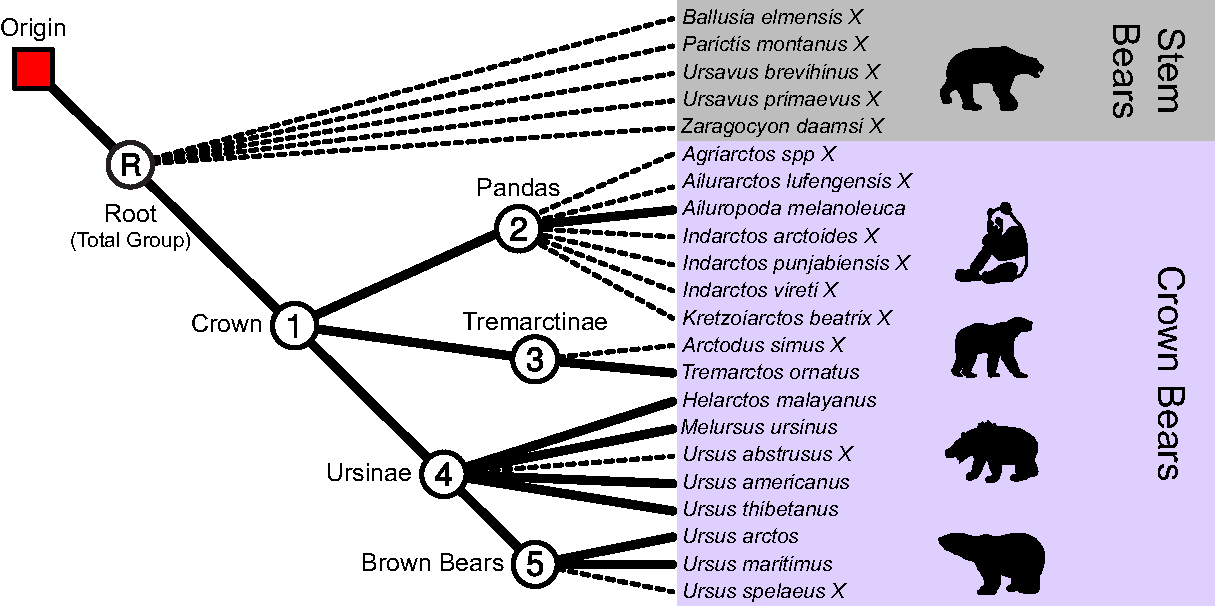
\includegraphics[width=5in]{figures/bears_clades_tree.pdf}}
\caption{\small The phylogenetic relationships of crown and stem bears based on taxonomy and morphological data. The resolution of monophyletic clades is based on well-supported previous analyses. Monophyletic clades are indicated with labeled circles. In addition to the root node (R), there are 5 nodes defining clades containing both fossil and extant species. The origin of the tree is indicated with a red square. The time of this node represents the start of the diversification process that generated these linages. 
The extant lineages are shown with heavy, solid lines and the fossil lineages are dotted lines.}
\label{fig:clades}
\end{figure}


\bigskip
\subsection{Creating the Analysis File with BEAUti}

Creating a properly-formatted BEAST XML file from scratch is not a simple task. However, BEAUti provides a simple way to navigate the various elements specific to the BEAST XML format. 

\begin{framed}
Begin by executing the BEAUti program
\end{framed}
Be sure that this is the version that came from the BEAST 2 download from: \href{http://beast2.org/}{http://beast2.org}. For Mac OSX and Windows, you can do this by double clicking on the application. For Unix systems (including Mac OSX), it is convenient to add the entire \cl{BEAST/bin} directory to your path.


\bigskip
\subsubsection{Install BEAST 2 Plug-Ins}

Next, we have to install the BEAST 2 packages (also called ``plug-ins'' or ``add-ons'') that are needed for this analysis. 
The package that we will use is called \mi{SA}.
\begin{framed}
Open the \mi{BEAST 2 Package Manager} by navigating to \mi{File\textrightarrow Manage Packages} in the menu. [Figure \ref{packageManage}]
\end{framed}

In the package manager, you can install all of the available plug-ins for BEAST 2. 
These include a number of packages for analyses such as species delimitation (DISSECT, STACEY), population dynamics (MASTER), the phylodynamics of infectious disease (BDSKY, phylodynamics), etc. 
\begin{framed}
Install the \mi{SA} package by selecting it and clicking the \mi{Install/Upgrade} button. [Figure \ref{packageManage}]
\end{framed}

\begin{figure}[h!]
\centering
\fbox{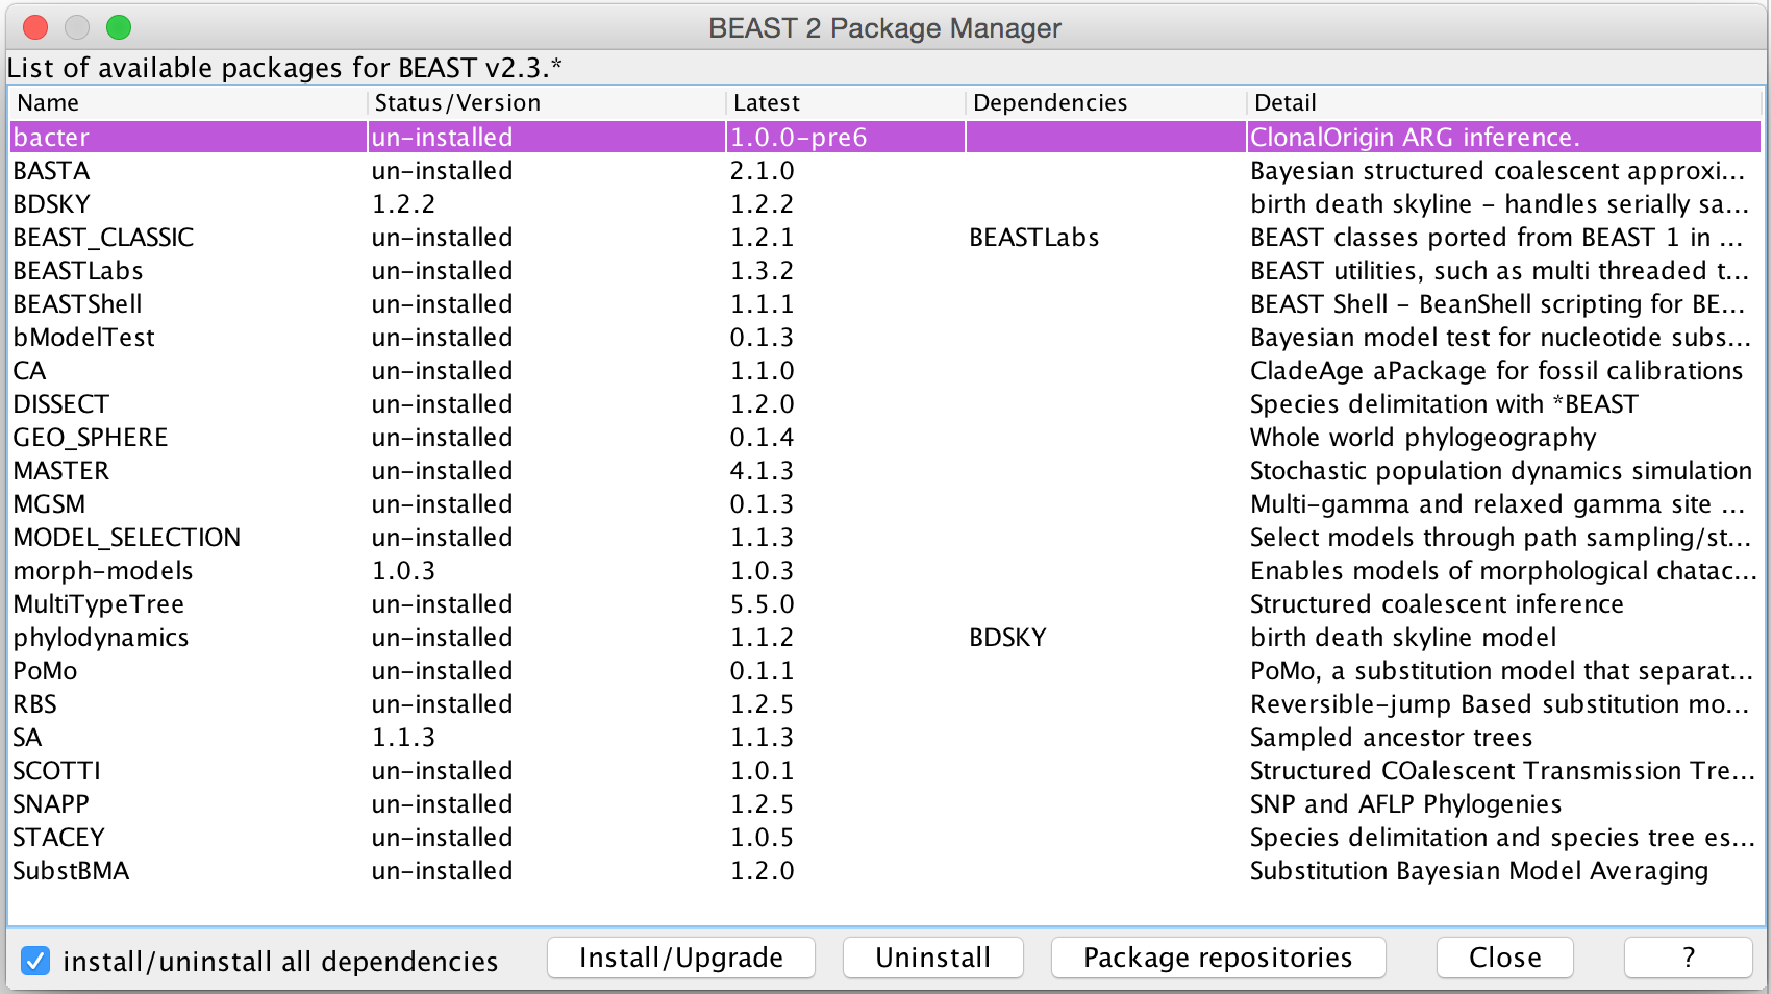
\includegraphics[width=5in]{figures/beast2_package_manager.pdf}}
\caption{\small The BEAST2 Package Manager.}
\label{packageManage}
\end{figure}

It is important to note that you only need to install a BEAST 2 package once, thus if you close BEAUti, you don't have to load \mi{SA} the next time you open the program. 
However, it is worth checking the package manager for updates to plug-ins, particularly if you update your version of BEAST 2.
\begin{framed}
Close the \mi{BEAST 2 Package Manager} and {\textcolor{red}{\underline{\bf restart BEAUti}}} to fully load the \mi{SA} package.
\end{framed}

\bigskip
\subsubsection{Import Alignments}

\begin{framed}
Navigate to the \mi{Partitions} window (you should already be here).
\end{framed}

Next we will load the alignment files for each of our genes. 
Note that separate loci can be imported as separate files or in a single NEXUS file with partitions defined using the \cl{ASSUMPTIONS} command.
\begin{framed}
Using the menu commands \mi{File\textrightarrow Import Alignment}, import the data files:\\ \ \ \ \ \cl{bears\_irbp\_fossils.nex} and \cl{bears\_cytb\_fossils.nex} 
\end{framed}

Now that the data are loaded into BEAUti, we can unlink the site models, link the clock models, link the trees and rename these variables.

\begin{framed}
Highlight both partitions (using shift$+$click) and click on \mi{Unlink Site Models} to assume different models of sequence evolution for each gene (the partitions are typically already unlinked by default).

Now click the \mi{Link Clock Models} button so that the two genes have the same relative rates of substitution among branches.

Finally click \mi{Link Trees} to ensure that both partitions share the same tree topology and branching times.
\end{framed}

It is convenient to rename some of the variables in the \mi{Partitions} window. 
By doing this, the parameters associated with each partition that are written to file are a bit more intuitively labeled.
\begin{framed}
Double click on the site model for the cytochrome b gene, it is currently called \cl{bears\_cytb\_fossils}. Rename this: \cl{cytb}. (Note that you may have to hit the return or enter key after typing in the new label for the new name to be retained.)

Do the same for the site model for the other gene, calling it \cl{irbp}.

Rename the clock model \cl{bearsClock}.

Rename the tree \cl{bearsTree}. [Figure \ref{importAlign}]
\end{framed}

\begin{figure}[h!]
\centering
\fbox{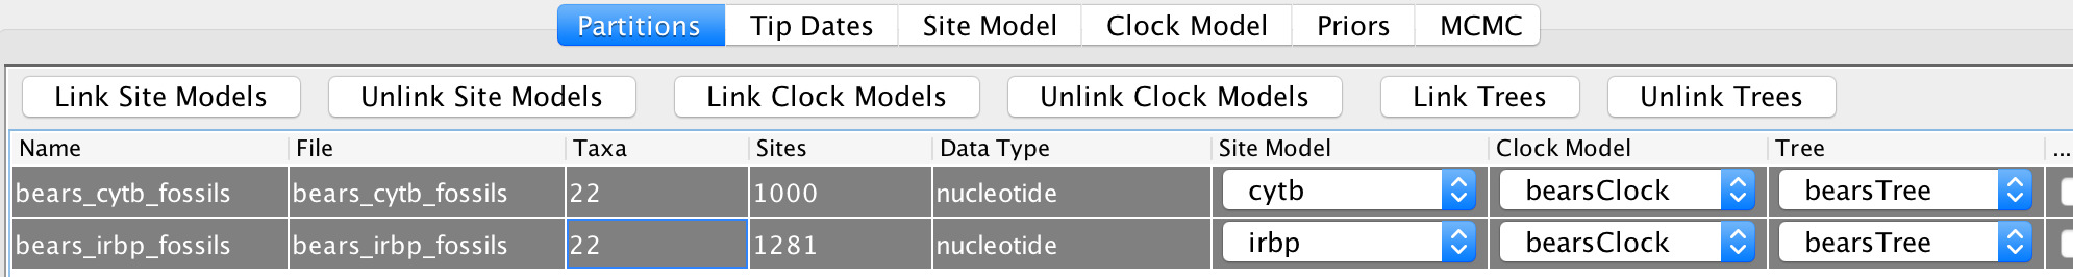
\includegraphics[width=6.25in]{figures/link_trees_partitions.pdf}}
\caption{\small The \mi{Partitions} window after unlinking the site models, linking the clock models, linking the trees, and renaming the XML variables.}
\label{importAlign}
\end{figure}

Figure \ref{importAlign} shows how the final \mi{Partitions} window should look.

\bigskip
\subsubsection{Set Tip Dates}

\begin{framed}
Navigate to the \mi{Tip Dates} panel.
\end{framed}

We must indicate that we have sequentially sampled sequences.
When performing an analysis without dated tips or any fossil information, you can skip this window, and BEAST will assume that all of your samples are contemporaneous.
\begin{framed}
Toggle on the \mi{Use tip dates} option.
\end{framed}

The next step involves specifying how the dates are oriented on the tree and the units they are in. We will indicate that the dates are in \mi{years}, even though they are in fact in units of \textit{millions of years}. 
This is because the units themselves are arbitrary and this scale difference will not matter.
Additionally, we will tell BEAUti that the zero time of our tree is the present and the ages we are providing are the number of years \mi{Before the present}. 
\begin{framed}
Change: \mi{Dates specified as: year Before the present} [Figure \ref{setTipDatesYears}]
\end{framed}
For some types of analyses, such as serially sampled viruses, the dates given are relative to some time in the past, thus this option is available as well.

\begin{figure}[h!]
\centering
\fbox{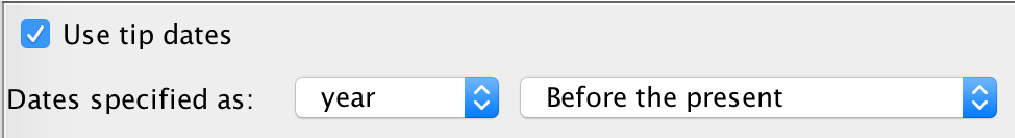
\includegraphics[width=3.5in]{figures/tip_dates_years.pdf}}
\caption{\small Specifying the units and reference point of the fossil dates.}
\label{setTipDatesYears}
\end{figure}

When inputing the dates for each tip species, one option is to enter each one by hand. 
This may be quite onerous if you have many fossils or many sequences sampled back in time.
Conveniently, these dates can be included in the taxon names so that BEAUti can easily extract them for us using the \mi{Auto-configure} option. 
\begin{framed}
Click on the \mi{Auto-configure} button.
\end{framed}
This will open a window where you can specify the pattern in the taxon names from which the tip ages can be extracted. 
Obviously, it's better to make this a fairly simple code that doesn't require multiple iterations of searches. 
Moreover, if this is straightforward, then you will be able to easily eliminate these dates when creating figures from your final summary tree.
\begin{framed}
Tell BEAUti to \mi{use everything} after the \mi{last} `\cl{\_}', then click \mi{OK}. [Figure \ref{guesTipDates}]
\end{framed}

\begin{figure}[h!]
\centering
\fbox{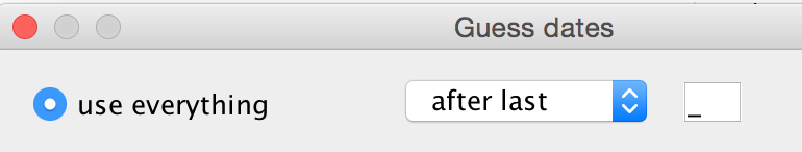
\includegraphics[width=2.5in]{figures/guess_tip_dates.pdf}}
\caption{\small Specify the text pattern in the taxon names that identifies the tip's age using the \mi{Guess dates} option.}
\label{guesTipDates}
\end{figure}

You should now see that the tip ages have been filled in for all of the fossil taxa and that the same age is listed in the \mi{Date} and \mi{Height} column for each species.


\bigskip
\subsubsection{Specify the Sites Model}

\begin{framed}
Navigate to the \mi{Site Model} window.
\end{framed}

The molecular sequence data sampled for each extant bear species are from two different genes: the mitochondrial cytochrome b gene (\cl{cytb}) and the nuclear interphotoreceptor retinoid-binding protein gene (\cl{irbp}).
We will partition these loci into two separate alignments and apply different models of sequence evolution to each one. 
For the \cl{cytb} gene, we will apply a general-time reversible model with homogeneous rates across sites: GTR.
For the nuclear gene \cl{irbp}, we will assume a 2-rate model where transitions and transversions happen at different rates, and that the rates vary across the alignment according to a mean-one gamma distribution: HKY+$\Gamma$.
\begin{framed}
Select the \cl{cytb} gene and change the \mi{Subst Model} to \mi{GTR}.

Toggle on \mi{estimate} for the \mi{Substitution Rate}. [Figure \ref{cytbSitesMod}]
\end{framed}
\begin{figure}[h!]
\centering
\fbox{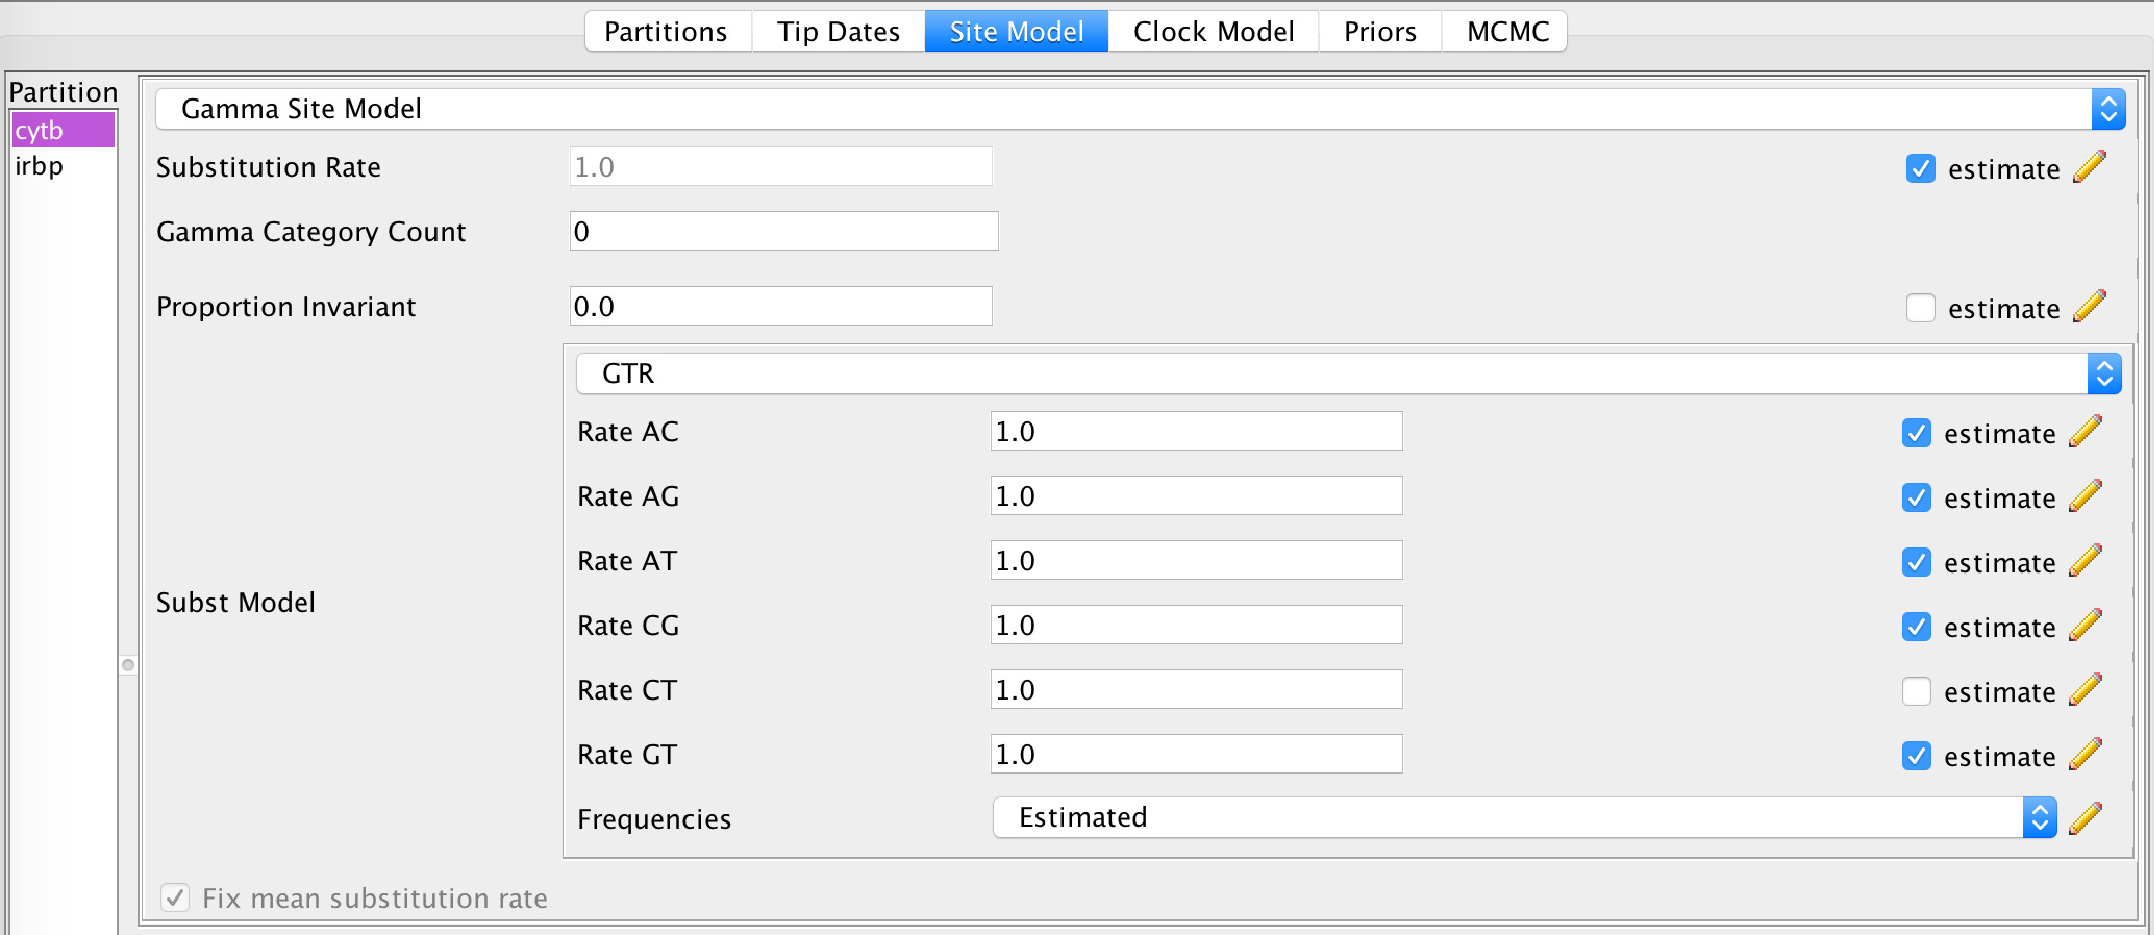
\includegraphics[width=4.5in]{figures/set_mito_sites_model.pdf}}
\caption{\small The fully specified site model for the \cl{cytb} gene: GTR. }
\label{cytbSitesMod}
\end{figure}

By changing the substitution model, we have now introduced additional parameters for the GTR exchangeability rates.
We will construct priors for these parameters later on. 

\begin{framed}
Select the \cl{irbp} gene and change the \mi{Subst Model} to \mi{HKY}.

To indicate gamma-distributed rates, set the \mi{Gamma Category Count} to 4.

Then switch the \mi{Shape} parameter to \mi{estimate}.

Toggle on \mi{estimate} for the \mi{Substitution Rate}. [Figure \ref{irbpSitesMod}]
\end{framed}

\begin{figure}[h!]
\centering
\fbox{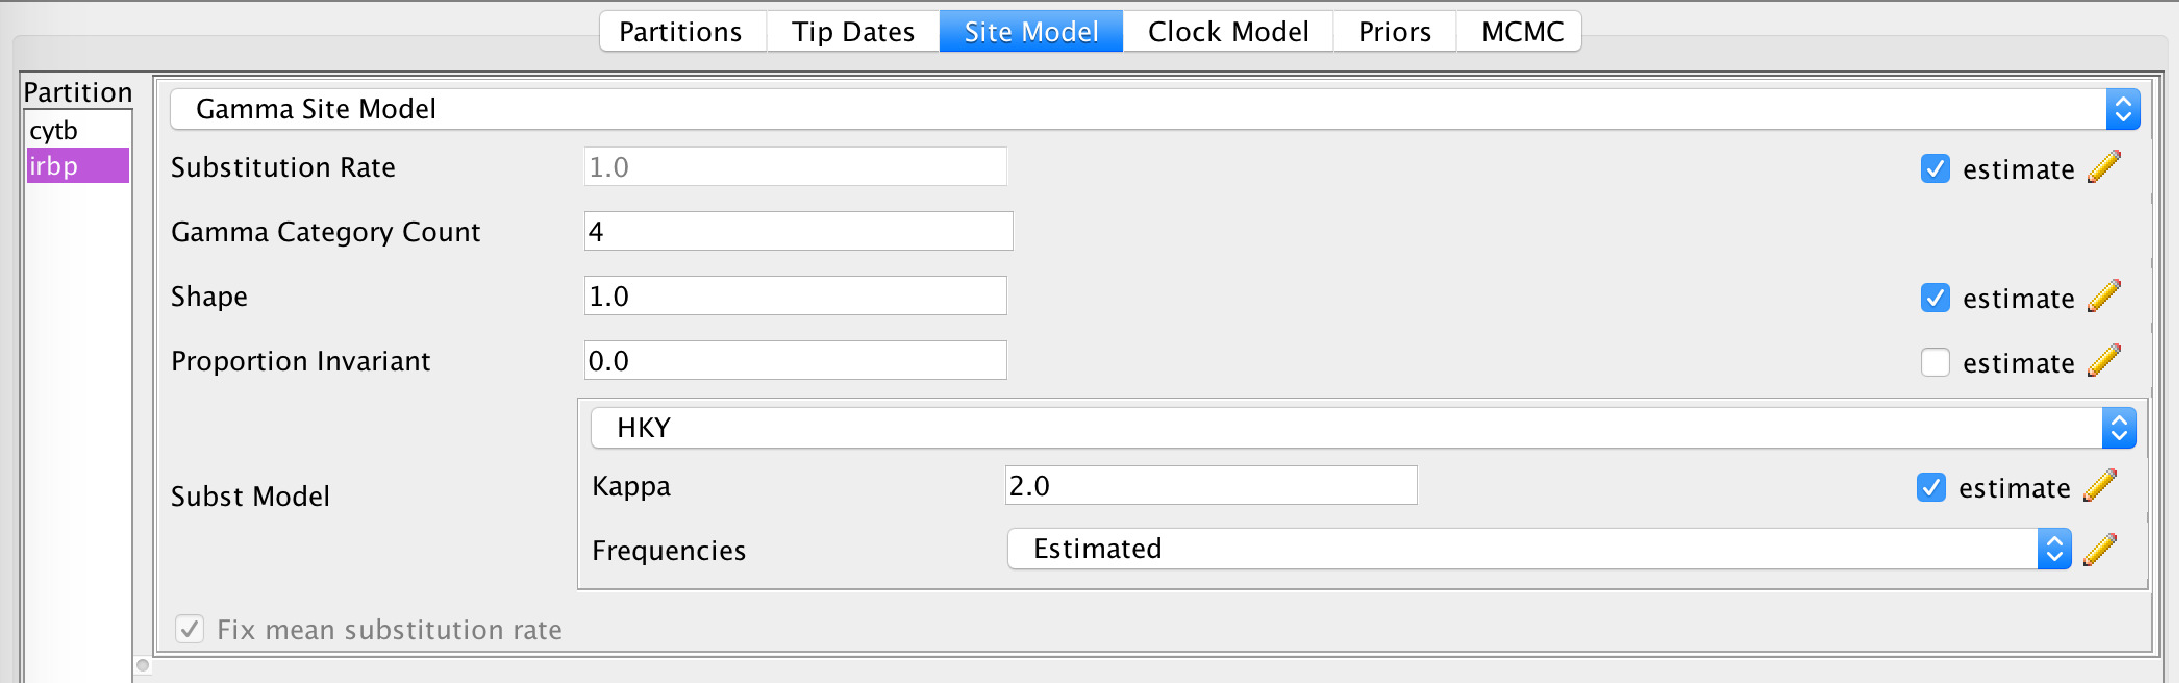
\includegraphics[width=4.5in]{figures/set_irbp_sites_model.pdf}}
\caption{\small The fully specified site model for the \cl{irbp} gene: HKY+$\Gamma$.}
\label{irbpSitesMod}
\end{figure}

Now both models are fully specified for the unlinked genes. Note that \mi{Fix mean substitution rate} is always specified and we also have indicated that we wish to \mi{estimate} the \mi{Substitution Rate} for each gene.
This means that we are estimating the \textit{relative} substitution rates for our two loci.



\bigskip
\subsubsection{The Clock Model}

\begin{framed}
Navigate to the \mi{Clock Model} window.
\end{framed}

Here, we can specify the model of lineage-specific substitution rate variation. The default model in BEAUti is the \mi{Strict Clock} with a fixed substitution rate equal to \cl{1}. Three models for relaxing the assumption of a constant substitution rate can be specified in BEAUti as well. The \mi{Relaxed Clock Log Normal} option assumes that the substitution rates associated with each branch are independently drawn from a single, discretized lognormal distribution \citep{drummond06}. Under the \mi{Relaxed Clock Exponential} model, the rates associated with each branch are exponentially distributed \citep{drummond06}. The \mi{Random Local Clock} uses Bayesian stochastic search variable selection to average over random local molecular clocks \citep{drummond10}. 
For this analysis we will use the uncorrelated, lognormal model of branch-rate variation.
\begin{framed}
Change the clock model to \mi{Relaxed Clock Log Normal}.
\end{framed}
The uncorrelated relaxed clock models in BEAST2 are discretized for computational feasibility. 
This means that for any given parameters of the lognormal distribution, the probability density is discretized into some number of discrete rate bins. 
Each branch is then assigned to one of these bins. 
By default, BEAUti sets the \mi{Number Of Discrete Rates} to \cl{-1}. This means that the number of bins is equal to the number of branches.

The fully specified \mi{Clock Model} assumes that the rates for each branch are drawn independently from a single lognormal distribution. 
The mean of the rate distribution will be estimated, thus we can account for uncertainty in this parameter by placing a prior distribution on its value.
Note that there is an option to \mi{Normalize} the average clock rate. We will leave this unchecked. 



\bigskip
\subsubsection{Priors on Parameters of the Site Models}

\begin{framed}
Navigate to the \mi{Priors} window.
\end{framed}



In the \mi{Priors} window, all of the  parameters and hyperparameters (and hyper-\textit{hyper}parameters, etc.) specific to the models defined in the \mi{Site Model} and \mi{Clock Model} windows are listed. 
Here you can set up the prior distributions on these parameters, as well as define calibration nodes and calibration densities and specify a tree model. 
One convenient feature of BEAUti is that the list of parameters changes dynamically as you change the models. Thus, if you missed a step along the way, you would notice at this point because something might be missing here. For example, if you did not change the substitution mode for \cl{cytb} from \mi{JC69} to \mi{GTR} in the \mi{Site Model} window, then you would not see the exchangeability rates and base frequency parameters listed for \cl{cytb}. 
[Figure \ref{fig:priorPanel}]




\begin{figure}[h!]
\centering
\fbox{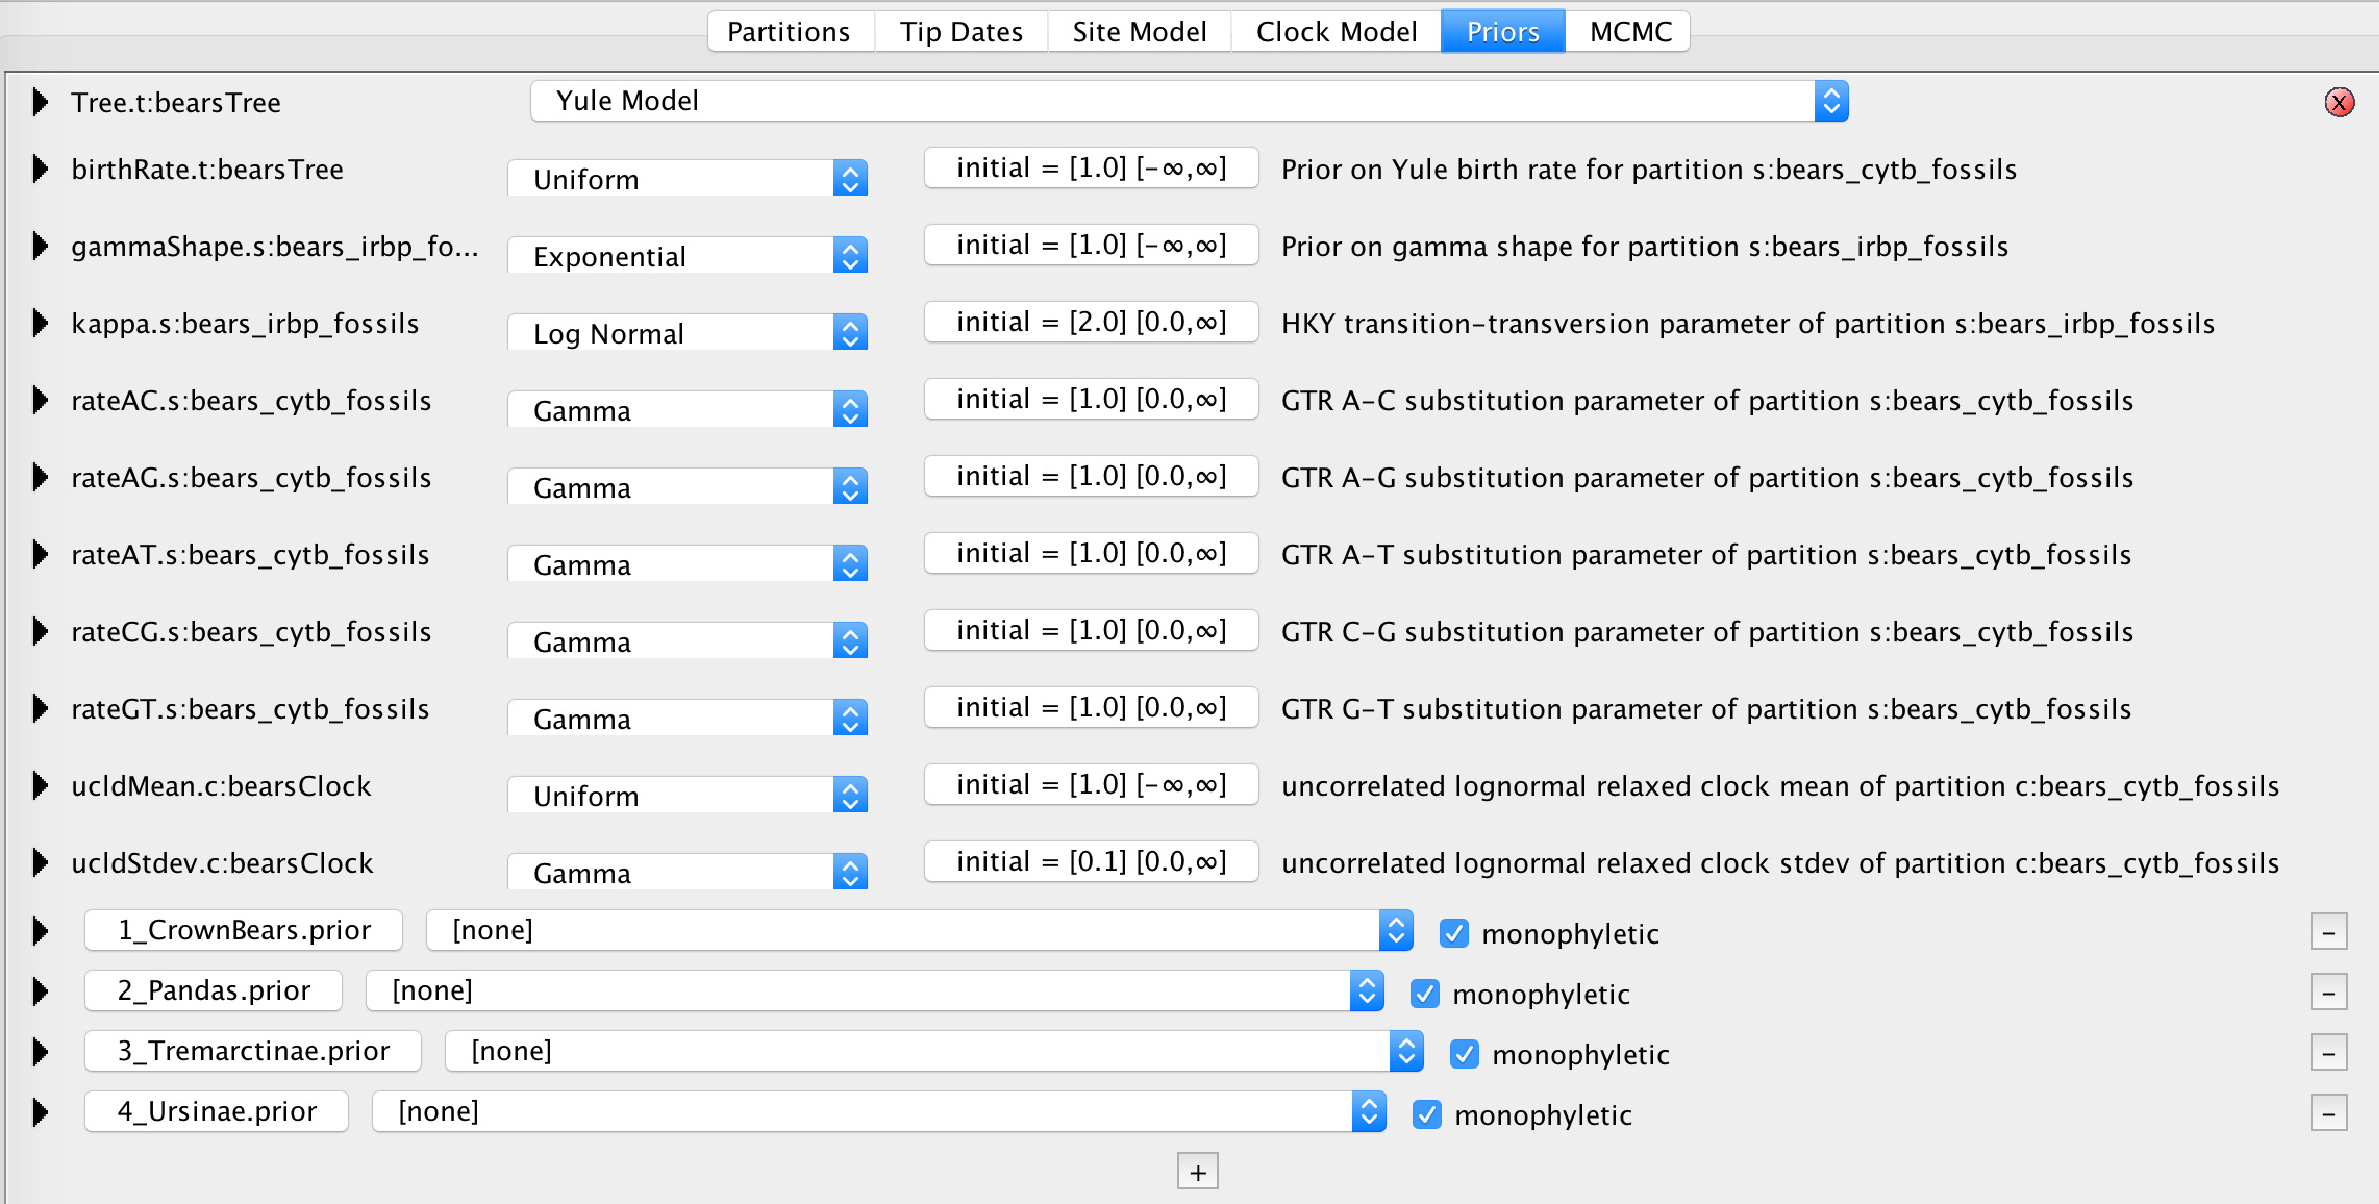
\includegraphics[width=6.5in]{figures/priors_panel_initial.pdf}}
\caption{\small The \mi{Priors} window with default (unmodified) settings.}
\label{fig:priorPanel}
\end{figure}

In the \mi{Priors} panel we will begin by specifying priors for the parameters associated with the sites models.
Since we partitioned the two genes, there are parameters for the two different models: 
\begin{itemize}[noitemsep,topsep=0pt,parsep=0pt,partopsep=0pt]
\item \cl{cytb}: exchangeability rates for the GTR model (\mi{rateAC.s:cytb}, \mi{rateAG.s:cytb}, $\ldots$)
\item \cl{irbp}: the transition-transversion rate ratio (\mi{kappa.s:irbp}) and the shape parameter of the gamma distribution on site rates (\mi{gammaShape.s:irbp})
\end{itemize}
Note that the base frequencies for each of these models are not listed in the \mi{Priors} window, though they are estimated.

We will keep the default priors for the HKY model on the evolution of \cl{irbp}. 
The default gamma priors on the GTR exchangeability rates for the \cl{cytb} gene place a lot of prior density on very small values.
For some datasets, the sequences might not be informative for some of the rates, consequentially the MCMC may propose values very close to zero and this can induce long mixing times. 
Because of this problem, we will alter the gamma priors on the exchangeability rates. 
For each one, we will keep the expected values as in the default priors.
The default priors assume that transitions (A$\leftrightarrow$G or C$\leftrightarrow$T) have an expected rate of 1.0. 
Remember that we fixed the parameter \mi{rateCT} to equal 1.0 in the \mi{Site Model} window, thus this parameter isn't in the \mi{Priors} window. 
For all other rates, transversions, the expected value of the priors is lower: 0.5.
In BEAST, the gamma distribution is parameterized by a shape parameter (\mi{Alpha}) and a scale parameter (\mi{Beta}). 
Under this parameterization, expected value for any gamma distribution is: $\mathbb{E}(x) = \alpha\beta$.
To reduce the prior density on very low values, we can increase the shape parameter and then we have to adjust the scale parameter accordingly.

\begin{framed}
Begin by changing the gamma prior on the transition rate \mi{rateAG.s:cytb}. Clicking on the $\blacktriangleright$ next to this parameter name to reveal the prior options. Change the parameters: \mi{Alpha} = \cl{2} and \mi{Beta} = 0.5. [Figure \ref{screenGTRprior}, bottom]

Then change all of the other rates: \mi{rateAC.s}, \mi{rateAT.s}, \mi{rateCG.s}, \mi{rateGT.s}. For each of these, change the parameters to:  \mi{Alpha} = \cl{2} and \mi{Beta} = 0.25. [Figure \ref{screenGTRprior}, top]
\end{framed}

\begin{figure}[h!]
\centering
\fbox{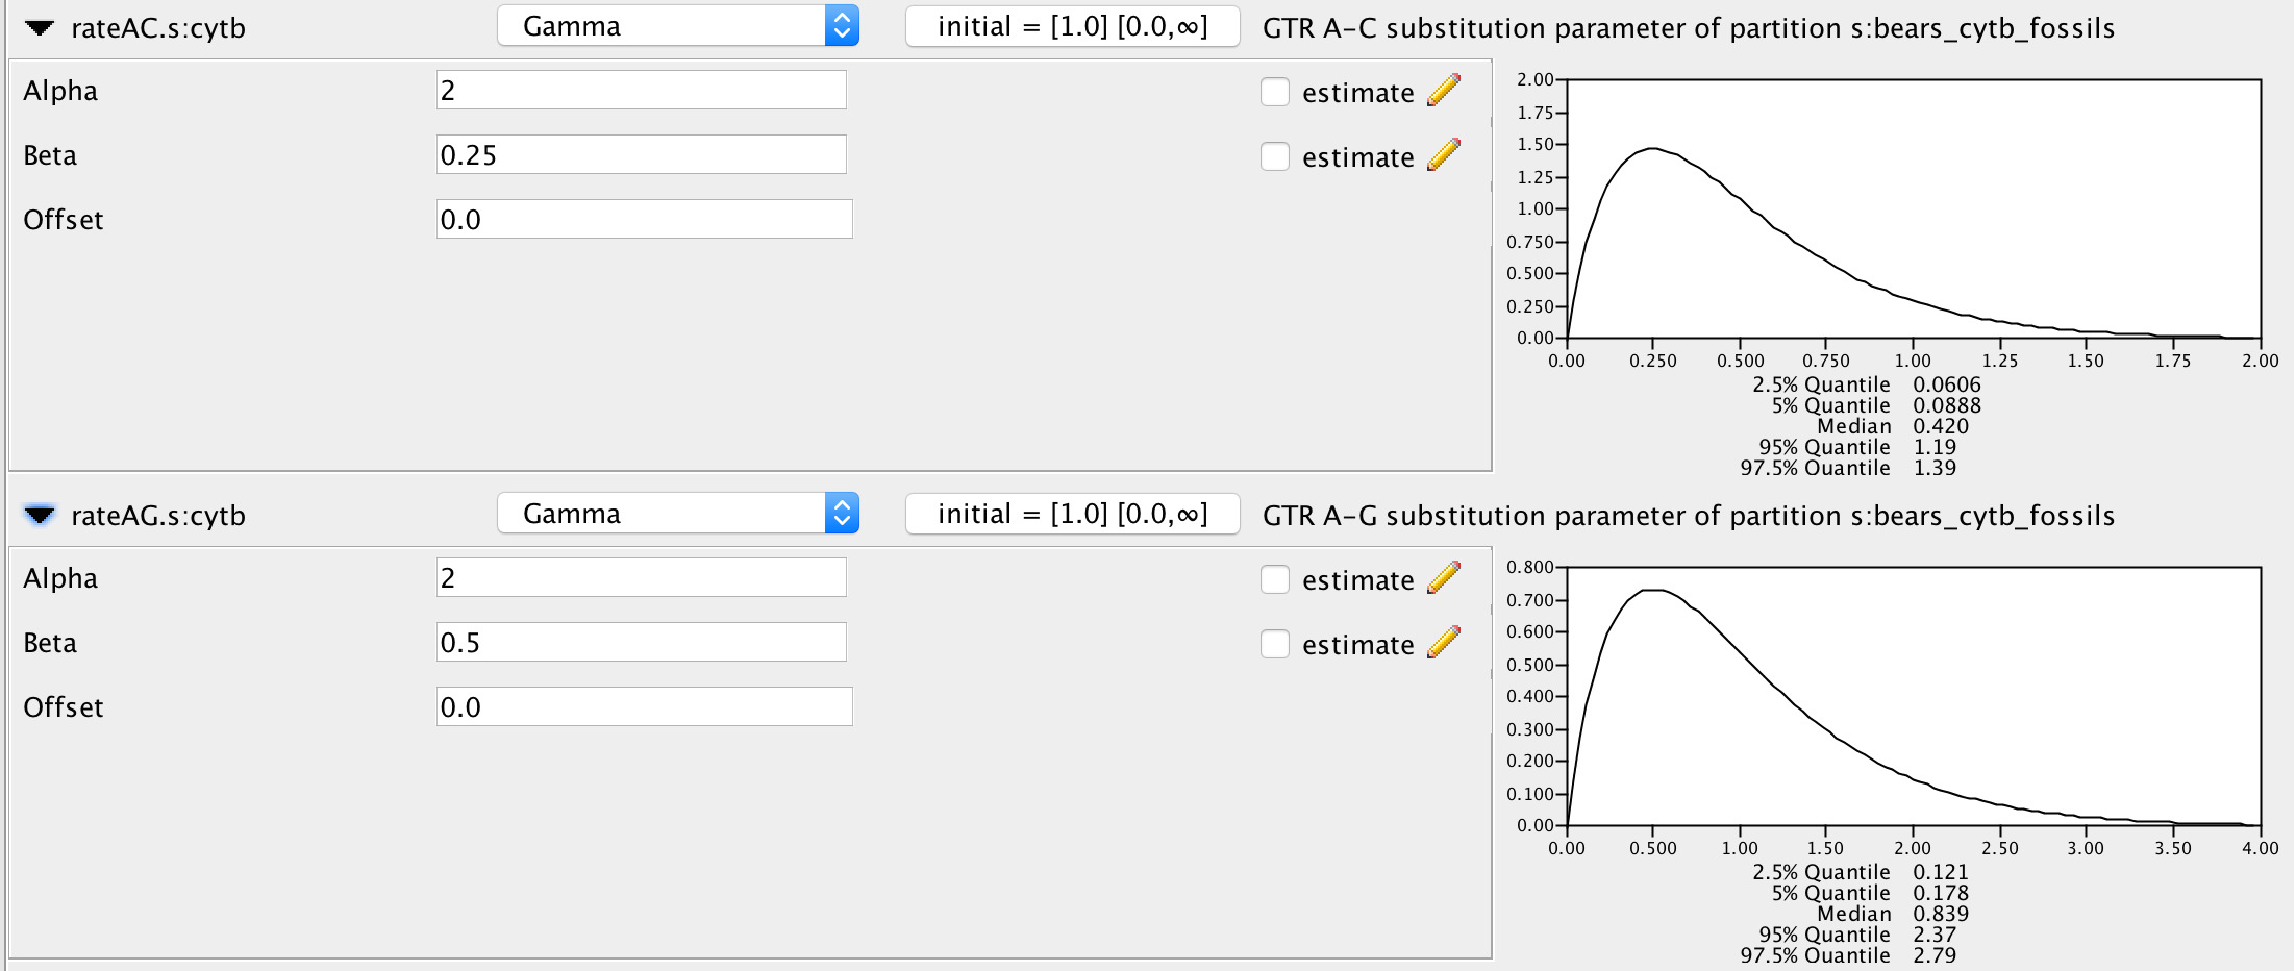
\includegraphics[width=6.5in]{figures/priors_on_GTR_rates.pdf}}
\caption{\small Gamma prior distributions on two of the five relative rates of the GTR model. }
\label{screenGTRprior}
\end{figure}



\bigskip
\subsubsection{Priors for the Clock Model}


Since we are assuming that the branch rates are drawn from a lognormal distribution, this induces two hyperparameters: the mean and standard deviation (\mi{ucldMean.c} and \mi{ucldStdev.c} respectively). 
By default, the prior distribution on the \mi{ucldMean.c} parameter is an improper, uniform distribution on the interval ($0,\infty$). 
Note that this type of prior is called improper because the prior density of a \textit{uniform} distribution with infinite bounds does not integrate to $1$. Although improper priors can sometimes lead to proper posterior distributions, they may also have undesired effects and cause problems with mixing and convergence. 
\begin{framed}
Reveal the options for the prior on \mi{ucldMean.c} by clicking on the $\blacktriangleright$. Change the prior density to an \mi{Exponential} with a mean of \cl{10.0}. [Figure \ref{setPriorUCLD}]
\end{framed}
%%% More info needed here

\begin{figure}[h!]
\centering
\fbox{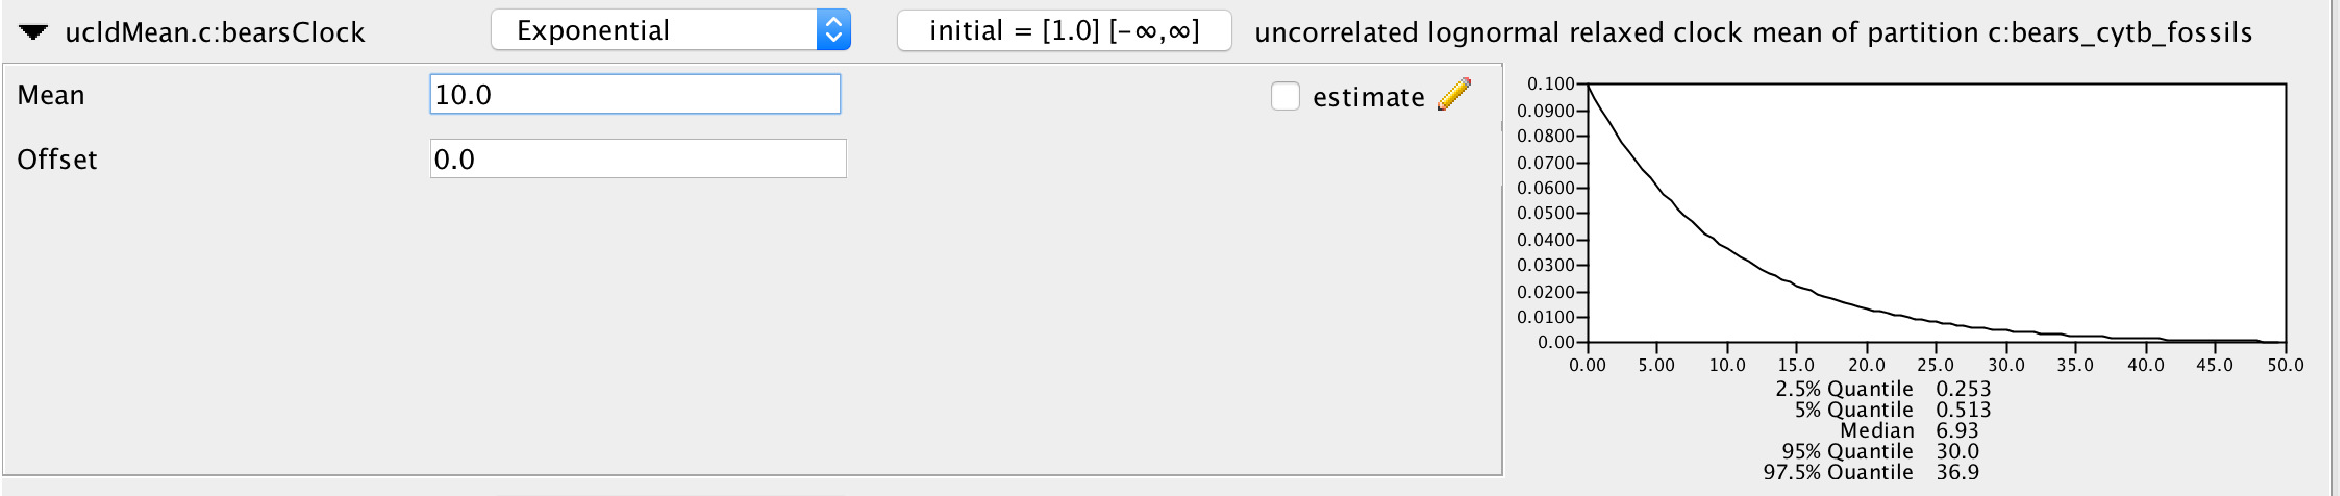
\includegraphics[width=6.5in]{figures/set_exp_prior_on_ucldmean.pdf}}
\caption{\small The exponential prior distribution on the mean of the log normal relaxed clock model.}
\label{setPriorUCLD}
\end{figure}

The other parameter of our relaxed-clock model is, by default assigned a gamma prior distribution. 
However, we have a strong prior belief that the variation in substitution rates among branches is low, since some previous studies have indicated that the rates of molecular evolution in bears is somewhat clock-like \citep{krause2008}. 
Thus, we will assume an exponential prior distribution with 95\% of the probability density on values less than 1 for the \mi{ucldStdev.c} parameter.
\begin{framed}
Reveal the options for the prior on \mi{ucldStdev.c} by clicking on the $\blacktriangleright$. Change the prior density to an \mi{Exponential} with a mean of \cl{0.3337}. [Figure \ref{setPriorUCLDSTDV}]
\end{framed}

\begin{figure}[h!]
\centering
\fbox{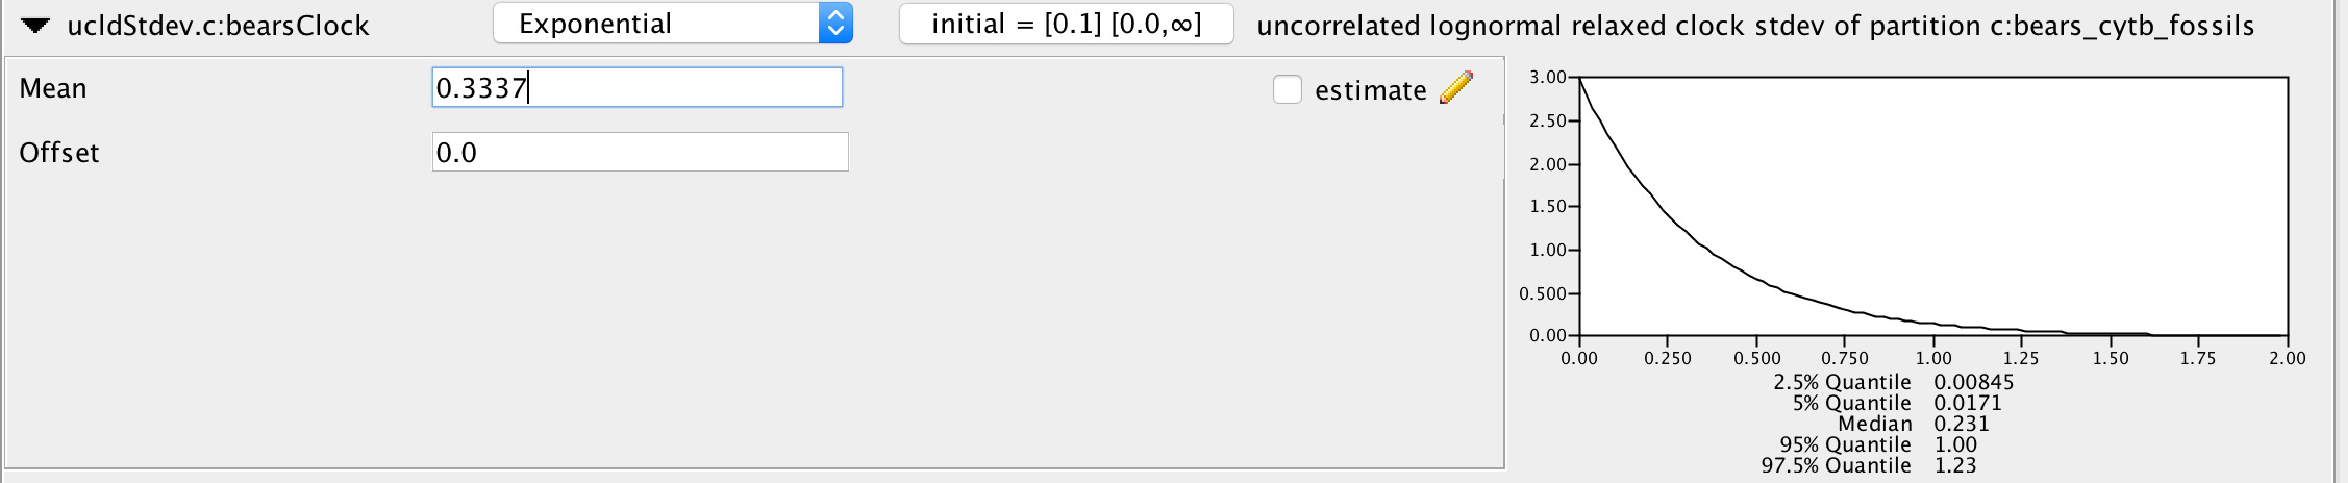
\includegraphics[width=6.5in]{figures/exp_prior_on_ucldstdv.pdf}}
\caption{\small The exponential prior distribution on the standard deviation of the log normal relaxed clock model.}
\label{setPriorUCLDSTDV}
\end{figure}


\bigskip
\subsubsection{The Tree Prior}

Next we will specify the prior distribution on the tree topology and branching times. 
You should notice an error notification (a red circle with an ``X'' in it) in the \mi{Priors} panel to the left of \mi{Tree.t:bearsTree} (Figure \ref{fig:priorPanel}). 
If you mouse over this notification, you will se a message telling you that the default \mi{Yule Model} is not appropriate for non-contemporaneous tips and that you must choose a different tree prior.
Thus, here is where we specify the \textit{fossilized birth-death process}.
\begin{framed}
Change the tree model for \mi{Tree.t:bearsTree} to \mi{Fossilized Birth Death Model}. %[Figure \ref{selectFBD}]

Reveal the options for the prior on \mi{Tree.t} by clicking on the $\blacktriangleright$. 
\end{framed}
%
%\begin{figure}[h!]
%\centering
%\fbox{\includegraphics[width=3.5in]{figures/select_FBD.eps}}
%\caption{\small The tree priors available for specification in BEAUti.}
%\label{selectFBD}
%\end{figure}

\textsc{Origin Time} --- In Section \ref{FBDSection}, the parameters of the FBD model are given. 
Remember that this model, like any branching process (i.e., constant rate birth-death, Yule) can be conditioned on either the origin time or the root age.
Depending on the available prior information or the type of data available, it makes sense to condition on one or the other (but not both, obviously). 
If you know that all of the fossils in your dataset are \textit{crown} fossils---descendants of the MRCA of all the extant taxa---and you have some prior knowledge of the age of the clade, then it is reasonable to condition the FBD on the root. 
Alternatively, if the fossils in your analysis are stem fossils, or can only reliably be assigned to your total group, then it is appropriate to condition on the origin age.

For this analysis, we have several bear fossils that are considered stem fossils, thus we will condition on the origin age. 
Previous studies \citep{dosReis2012} estimated an age of approximately 45.5 My for the MRCA of seals and bears. 
We will use this time as a starting value for the origin. 
\begin{framed}
Set the starting value of the \mi{Origin} to 45.5 and specify that this parameter will be estimated by checking the \mi{estimate} box. (You may have to expand the width of the BEAUti window to see the check-boxes for these parameters.) [Figure \ref{fullFBD}]
\end{framed}

\begin{figure}[h!]
\centering
\fbox{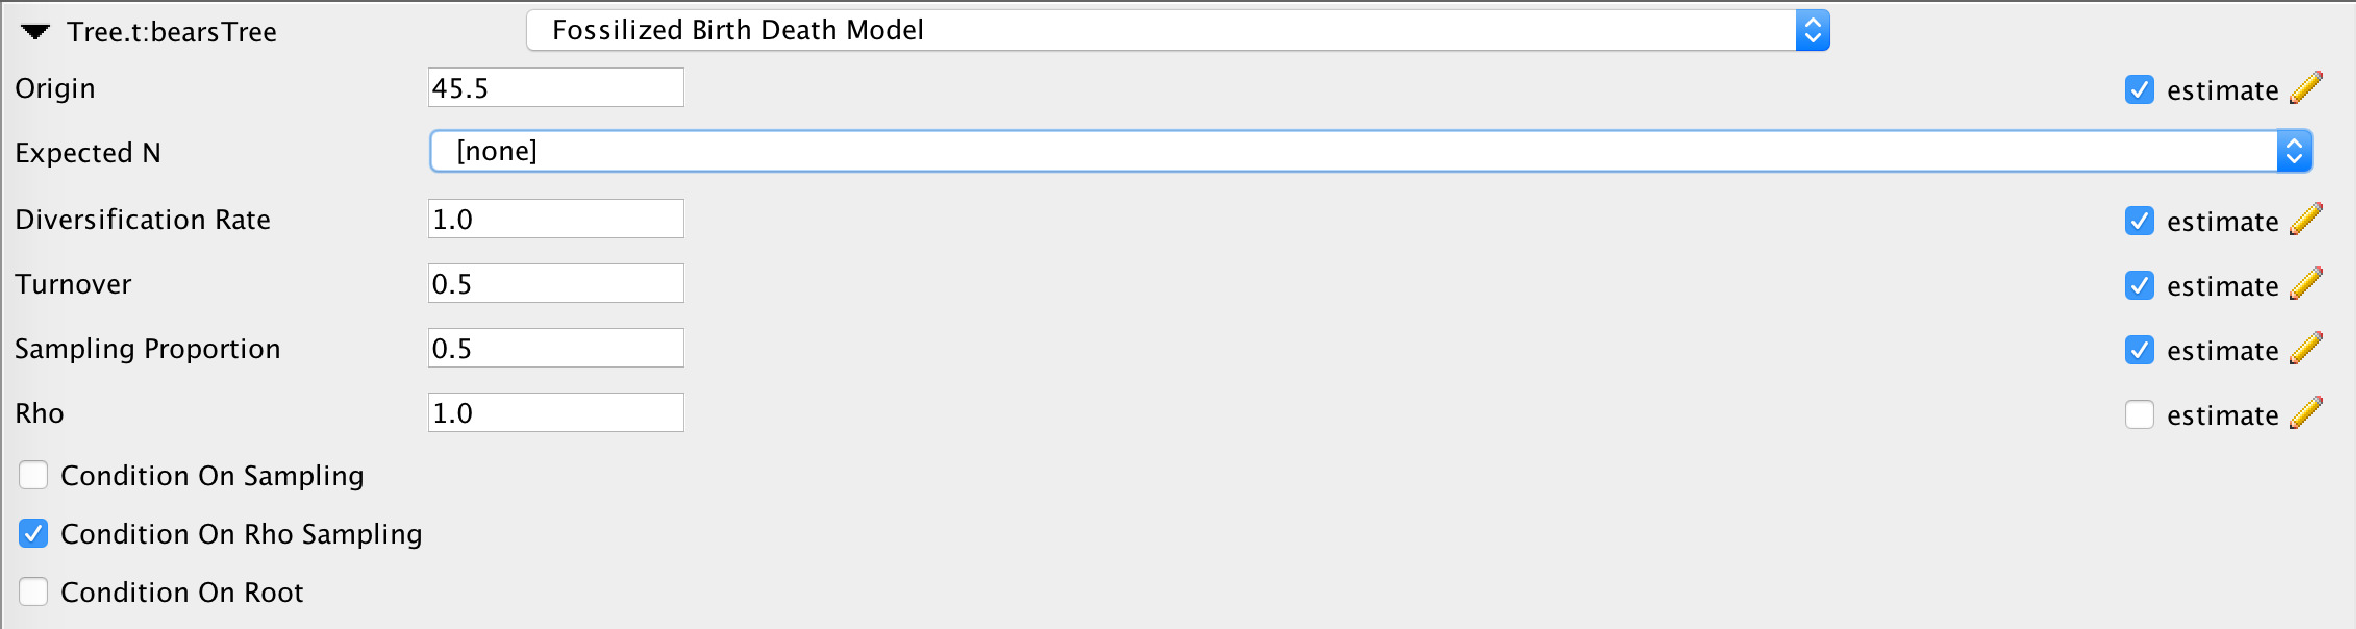
\includegraphics[width=6.5in]{figures/specified_FBD_model.pdf}}
\caption{\small The initial values and conditions for the fossilized birth-death process \citep{stadler10,heath2013fossilized,gavryushkina2014}}
\label{fullFBD}
\end{figure}

Since we are estimating the origin parameter, we must assign a prior distribution to it (unless we wish to keep the default Uniform(0,$\infty$) prior).
We will assume that the origin time is drawn from a lognormal distribution with an expected value (mean) equal to 45.5 My and a standard deviation of 1.0.
\begin{framed}
Reveal the options for the prior on \mi{originFBD.t} by clicking on the $\blacktriangleright$.

Change the prior distribution to \mi{Log Normal}.

Check the box marked \mi{Mean In Real Space} and set the mean \mi{M} equal to \cl{8.5} and the standard deviation \mi{S} to \cl{1.0}.

Set the \mi{Offset} of the lognormal distribution to  equal the age of the oldest fossil: \cl{37.0}. [Figure \ref{priorOrigin}]
\end{framed}
\begin{figure}[h!]
\centering
\fbox{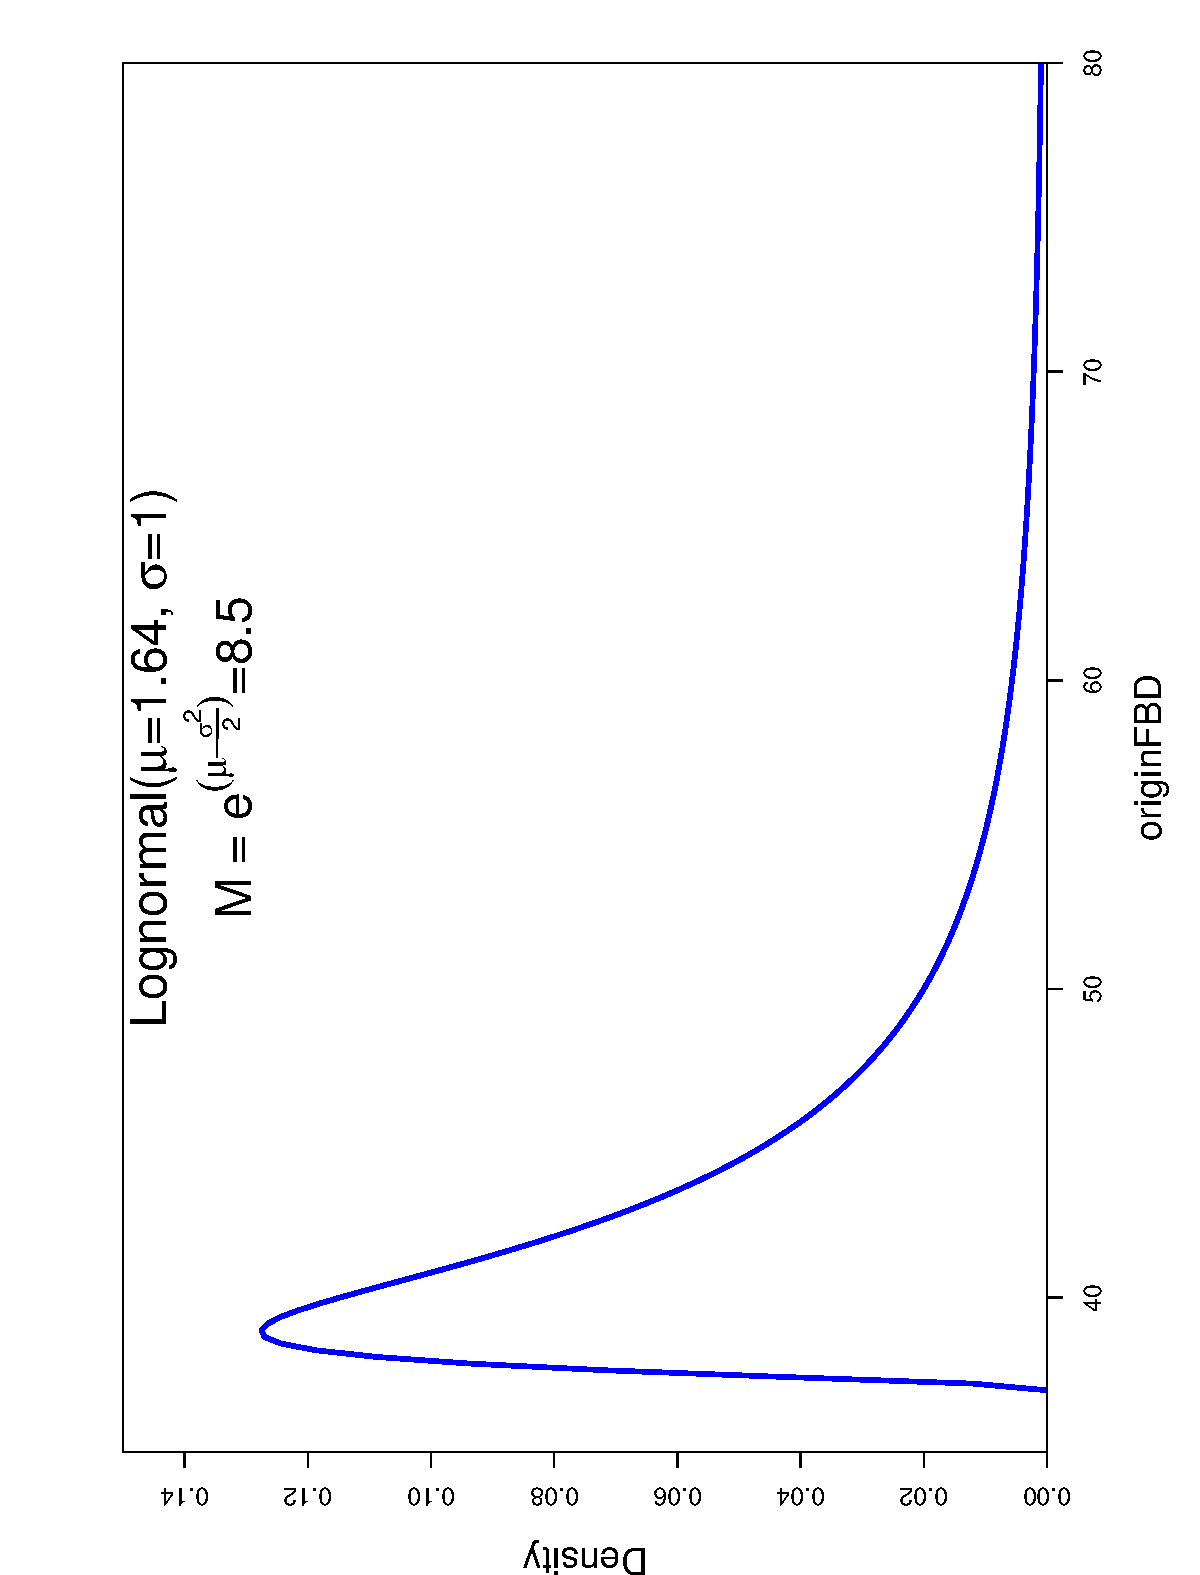
\includegraphics[width=2.5in,angle=-90]{figures/ln_den.pdf}}
\caption{\small The lognormal prior distribution on the origin time.}
\label{priorOrigin}
\end{figure}

Notice that the options for the \mi{Log Normal} prior distribution allow you to specify \mi{Mean in Real Space}. If you choose this option, then the mean value you enter is the expected value of the lognormal distribution. 
We used this option above to specify an expected value of 8.5 My.
You will create the exact same prior distribution if you uncheck the \mi{Mean in Real Space} option and enter the location parameter $\mu$ of the distribution and give it a value of \cl{1.640066}.
It is important that you are very careful when specifying these parameters. If, for example, \mi{Mean in Real Space} was not checked and you provided a value of \cl{8.5} for \mi{M}, then your calibration prior would be extremely diffuse, with a \textit{mean} value of 8,140.084!


\textsc{Diversification Rate} --- In Section \ref{FBDSection}, we discussed that the diversification rate is: $d = \lambda-\mu$. 
Generally, we think that this value is fairly small, particularly since we have few extant species and many fossils. 
Therefore, an exponential distribution is a reasonable prior for this parameter as it places the highest probability on zero. 
For this analysis we will assume $d\sim$ Exponential(1.0). 
The exponential distribution's only parameter is called the \textit{rate} parameter (denoted $\nu$) and it controls both the mean and variance of the distribution (here $\nu=1$).
The mean of an exponential distribution is the inverse of the rate: $\mathbb{E}(d) = \nu^{-1} = 1$.
Importantly, in BEAUti/BEAST, when specifying an exponential prior, you provide the \textit{mean} and not the rate parameter.
\begin{framed}
Reveal the options for the prior on \mi{diversificationRateFBD.t} by clicking on the $\blacktriangleright$.

Change the prior distribution to \mi{Exponential} with a \mi{Mean} equal to \cl{1.0}. [Figure \ref{priorSampProp}A]
\end{framed}


\begin{figure}[h!]
\centering
\fbox{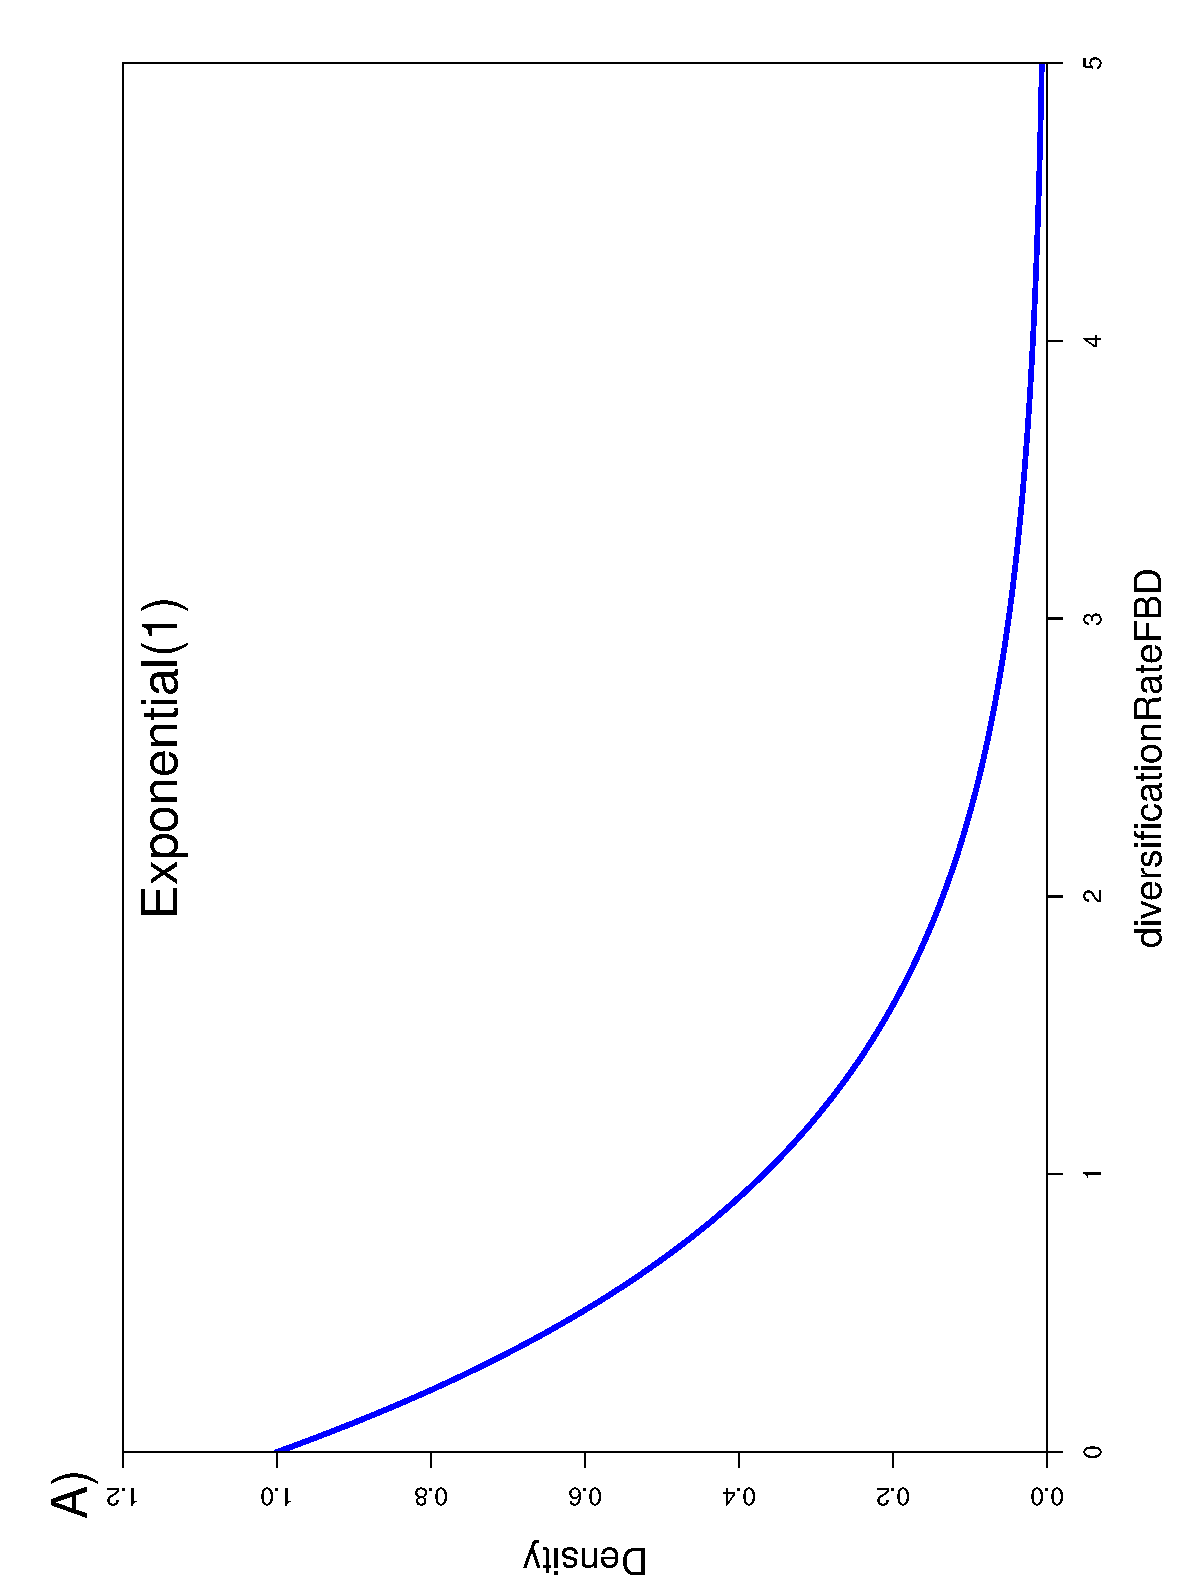
\includegraphics[width=2.5in,angle=-90]{figures/exp_den.pdf}\hspace{2mm}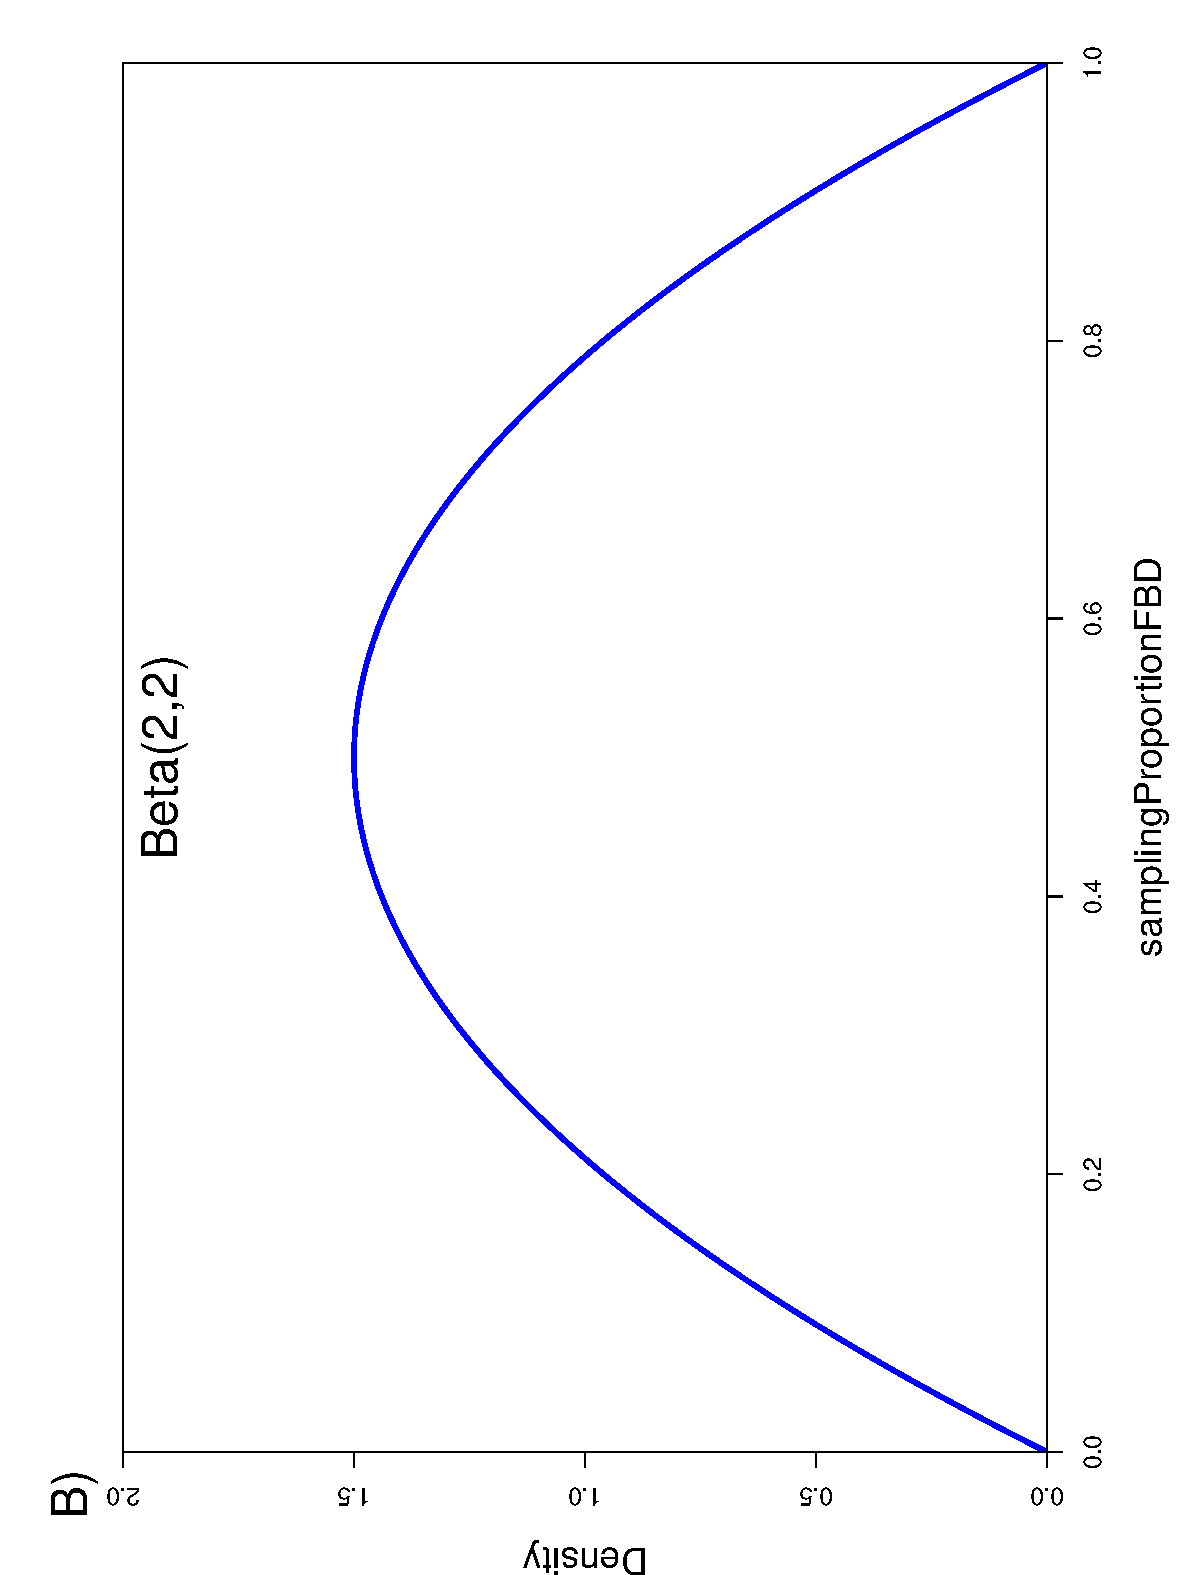
\includegraphics[width=2.5in,angle=-90]{figures/beta_den.pdf}}
\caption{\small Prior distributions on FBD parameters. (A) An exponential prior with a mean of 1 describes the distribution on the diversification rate ($d=\lambda-\mu$). (B) The sampling proportion is the probability of observing a fossil prior to the lineage extinction ($s = \psi /(\mu+\psi)$). Because this parameter is on the interval [0,1], we assume a beta prior density with $\alpha=\beta=2$.}
\label{priorSampProp}
\end{figure}



\textsc{Sampling Proportion} --- The sampling proportion is the probability of observing a lineage as a fossil before that lineage goes extinct. 
This parameter is a function of the extinction rate ($\mu$) and fossil recovery rate ($\psi$): $s=\psi / (\mu+\psi)$.
Let's say that we have prior knowledge that this parameter is approximately equal to 0.5, and that we wish extreme values (very close to 0 or 1) to have low probability. 
This prior density can be described with a beta distribution.
The \href{http://en.wikipedia.org/wiki/Beta_distribution}{beta distribution} is a probability density over values between 0 and 1 and is parameterized by two values, called $\alpha$ and $\beta$. 
A beta distribution with $\alpha=\beta=1$ is equivalent to a uniform distribution between 0 and 1.
By changing the parameters, we can assign higher probability to values closer to 1 or 0. 
The mean of the beta distribution on $s$ is: $\mathbb{E}(s) = \frac{\alpha}{\alpha+\beta}$.
Thus, if $\alpha=\beta$, then $\mathbb{E}(s) = 0.5$.
For this prior we will set $\alpha=\beta=2$.
\begin{framed}
Reveal the options for the prior on \mi{samplingProportionFBD.t} by clicking on the $\blacktriangleright$.

Change the prior distribution to \mi{Beta} with \mi{Alpha} equal to \cl{2.0} and \mi{Beta} equal to \cl{2.0}. [Figure \ref{priorSampProp}B]
\end{framed}

%The remaining parameters of the FBD model include the probability of sampling an extant tip (\mi{Rho} or $\rho$) and the \mi{Turnover} (\mi{turnoverFBD} or $r=\mu/\lambda$).
\textsc{The Proportion of Sampled Extant Species} --- The parameter $\rho$ (\mi{Rho}) represents the probability of sampling a tip in the present. 
For most birth-death processes, it is helpful to be able to fix or place a very strong prior on one of the parameters ($\lambda, \mu,\rho,\psi$) because of the strong correlations that exist among them. 
Typically, we may have the most prior knowledge about the proportion of sampled extant species ($\rho$). 
The diversity of living bears is very well understood and we know that there are only 8 species around today.
Since we have sequence data representing each species, we can then fix $\rho=1$, thus we do not need to specify a prior for this parameter.

\textsc{Turnover} --- This parameter represents the relative rate of extinction: $r = \mu/\lambda$.
For most implementations of the birth-death process, we assume that $\mu < \lambda$, thus this parameter is always $r < 1$. 
Large values of $r$ that are close to 1.0, indicate high extinction, and values close to 0, indicate very little extinction.
It is more challenging to define an appropriate prior for the turnover parameter and we will simply assume that all values on the interval [0,1] have equal probability. 
Thus, we can leave the default prior, a Uniform(0,1), on this parameter.

\bigskip
\subsubsection{Creating Taxon Sets}

Since some of the relationships of the fossil and living bears are well understood (from previous analyses of molecular and morphological data), we can incorporate this prior information by creating monophyletic taxon sets in BEAUti.
If we do not impose any phylogenetic structure on the fossil lineages, they will have equal probability of attaching to any branch in the tree.
Given that previous studies have provided information about the relationships of fossil bears, we can limit the MCMC to only sample within the known groups.
For example, morphological analysis of fossil taxa place the sequoias \textit{Kretzoiarctos beatrix} and several others in the subfamily Ailuropodinae, which includes pandas.
Thus, if we create a monophyletic taxon set containing these taxa (\textit{Ailuropoda melanoleuca, Indarctos vireti, Indarctos arctoides, Indarctos punjabiensis, Ailurarctos lufengensis, Agriarctos spp., Kretzoiarctos beatrix}) the prior probability that \textit{K.~beatrix} will attach to any lineage outside of this group is equal to 0.

There are five distinct clades within the phylogeny of bears that we can define (see Figure \ref{fig:clades}), and four out of five of these clades are defined as taxon sets in one of the nexus files containing our sequences (\cl{bears\_cytb\_fossils.nex}).
The taxa represented in our dataset are in the \textit{total group} of bears. This includes all of the fossils that diverged before the most-recent-common-ancestor (MRCA) of all \textit{living} bears. 
These early diverging fossils are \textit{stem} lineages.


%Four out of five of the taxon sets needed for this analysis have been specified in one of the nexus files containing our sequences (\cl{bears\_cytb\_fossils.nex}).
The first taxon set is the crown bears shown in Figure \ref{figtaxset1}. 
The crown bears include all living species of bears and all the fossils that are descended from the MRCA of living taxa (node 1 in Figure \ref{fig:clades}).
The MRCA of all crown bears and stem lineages is represented by the root node of our tree (node R in Figure \ref{fig:clades}).
We do not have to specify a taxon set for the root node.
%Let's start by creating a taxon set representing the MRCA of crown bears (node 1 in Figure \ref{fig:clades}).


\begin{figure}[h!]
\centering
\fbox{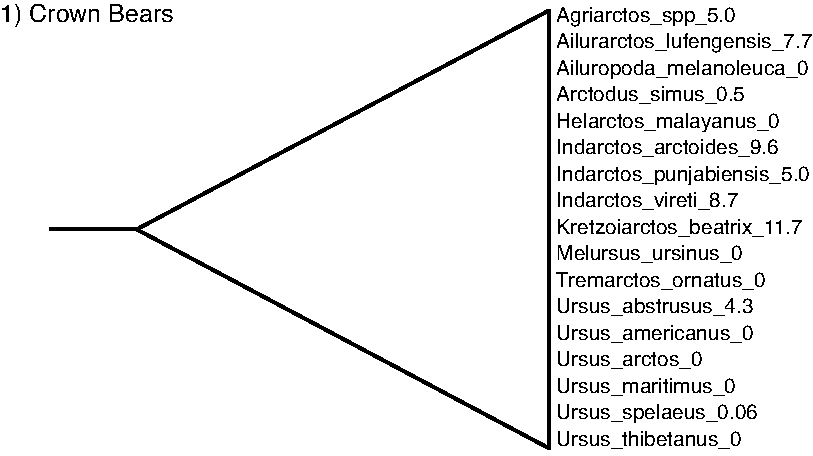
\includegraphics[width=3in]{figures/ts_crown_urs.pdf}}
\caption{\small The species belonging to the Crown Bears clade.}
\label{figtaxset1}
\end{figure}

\begin{framed}
If you view the file \cl{bears\_cytb\_fossils.nex} in your text editor, you will see the four taxon sets defined in the \cl{sets} block of the \cl{NEXUS} file.

\begin{lstlisting}
begin sets;
taxset 1_CrownBears = Agriarctos_spp_5.0 ... Ursus_thibetanus_0;
taxset 2_Pandas = Agriarctos_spp_5.0 ... Kretzoiarctos_beatrix_11.7;
taxset 3_Tremarctinae = Arctodus_simus_0.5 Tremarctos_ornatus_0;
taxset 4_Ursinae = Helarctos_malayanus_0 ... Ursus_thibetanus_0;
end;
\end{lstlisting}

When you have a \cl{taxset} in your data file, this creates a defined clade in BEAUti that is constrained to be monophyletic.

You can also open the BEAUti taxon set for the crown bears by clicking the  \mi{1\_CrownBears.prior} button. This will bring up the \mi{Taxon set editor} where you can modify this taxon set (don't do that, though). [Figure \ref{screentaxset1}]
\end{framed}

\begin{figure}[h!]
\centering
\fbox{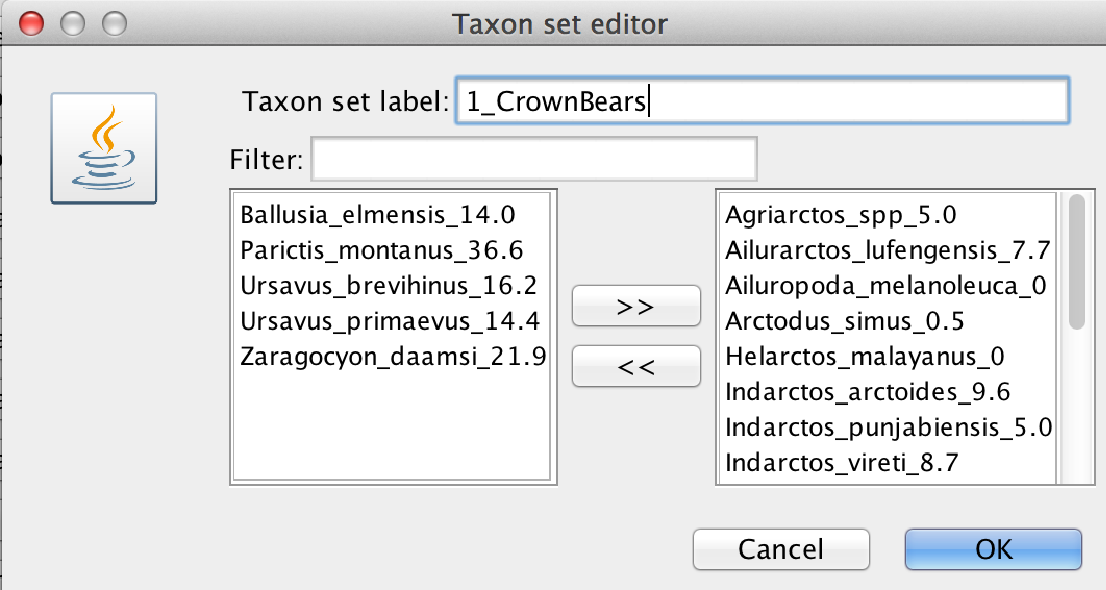
\includegraphics[width=4in]{figures/ts_crown_editor_window.pdf}}
\caption{\small The \mi{Taxon set editor} used to create the clade containing the crown bear species.}
\label{screentaxset1}
\end{figure}

The second node defined in our \cl{NEXUS} file is the MRCA of all species within the subfamily Ailuropodinae. 
This group includes the giant panda (\textit{Aliuropoda melanoleuca}) and six fossil relatives (Figure \ref{figtaxset2}).

\begin{figure}[h!]
\centering
\fbox{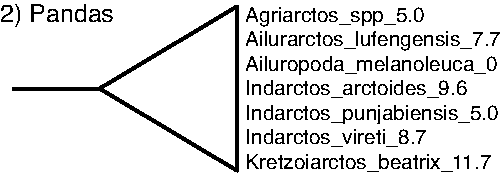
\includegraphics[width=3in]{figures/ts_pandas.pdf}}
\caption{\small The species belonging to the Panda clade.}
\label{figtaxset2}
\end{figure}

%\begin{framed}
%Create a new taxon set for node 2 by clicking the \fbox{\textbf{+}} and label it \cl{2\_Pandas}.
%
%Move all of the taxa listed in this clade (see Figure \ref{figtaxset2}) to the right-hand column and click \mi{OK}.
%
%Back in the \mi{Priors} window, check the box labeled \mi{monophyletic} for node 2.
%\end{framed}

The subfamily Tremarctinae includes only the extant spectacled bear (\textit{Tremarctos ornatus}) and the short-faced bear (\textit{Arctodus simus}), shown in Figure \ref{figtaxset3}. 
The occurrence time of the short-faced bear is only 500,000 years ago since it is known from the Pleistocene.

\begin{figure}[h!]
\centering
\fbox{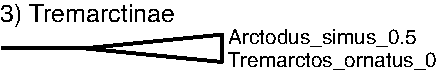
\includegraphics[width=3in]{figures/ts_Tremarctini.pdf}}
\caption{\small The two species in the clade Tremarctinae.}
\label{figtaxset3}
\end{figure}

%\begin{framed}
%Create a new taxon set for node 3 by clicking the \fbox{\textbf{+}} and label it \cl{3\_Tremarctinae}.
%
%Move both species listed in this clade (see Figure \ref{figtaxset3}) to the right-hand column and click \mi{OK}.
%
%Back in the \mi{Priors} window, check the box labeled \mi{monophyletic} for node 3.
%\end{framed}

The subfamily Ursinae comprises all of the species in the genus \textit{Ursus} (including two fossil species) as well as the sun bear (\textit{Helarctos malayanus}) and the sloth bear (\textit{Melursus ursinus}). 
These species are listed in Figure \ref{figtaxset4}.

\begin{figure}[h!]
\centering
\fbox{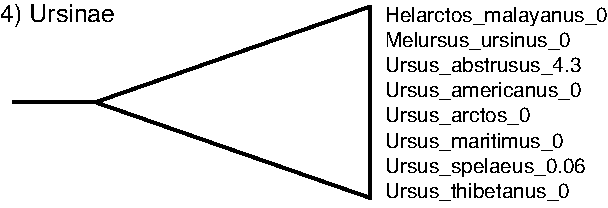
\includegraphics[width=3in]{figures/ts_ursinae.pdf}}
\caption{\small The species belonging to the subfamily Ursinae.}
\label{figtaxset4}
\end{figure}

%\begin{framed}
%Create a new taxon set for node 4 by clicking the \fbox{\textbf{+}} and label it \cl{4\_Ursinae}.
%
%Move all of the taxa listed in this clade (see Figure \ref{figtaxset4}) to the right-hand column and click \mi{OK}.
%
%Back in the \mi{Priors} window, check the box labeled \mi{monophyletic} for node 4.
%\end{framed}

Finally, multiple studies using molecular data have shown that the polar bear (\textit{Ursus maritimus}) and the brown bear (\textit{Ursus arctos}) are closely related.
Furthermore, phylogenetic analyses of ancient DNA from Pleistocene sub-fossils concluded that the cave bear (\textit{Ursus spelaeus}) is closely related to the polar bear and the brown bear (Figure \ref{figtaxset5}).
This taxon set is not included in our \cl{NEXUS} file, so we must define it using BEAUti.


\begin{figure}[h!]
\centering
\fbox{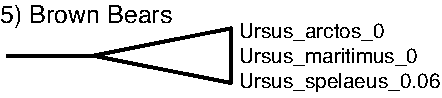
\includegraphics[width=3in]{figures/ts_polar.pdf}}
\caption{\small Three closely related \textit{Ursus} species in the ``Brown Bears'' clade.}
\label{figtaxset5}
\end{figure}

\begin{framed}
Create a new taxon set for node 5 by clicking the \fbox{\textbf{+}} and select \mi{MRCA prior} in the pop-up option box.

Label this taxon set \cl{5\_BrownBears}.

Move all of the taxa listed in this clade (Figure \ref{figtaxset5}) to the right-hand column, click \mi{OK} [Figure \ref{screentaxsetBB}].

Back in the \mi{Priors} window, check the box labeled \mi{monophyletic} for node 5.
\end{framed}

\begin{figure}[h!]
\centering
\fbox{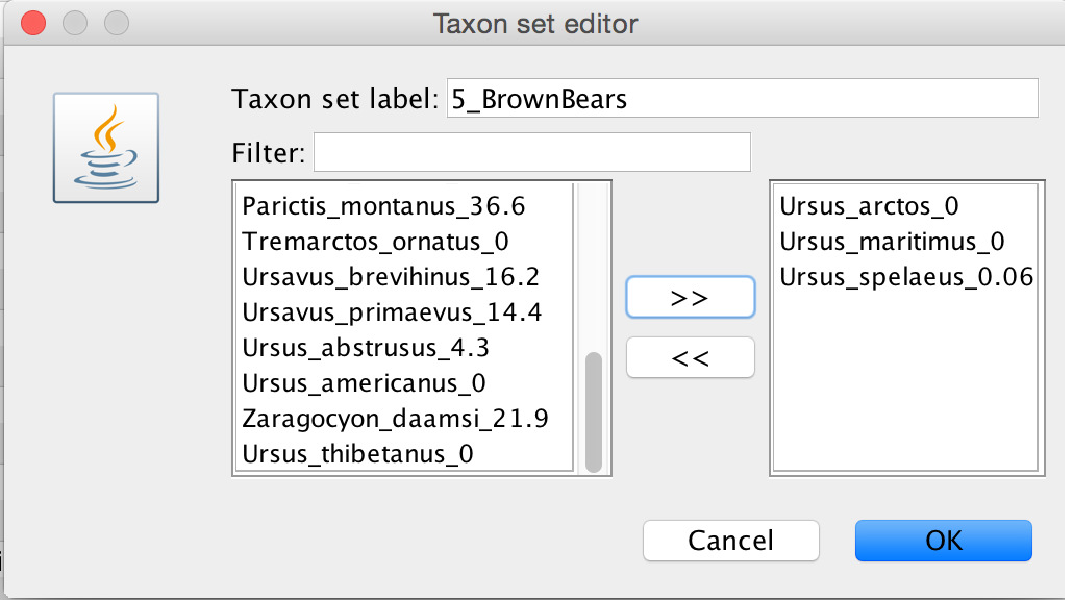
\includegraphics[width=4in]{figures/brown_bears_taxset.pdf}}
\caption{\small The \mi{Taxon set editor} used to create the clade containing the brown bear, polar bear, and cave bear.}
\label{screentaxsetBB}
\end{figure}

At this point, there should be five, monophyletic taxon sets listed in the \mi{Priors} window. 


\bigskip
\subsubsection{Other BEAUti Options}

There are two additional windows that are hidden in BEAUti by default. You can reveal them by selecting \mi{View\textrightarrow View All} from the pull-down menu above. 
This will reveal the \mi{Initialization} and \mi{Operators} panels. 
The \mi{Initialization} options allow you to change the starting values for the various parameters and specify if you want them estimated or fixed.
The \mi{Operators} menu contains a list of the parameters and hyperparameters that will be sampled over the course of the MCMC run. In this window, it is possible to turn off any of the elements listed to fix a given parameter to its starting value. For example, if you would like to estimate divergence times on a fixed tree topology (using a starting tree that you provided), then disable proposals operating on the \cl{Tree}. For this exercise, leave both windows unmodified. 


\bigskip
\subsubsection{Set MCMC Options and Save the XML File}


\begin{framed}
Navigate to the \mi{MCMC} window.
\end{framed}

Now that you have specified all of your data elements, models, priors, and operators, go to the \mi{MCMC} tab to set the length of the Markov chain, sample frequency, and file names. By default, BEAST sets the number of generations to 10,000,000.


\begin{framed}
Since we have a limited amount of time for this exercise, change the \mi{Chain Length} to 2,000,000. (Runtimes may vary depending on your computer, if you have reason to believe that this may take a very long time, then change the run length to something smaller.)
\end{framed}

Next we can set the filenames and output frequency.

\begin{framed}
Reveal the options for the \mi{tracelog} using the $\blacktriangleright$ to the left. 
\end{framed}

The frequency parameters are sampled and logged to file can be altered in the box labeled \mi{Log Every}. In general, this value should be set relative to the length of the chain to avoid generating excessively large output files. If a low value is specified, the output files containing the parameter values and trees will be very large, possibly without gaining much additional information. Conversely, if you specify an exceedingly large sample interval, then you will not get enough information about the posterior distributions of your parameters.

\begin{framed}
Change \mi{Log Every} to \cl{100}. Also specify a name for the log file by changing \mi{File Name} to \cl{bearsDivtime\_FBD.log}.
\end{framed} 

Next, we will specify how the trees are written to file. 
Analyses in BEAST often estimate parameters that are associated with each branch in the tree (i.e, substitution rate).
Additionally, the tree topology and branching times for each MCMC iteration can be written to file.
These parameters are stored in a different file with the trees written in extended Newick format. 
The default name for this file is \cl{\$(tree).trees}. The string ``\cl{\$(tree)}'' indicates the name of the tree we defined in the \mi{Partitions} panel. For this analysis we relabeled this variable: \cl{bearsTree} and our file name will begin with \cl{bearsTree} even if we do not alter the name of this file.
\begin{framed} 
Reveal the options for the \mi{treelog.t:bearsTree} file. Keep the \mi{File Name} \cl{\$(tree).trees} and \mi{Log Every} to \cl{100}.
\end{framed} 

%Note that both files have the digit \cl{1} in the file name. That is because we intend to run this analysis multiple times.
An important part of any MCMC analysis is that multiple, independent runs are executed starting from different initial states for the various parameters.
To do this, one can create multiple files in BEAUti, ensuring that the log and trees files have different names; or you can simply copy the XML file and alter the file names and starting states in a text editor.
Given the time available for this practical, it isn't feasible to run multiple chains, but the output will be provided for you to evaluate this.

\textit{Now we are ready to save the XML file!}

\begin{framed}
In the pull-down menu save the file by going to \mi{File\textrightarrow Save As} and save the file: \cl{bearsDivtime\_FBD.xml}.
\end{framed}


For the last step in BEAUti, create an XML file that will run the analysis by sampling under the prior. 
This means that the MCMC will ignore the information coming from the sequence data and only sample parameters in proportion to their prior probability.
The output files produced from this run will provide a way to visualize the marginal prior distributions on each parameter.

\begin{framed}
Check the box labeled \mi{Sample From Prior} at the bottom of the \mi{MCMC} panel. We will want to change the names of the output files as well, so change the \mi{tracelog -- File Name} to \cl{bearsDivtime\_FBD.prior.log} and the \mi{treelog.t:bearsTree -- File Name} to \cl{bearsDivtime\_FBD.prior.trees}. 

Save these changes by going to \mi{File\textrightarrow Save As} and name the file \cl{bearsDivtime\_FBD.prior.xml}.
\end{framed}

\bigskip
\subsection{Making changes in the XML file} 

BEAUti is a great tool for generating a properly-formatted XML file for many types of BEAST analyses. However, you may encounter errors that require modifying elements in your input file and if you wish to make small to moderate changes to your analysis, altering the input file is far less tedious than generating a new one using BEAUti. Furthermore, BEAST is a rich program and all of the types of analyses, models, and parameters available in the core cannot be specified using BEAUti. Thus, some understanding of the BEAST XML format is essential.

\begin{framed}Open the \cl{bearsDivtime\_FBD.xml} file generated by BEAUti in your text editor and glance over the contents. BEAUti provides many comments describing each of the elements in the file. 
\end{framed}

As you look over the contents of this file, you will notice that the components are specified in an order similar to the steps you took in BEAUti. The XML syntax is very verbose. This feature makes it fairly easy to understand the different elements of the BEAST input file. If you wished to alter your analysis or realized that you misspecified a prior parameter, changing the XML file is far simpler than going through all of the steps in BEAUti again. For example, if you wanted to change the mean of the exponential prior distribution on the mean clock rate (\cl{ucldMean.c}), this can be done easily by altering this value in the XML file (Box 4), though leave this at \cl{10.0} for this exercise. 
\begin{center}
{\tt \scriptsize{\begin{minipage}{6.5in}
\begin{lstlisting}[language=XML]
<prior id="MeanRatePrior.c:bearsClock" name="distribution" x="@ucldMean.c:bearsClock">
    <Exponential id="Exponential.02" name="distr">
        <parameter id="RealParameter.020" estimate="false" name="mean">10.0</parameter>
    </Exponential>
</prior>
\end{lstlisting}
\end{minipage}}}\\\vspace{4mm}
Box 1: BEAST 2 XML syntax for specifying an exponential prior distribution on the mean clock rate. Changing the expected value of this prior is simply done by altering the XML file.\\
\end{center}

Although running multiple, independent analyses is an important part of any Bayesian analysis, BEAST does not do this by default. However, setting this up is trivial once you have a complete XML file in hand and only requires that you make a copy of the input file and alter the names of the output files in the XML (it's also best to change the initial states for all of your parameters, including the starting tree).
\begin{framed}
If you need to return to your analysis specification in BEAUti, you can load your saved XML file when you reopen the program using the \mi{File\textrightarrow Load} menu options.
\end{framed}


\bigskip
\subsection{Running BEAST 2} 

Now you are ready to start your BEAST analysis. 
%BEAST allows you to use the BEAGLE library if you already have it installed. BEAGLE is an application programming interface and library that effectively takes advantage of your computer hardware (CPUs and GPUs) for doing the heavy lifting (likelihood calculation) needed for statistical phylogenetic inference \citep{ayers12}. Particularly, when using BEAGLE's GPU (NVIDIA) implementation, runtimes are significantly shorter. 

\begin{framed}
Execute \cl{bearsDivtime\_FBD.prior.xml} and \cl{bearsDivtime\_FBD.xml} in BEAST. You should see the screen output every 1,000 generations, reporting the likelihood and several other statistics.
\end{framed}

%\exs{Once you have verified that your XML file was properly configured and you see the likelihood update, feel free to kill the run. I have provided the output files for this analysis and you can find them in \cl{divtime\_beast/output*}.}

\bigskip
\subsection{Summarizing the output}

Once the run reaches the end of the chain, you will find three new files in your analysis directory. The MCMC samples of various scalar parameters and statistics are written to the file called \cl{bearsDivtime\_FBD.log}. The tree-state at every sampled iteration is saved to \cl{bearsTree.1.trees}. The tree strings in this file are all annotated in extended Newick format with the substitution rate from the uncorrelated lognormal model at each node. The file called \cl{bearsDivtime\_FBD.xml.states} summarizes the performance of the proposal mechanisms (operators) used in your analysis, providing information about the acceptance rate for each move. Reviewing this file can help identify operators that might need adjustment if their acceptance probabilities are too high. 

The main output files are the \cl{.log} file and \cl{.trees} file. It is not feasible to review the data contained in these files by simply opening them in a spreadsheet program or a tree viewing program. Fortunately, the developers of BEAST have also written general utility programs for summarizing and visualizing posterior samples from Bayesian inference using MCMC. Tracer is a cross-platform, java program for summarizing posterior samples of scaler parameters. This program is necessary for assessing convergence, mixing, and determining an adequate burn-in. Tree topologies, branch rates, and node heights are summarized using the program TreeAnnotator and visualized in FigTree.

\bigskip  
\subsubsection{Tracer}

This section will briefly cover using Tracer and visual inspection of the analysis output for MCMC convergence diagnostics.

\begin{framed}
Open Tracer and import the \cl{bearsDivtime\_FBD.log} file in the \mi{File\textrightarrow Import New Trace File}.
\end{framed}

The fist statistic loaded will be the \mi{posterior}, in the \mi{Estimates} tab, and you can see the list of statistics and variables that you can navigate through and visualize the summaries.
You may notice that items in the \mi{ESS} column are colored red or gold. The MCMC runs you have performed today are far too short to produce adequate posterior estimates of divergence times and substitution model parameters and this is reflected in the ESS values. The ESS is the \textit{effective sample size} of a parameter. The value indicates the number of effectively independent draws from the posterior in the sample. This statistic can help to identify autocorrelation in your samples that might result from poor mixing. It is important that you run your chains long enough and sufficiently sample the stationary distribution so that the ESS values of your parameters are all high (over 200 or so). 
\begin{framed}
Click on a parameter with a low ESS and explore the various windows in Tracer. It is clear that we must run the MCMC chain longer to get good estimates. 
\end{framed}

Provided with the files for this exercise are the output files from analyses run for 50,000,000 iterations. 
The files can be found in the  \cl{output} directory and are all labeled with the file stem: \cl{bearsDivtime\_FBD.*.log} and \cl{bearsDivtime\_FBD.*.trees}.
\begin{framed}
Close \cl{bearsDivtime\_FBD.log} in Tracer using the \fbox{\textbf{-}} button and open \cl{bearsDivtime\_FBD.1.log}, \cl{bearsDivtime\_FBD.2.log} and \cl{bearsDivtime\_FBD.prior.log}.
\end{framed}

These log files are from much longer runs and since we ran two independent, identical analyses, we can compare the log files in Tracer and determine if they have converged on the same stationary distribution. Additionally, analyzing samples from the prior allows you to compare your posterior estimates to the prior distributions used for each parameter. 

\begin{framed}
Select and highlight all three files (\cl{bearsDivtime\_FBD.1.log}, \cl{bearsDivtime\_FBD.2.log} and\\ \cl{bearsDivtime\_FBD.prior.log}) in the \mi{Trace Files} pane (do not include \mi{Combined}). This allows you to compare all three runs simultaneously. Click on the various parameters and view how they differ in their estimates and 95\% credible intervals for those parameters
\end{framed}

The 95\% credible interval is a Bayesian measure of uncertainty that accounts for the data. If we use the 95\% credible interval, this means that the probability the true value of a parameter lies within this interval is 0.95, given our model and data. This measure is often used to approximate the 95\% highest posterior density region (HPD). 
\begin{framed}
Find the parameter \mi{ucldStdev} and compare the estimates of the standard deviation of the uncorrelated log-normal distribution.
\end{framed}

The \mi{ucldStdev} indicates the amount of variation in the substitution rates across branches. Our prior on this parameter is an exponential distribution with $\nu = 2.997$ ($mean = 0.3337$). Thus, there is a considerable amount of prior weight on \mi{ucldStdev} $= 0$. A standard deviation of 0 indicates support for no variation in substitution rates and the presence of a molecular clock. 

\begin{framed}
With \mi{ucldStdev} highlighted for all three runs, go to the \mi{Marginal Density} window, which allows you to compare the marginal posterior densities for each parameter. (By default Tracer gives the kernel density estimate (\mi{KDE}) of the marginal density. You can change this to a \mi{Histogram} using the options at the top of the window.)

Color (or ``colour'') the densities by \mi{Trace File} next to \mi{Colour by} at the bottom of the window (if you do not see this option, increase the size of your Tracer window). You can also add a \mi{Legend} to reveal which density belongs to which run file. [Figure \ref{tracerStdev}]
\end{framed}

%% Look at turnover rate, notice that it's not uniform, that's because this run wasn't completely under the prior since the data coming from the fossil observation times is still being considered.
%Thus the FBD calculates the probability conditional on the times provided, and thus the turnover and diversification will be sampled accordingly.

\begin{figure}[h!]
\centering
%\fbox{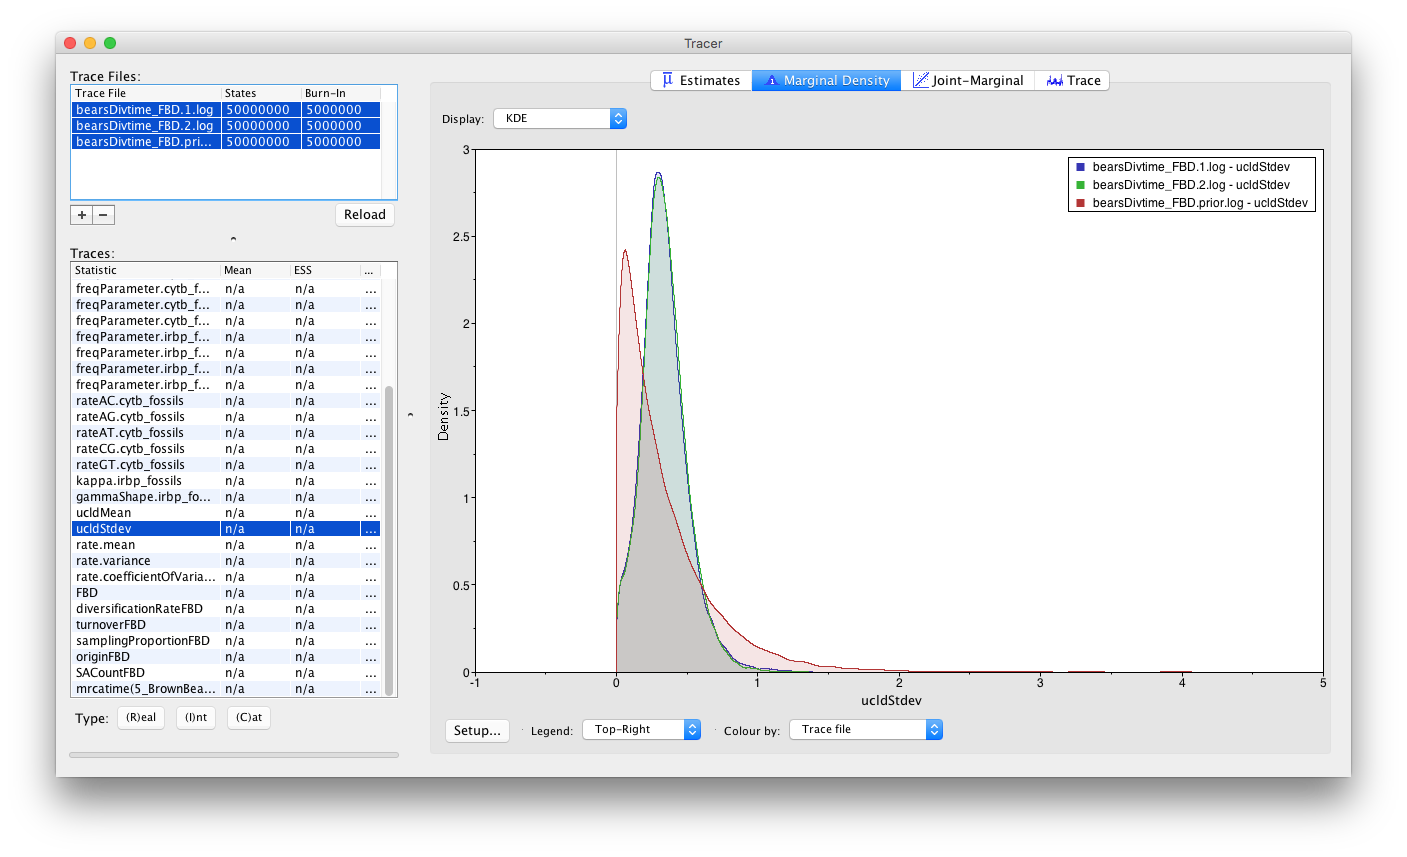
\includegraphics[width=6in]{figures/tracer_image_stdev.png}}
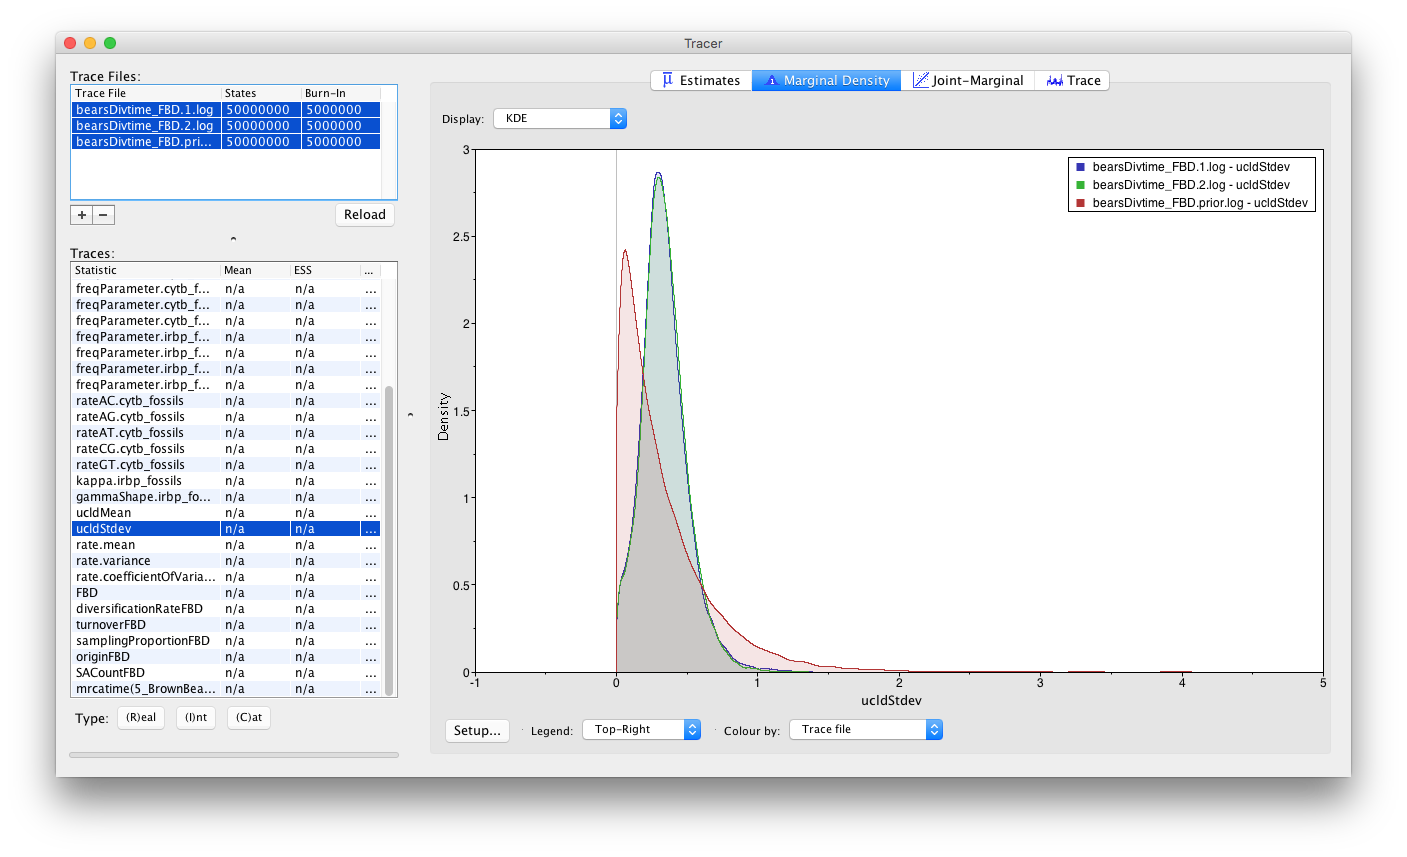
\includegraphics[width=6in]{figures/tracer_image_stdev.png}
\caption{\small Comparing the marginal densities (using the kernel density estimate) of the \mi{ucldStdev} parameter from 2 independent runs (blue and green) and the prior (red) in Tracer.}
\label{tracerStdev}
\end{figure}

The first thing you will notice from this plot is that the marginal densities from each of our analysis runs (\cl{bearsDivtime\_FBD.1.log} and \cl{bearsDivtime\_FBD.2.log}) are nearly identical. If you click through the other sampled parameters, these densities are the same for each one. This indicates that both of our runs have converged on the same stationary distribution. If some of the other parameters might not have mixed well, we may want to run them longer, but we can have good confidence that our runs have sampled the same distribution. 

Second, it is likely for the UCLD rates that the parameters of this model appear to be somewhat sensitive to the priors. 
That is because we have several lineages in our tree without any data since we are using fossils to calibrate under the FBD model. 
For these branches, the clock rate assigned to them is sampled from the prior.
The branches with extant descendants, however have rates that are informed by DNA sequence data.
Because of this implementation, it is difficult to visualize the branch rates and associated parameters from the log files. 
If these parameters are of interest, then it may be necessary to extract the rates associated with the extant branches from the MCMC samples of trees. 
When fossils are used without character data, alternative implementations of the FBD model consider the fossils separately and thus, the branch rates can be summarized for only the extant lineages \citep{heath2013fossilized}.

Next, we will look at the \mi{Marginal Prob Distribution} for the turnover parameter (\mi{turnoverFBD}).
\begin{framed}
Select all trace files for the \mi{turnoverFBD} parameter and go to the \mi{Marginal Density} window.

Color the densities by \mi{Trace file} and add a legend. [Figure \ref{tracerTurnover}]
\end{framed}

\begin{figure}[h!]
\centering
%\fbox{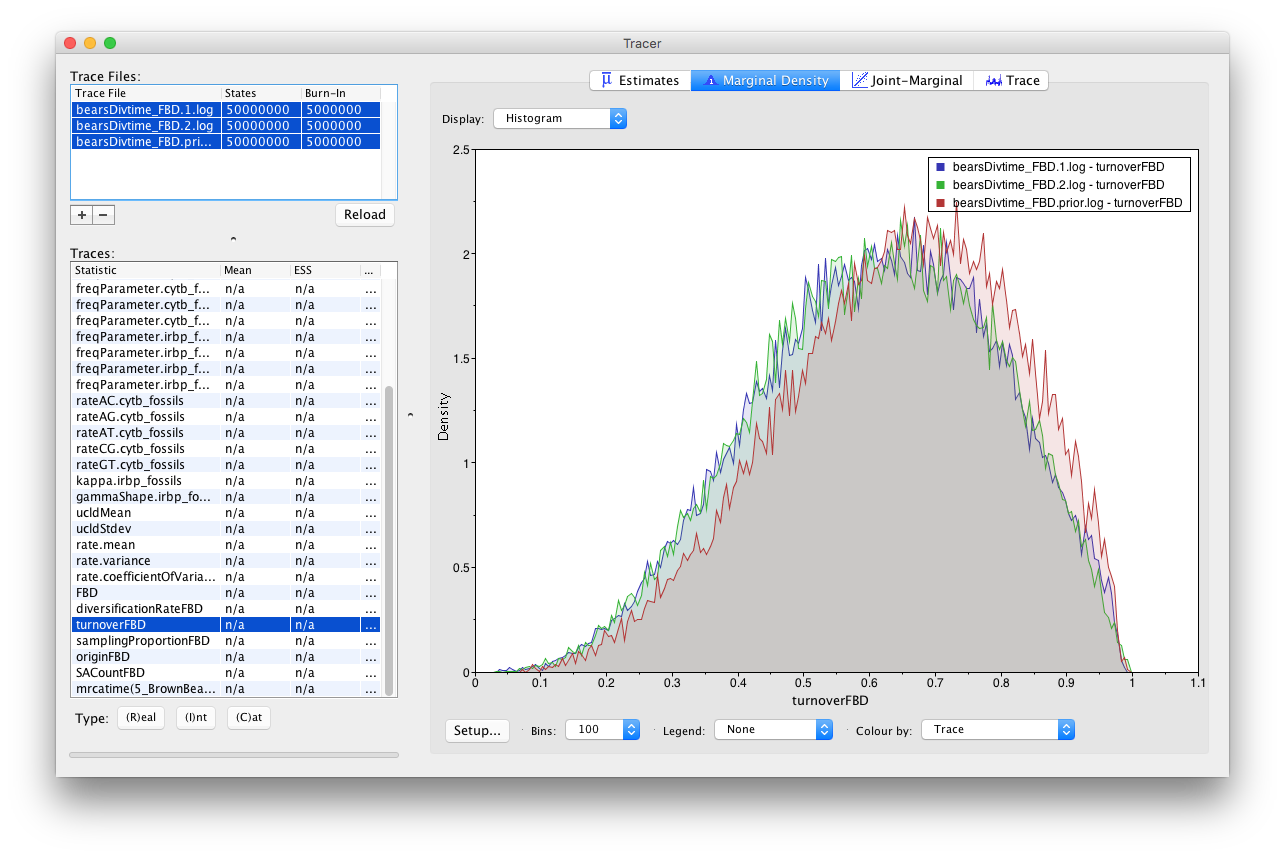
\includegraphics[width=3.4in]{figures/tracer_image_turnover.png}}
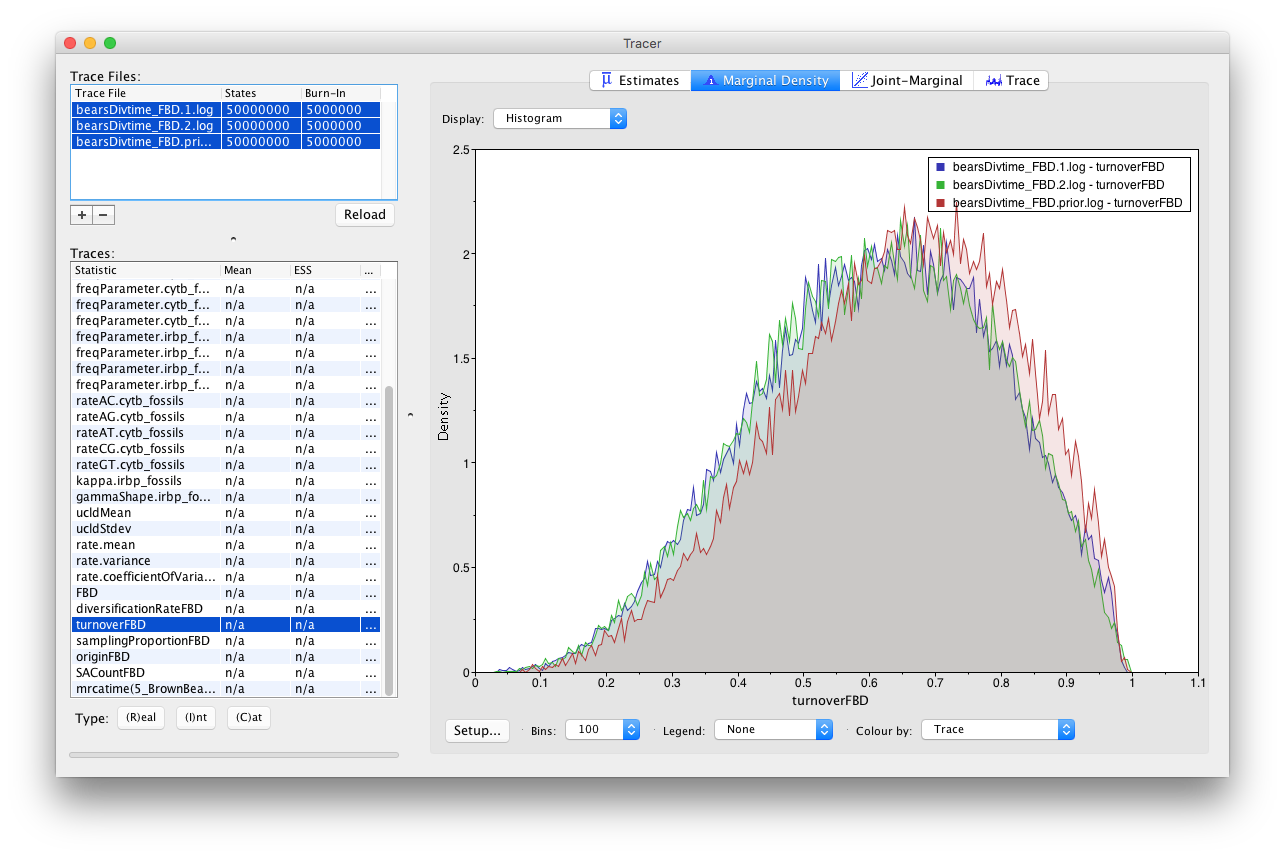
\includegraphics[width=6in]{figures/tracer_image_turnover.png}
\caption{\small Comparing the marginal densities (using the histogram) of the \mi{turnoverFBD} parameter from 2 independent runs (blue and green) and the prior (red) in Tracer.}
\label{tracerTurnover}
\end{figure}

When comparing the MCMC with data to those sampled just under the prior, we can see that this prior and posterior densities are nearly identical. 
Additionally, you may be alarmed that the prior density looks nothing like the Uniform(0,1) prior we applied in BEAUti. 
However, it's important to understand that when specifying \mi{Sample From Prior} in BEAUti we are telling BEAST to ignore the likelihood coming from the \textit{sequence data}, but the MCMC continues to account for the other data---fossil occurrence times---that we have input.
Thus, since we have a good number of fossils, the estimates of turnover, diversification, and the sampling proportion are highly informed by these data.
If we used fewer fossils, the posterior and prior densities would be less congruent because the fossil data are still considered when ``sampling from the prior'' in this case. By contrast, if the information from the fossil occurrence times was ignored when sampling under the prior, then the posterior and prior densities for the FBD parameters would deviate more when many fossils are used.

\begin{framed}
Continue examining the options in Tracer. This program is very, \textit{very} useful for exploring many aspects of your analysis. 
\end{framed}

\bigskip
\subsubsection{Summarizing the Trees in Treeannotator}\label{treeannotatorSec}

After reviewing the trace files from the two independent runs in Tracer and verifying that both runs converged on the posterior distributions and reached stationarity, we can combine the sampled trees into a single tree file and summarize the results.
\begin{framed}
Open the program LogCombiner and set the \mi{File type} to \mi{Tree Files}. Next, import the two tree files in the \cl{output} directory (\cl{bearsDivtime\_FBD.1.trees} and \cl{bearsDivtime\_FBD.2.trees}) using the \fbox{\textbf{+}} button. 

Set a burn-in percentage of 20 for each file, thus discarding the first 20\% of the samples in each tree file. 

Both of these files have 50,000 trees, so it is helpful to thin the tree samples and summarize fewer states (to avoid hitting the maximum memory allotted for this program). Turn on \mi{Resample states at lower frequency} and set this value to 10000.

Click on the \mi{Choose file ...} button to create an output file and run the program. Name the file: \cl{bearsDivtime.combined.trees}.
\end{framed}

Once LogCombiner has terminated, you will have a file containing 40,000 trees which can be summarized using TreeAnnotator. 
TreeAnnotator takes a collection of trees and summarizes them by identifying the topology with the best support, calculating clade posterior probabilities, and calculating 95\% credible intervals for node-specific parameters. All of the node statistics are annotated on the tree topology for each node in the Newick string. 

\begin{framed}
Open the program TreeAnnotator. Since we already discarded a set of burn-in trees when combining the tree files, we can leave \mi{Burnin} set to \cl{0} (though, if TreeAnnotator is taking a long time to load the trees, click on the \mi{Low memory} option at the bottom left and set the burnin to 10--60\% to reduce the number of trees).

For the \mi{Target tree type}, choose \mi{Maximum clade credibility tree}.
\end{framed}
The \mi{Maximum clade credibility tree} is the topology with the highest product of clade posterior probabilities across all nodes. Alternatively, you can select the \mi{Maximum sum of clade credibilities} which sums all of the clade posteriors. Or you can provide a target tree from file.
The \mi{Posterior probability limit} option applies to summaries on a target tree topology and only calculates posteriors for nodes that are above the specified limit. 

\begin{framed}
Choose \mi{Median heights} or \mi{Mean heights} for \mi{Node heights} which will set the node heights of the output tree to equal the median or mean height for each node in the sample of trees.

Choose \cl{bearsDivtime.combined.trees} as your \mi{Input Tree File}. Then name the \mi{Output File:} \cl{bearsDivtime\_FBD.summary.tre} and click \mi{Run}. 
\end{framed}

\bigskip
\subsubsection{Visualizing the Dated Tree}

The tree file produced by TreeAnnotator contains the maximum clade credibility tree and is annotated with summaries of the various parameters.
\begin{framed}
Open \cl{bearsDivtime\_FBD.summary.tre} in your text editor. The tree is written in NEXUS format. Look at the tree string and notice the annotation. Each node in the tree is labeled with comments using the \cl{[\&parameter\_name=\textless value\textgreater ]} format.
\end{framed}

The summary tree and it's annotations can be visualized in the program FigTree.
\begin{framed}
Execute FigTree and open the file \cl{bearsDivtime\_FBD.summary.tre}.

Explore the options for viewing different summary statistics on the tree.
\end{framed}

The tree you are viewing in FigTree has several fossil taxa with zero-length branches, e.g., \textit{Parictis montanus} and \textit{Ursus abstrusus}. 
These branches actually indicate fossil taxa with a significant probability of representing a sampled ancestor. 
However, it is difficult to represent this in typical tree-viewing programs. 
A tree with sampled ancestors properly represented will have two-degree nodes --- i.e., a node with only one descendant. 
The web-based tree viewer \href{http://icytree.org/}{IcyTree} \citep{Vaughan2017} is capable of plotting such trees from BEAST2 analyses (Figure \ref{icyTree}). 

\begin{figure}[h!]
\centering
\fbox{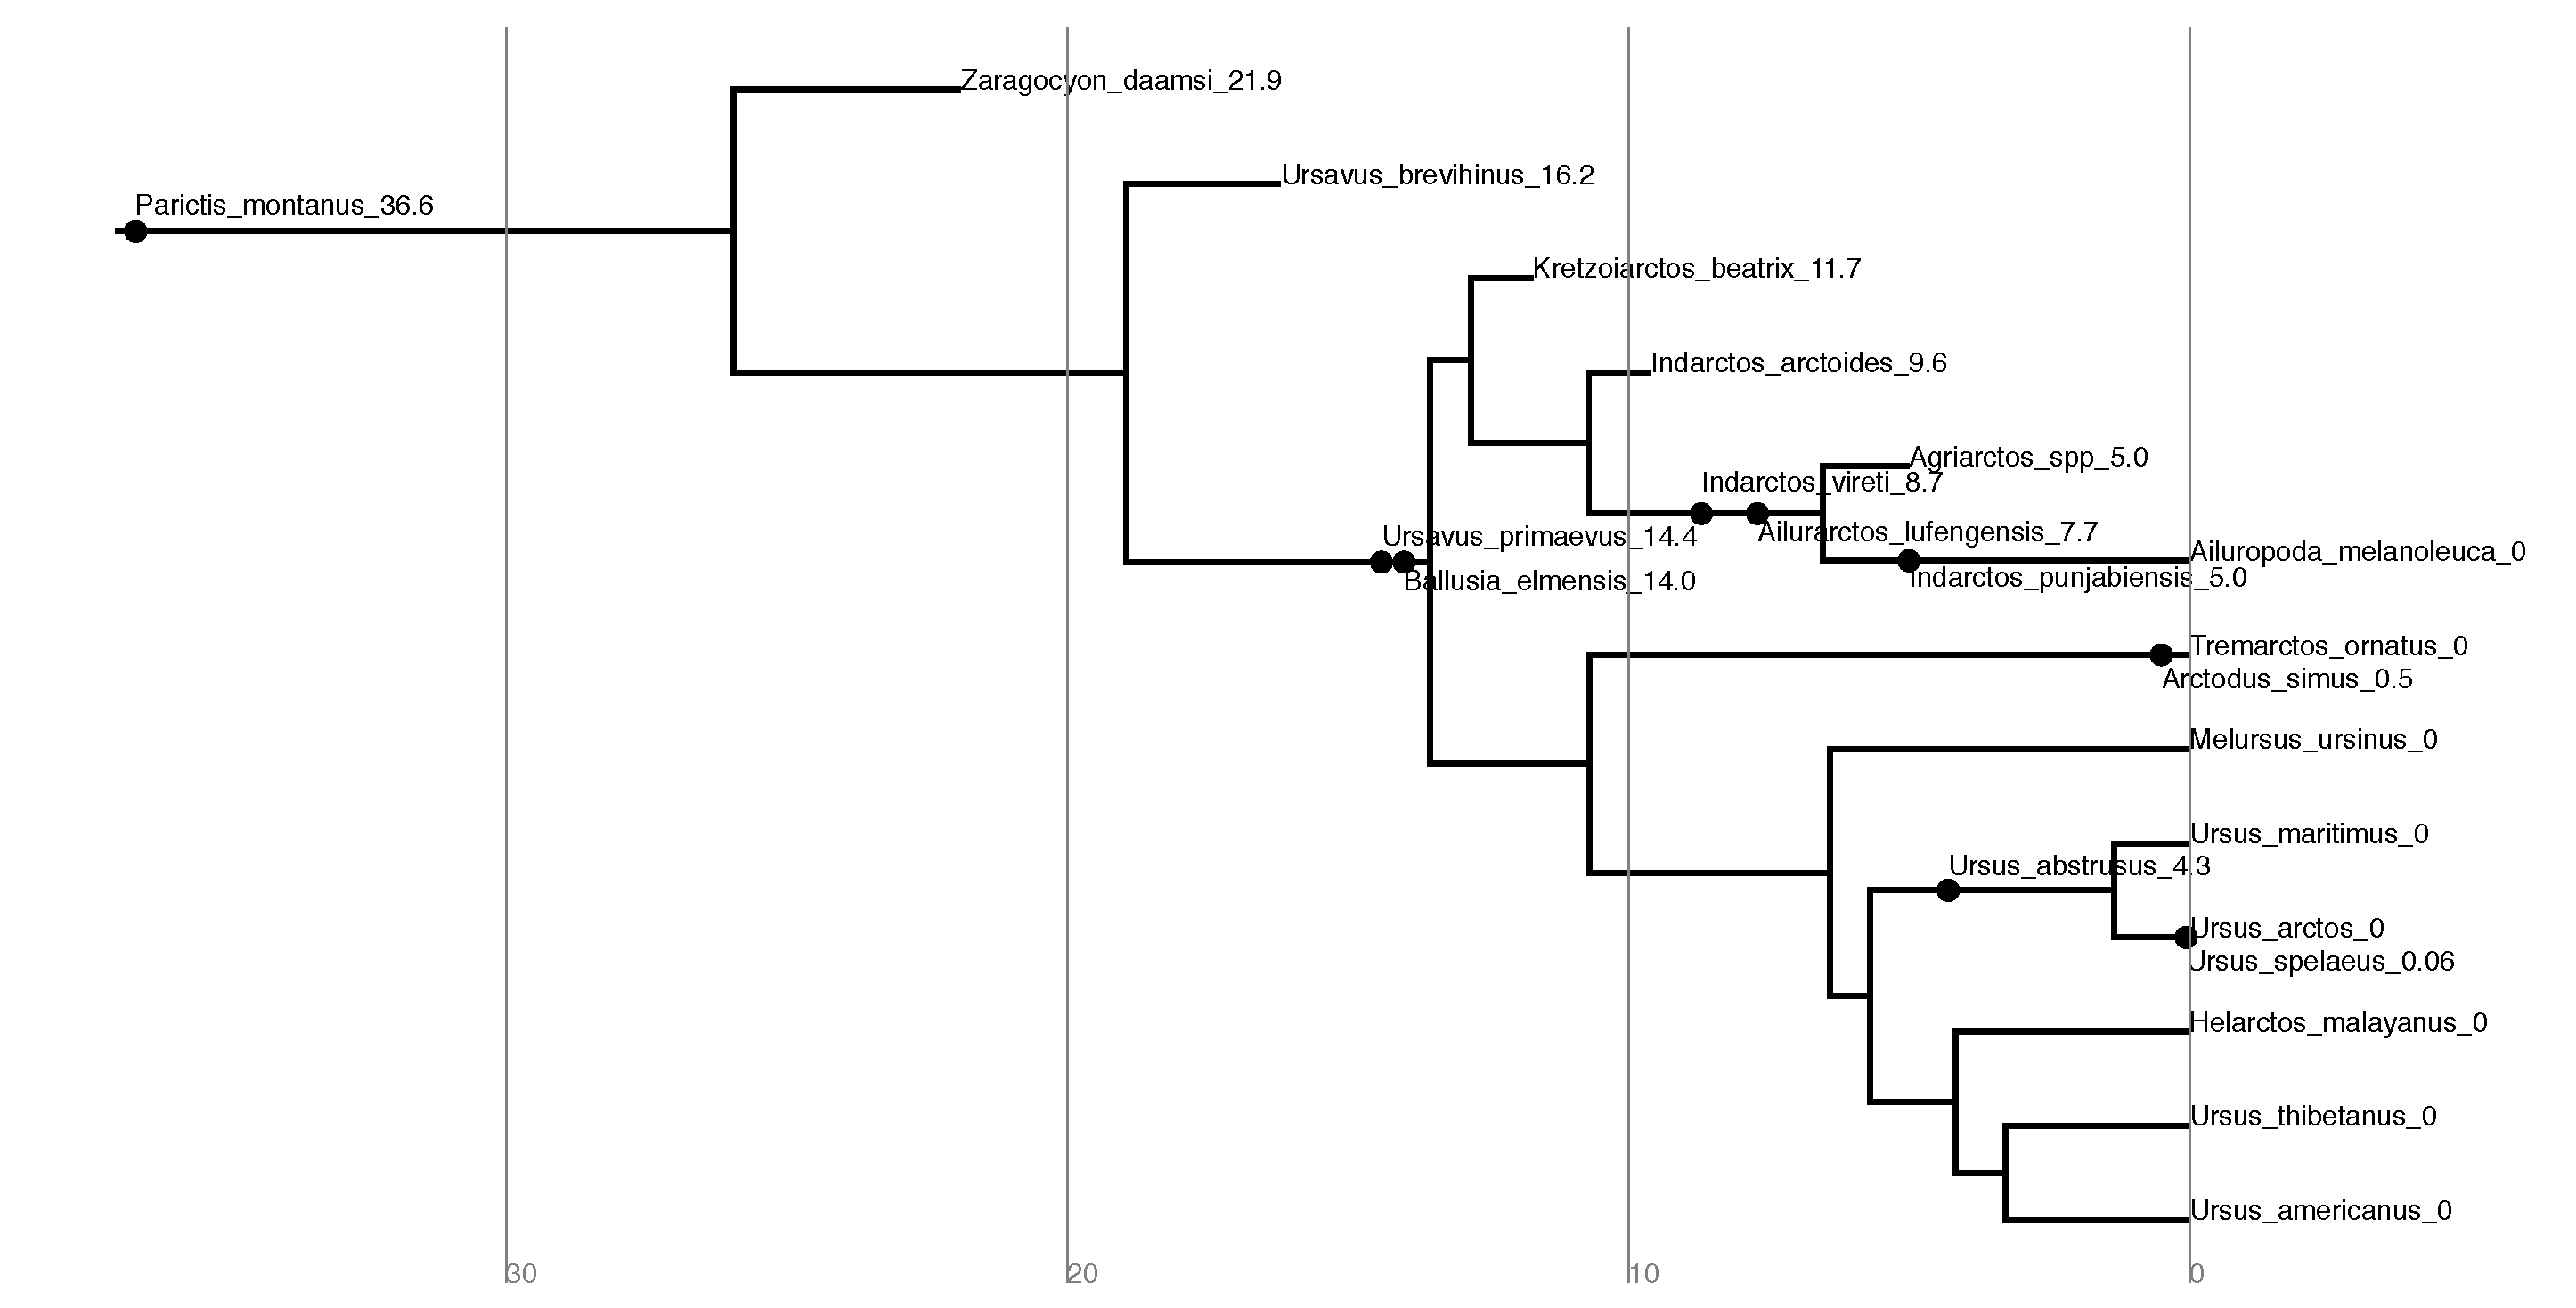
\includegraphics[width=\textwidth]{figures/bearsDivtime_icytree.pdf}}
\caption{\small A sampled-ancestor tree exported from \href{http://tgvaughan.github.io/icytree/icytree.html}{IcyTree}. The sampled-ancestor nodes are revealed by selecting the \mi{Mark singletons} and \mi{Internal node text} set to \mi{Label}. The tree was exported to a SVG file and minor manipulations were conducted in a vector graphics editing program (Inkscape or Adobe Illustrator).}
\label{icyTree}
\end{figure}

Although the tree in Figure \ref{icyTree} (and also Figure \ref{figgeoscale}) looks awesome, the topology can be misleading for this particular analysis. 
Because we did not provide character data for our 14 fossil taxa, the tree topology does not adequately illustrate the degree of uncertainty in the phylogenetic relationships of the fossil lineages.
\textbf{Without morphological data, the fossil lineages can attach to any lineage on the tree that is consistent with the monophyletic clades we specified and the fossil occurrence times with equal probability. 
Thus, the relationships shown here are not reliable as phylogenetic inferences.} 
However, if we provided morphological character data for these fossils, then many would consider this tree to be an adequate summary our MCMC sample of trees. 

Since the fossil taxa were used in this analysis to only inform the fossilized birth-death model, we can prune off all of the fossil lineages and plot the tree with the geological time scale.
BEAUti has a few accessory applications that are for post-processing files from certain types of analyses. 
The first one we will use is called \mi{FullToExtantTreeConverter}.
This program can be used to prune the fossil lineages off of the MCMC sample of trees (in file \cl{bearsDivtime\_FBD.combined.trees}), then use TreeAnnotator to summarize the extant-only trees. 

\begin{framed}
Open BEAUti and launch the accessory apps in the file menu: \mi{File\textrightarrow Launch Apps}.

This will open a window with a few applications, launch \mi{FullToExtantTreeConverter}.

In the file specification window for \mi{Trees} provide the file called \cl{bearsDivtime\_FBD.combined.trees}.

And give the \mi{Output} file the name \cl{bearsDivtime\_FBD.extant.trees}. %[Figure \ref{fullConverterScreen}]

%\end{framed}
%
%\begin{figure}[h!]
%\centering
%\fbox{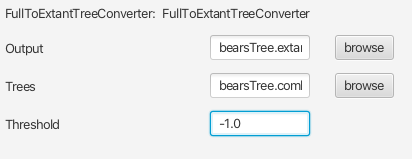
\includegraphics[width=3in]{figures/full_to_extant_converter.pdf}}
%\caption{\small The options for \mi{FullToExtantTreeConverter}.}
%\label{fullConverterScreen}
%\end{figure}
%
%\begin{framed}
Run TreeAnnotator on the file called \cl{bearsDivtime\_FBD.extant.trees}, selecting the same options as you did for the file with complete trees (see Section \ref{treeannotatorSec}). 

Name the summary tree file \cl{bearsDivtime\_FBD.extant\_summary.tre}
\end{framed}

When the fossil lineages are removed, much of the information about the history of this group is lost (Figure \ref{figgeoscaleext}). 
However, alternative approaches for summarizing fossilized birth-death trees are currently under development.
\begin{figure}[h!]
\centering
\fbox{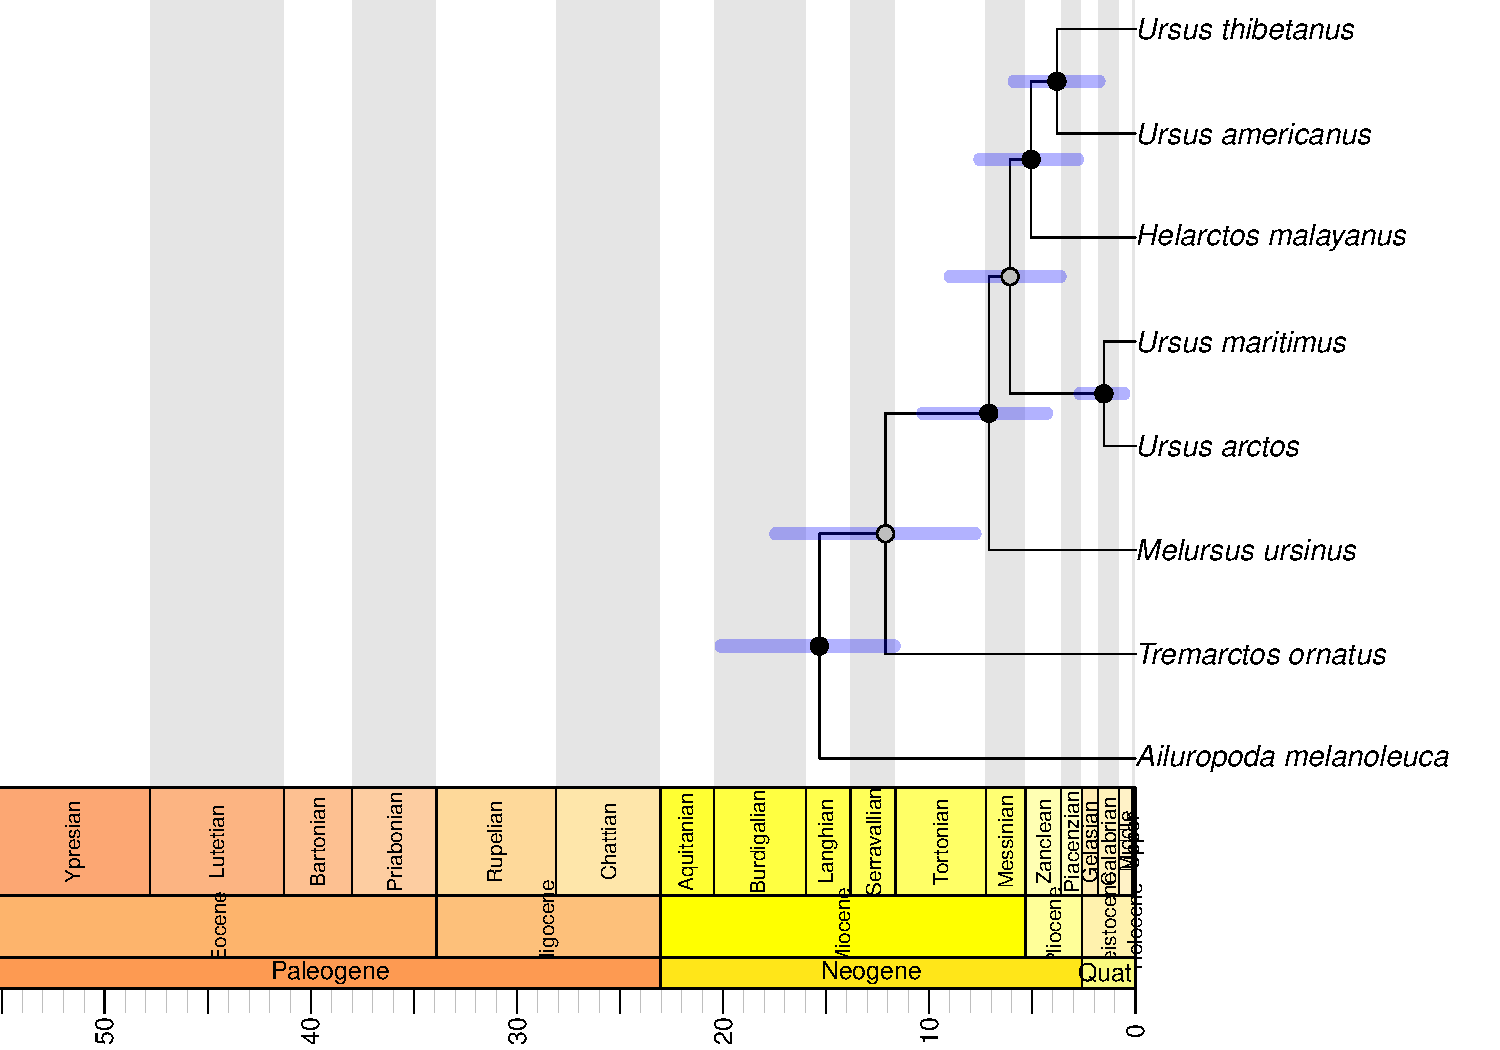
\includegraphics[width=5.5in]{figures/geoscaled_bears_ext.pdf}}
\caption{\small The maximum clade credibility tree of \textit{extant} bears summarized by TreeAnnotator and plotted against stratigraphy using the \cl{strap} package in \cl{R} (see how to do this in Section \ref{section-r-treeviz} below). 
The internal nodes of the tree are indicated with circles, where circles mark nodes with posterior probability: $\newmoon \geq 0.95$, $0.95>$ \gcirc $\geq 0.75$, $0.75 > \fullmoon$. The 95\% credible intervals for node ages are shown with transparent blue bars.}
\label{figgeoscaleext}
\end{figure}

\bigskip
\subsubsection{Analysis of Sampled Ancestors}

Another tool that is available in the BEAUti accessory applications, is \mi{SampledAncestorTreeAnalyser}. If you run this app from the \mi{Launch apps} menu in BEAUti on the file with all the MCMC samples of the complete tree (\cl{bearsDivtime\_FBD.combined.trees}), you will get a report that summarizes the clades/nodes in the sampled ancestor tree. 
In particular, it gives a quantitative representation of ``ancestral-ness'' in the posterior sample of trees. 
This is represented by listing how often a particular node is ancestral to other nodes.
The summary is generated and automatically opens in your web browser.

%It is important to note, however, that the summary approaches for sampled-ancestor trees (for producing a summary topology and the sampled ancestor analyzer) are still under development.

\bigskip
\subsubsection{Visualizing the Dated Tree on a Geological Time Scale$^*$}\label{section-r-treeviz}

$^*$Note that some of the \cl{R} packages required for this section may be difficult to download.

FigTree and IcyTree are great tree-viewing programs and also allow you to produce publication-quality tree figures. 
However, viewing a dated phylogenetic tree with a unit-less timescale is not as meaningful as plotting the tree with a geological (stratigraphic) time scale. 
The \cl{R} package \href{http://cran.r-project.org/web/packages/strap/index.html}{\cl{strap}} \citep{bell2014strap} offers several nice functions for visualizing time-calibrated phylogenies in the context of the rock record.


\descriptionhead{Install R Packages for Viewing and Plotting Trees}

For this exercise we will use some \cl{R} packages to visualize the summary tree with a geological timescale.
If you do not already have \cl{R} installed, please download the current version: \href{http://www.r-project.org/}{http://www.r-project.org}

\dhead{strap} 
Viewing dated phylogenies with an arbitrary time-scale removes the context of geological time and the fossil record from the analysis. 
The package \cl{strap} in \cl{R} provides a set of functions to plot trees and stratigraphic information against geologic time, with scales provided by different sources including the International Commission on Stratigraphy \citep{bell2014strap}.
A detailed tutorial for using the functions in \cl{strap} is available here: \href{http://datadryad.org/resource/doi:10.5061/dryad.4k078}{http://datadryad.org/resource/doi:10.5061/dryad.4k078}.
To install \cl{strap}, execute the following command in \cl{R}:
\begin{lstlisting}[language=R]
> install.packages("strap",dependencies=TRUE)
\end{lstlisting}

\dhead{phytools} 
In \cl{R}, there are many packages available for performing phylogenetic comparative methods, among them \href{http://www.phytools.org}{\cl{phytools}} is one of the richest, providing functions for a wide range of different analyses and for visualizing evolutionary processes in the context of phylogenetic relationships \citep{revell2012phytools}.
To install \cl{phytools} in \cl{R}, execute the following command:
\begin{lstlisting}[language=R]
> install.packages("phytools",dependencies=TRUE)
\end{lstlisting}


\dhead{phyloch} 
The trees sampled by the MCMC in BEAST contain valuable information about the sampled divergence times and branch rates. 
Additionally, the summary trees produced by the BEAST accessory program TreeAnnotator have information about the 95\% credible intervals for the ages and rates. The package \cl{phyloch} provides functions for reading in data files written by BEAST and its accessory programs \citep{heibl2008phyloch}. 
This package, however, is not available for download from CRAN. Instead, it is hosted on the developer's \href{http://www.christophheibl.de/Rpackages.html}{website}. 
To install the \cl{phyloch} package in \cl{R}, first load the \cl{devtools} package and install \cl{phyloch} directly from the URL:
\begin{lstlisting}[language=R]
> library("devtools")
> install_url("http://www.christophheibl.de/phyloch_1.5-5.tgz")
\end{lstlisting}



\descriptionhead{Plot the Tree in \cl{R}}

\begin{framed}
Begin by opening an \cl{R} instance and load the \cl{strap} package.

\begin{lstlisting}[language=R]
> library("strap")
\end{lstlisting}

Now we can read in the tree using the \cl{ape} function \cl{read.nexus()} (note that you might have to type in the whole file path to your tree).
\begin{lstlisting}[language=R]
> tree <- read.nexus("bearsDivtime.summary.tre")
\end{lstlisting}

In order to use the \cl{geoscalePhylo()} function of \cl{strap}, we have to set a value for the variable \cl{tree\$root.time}, which is the age of the root. We can compute this from the tree using the \cl{dist.nodes()} function from \cl{ape}:
\begin{lstlisting}[language=R]
> tree$root.time <- max(dist.nodes(tree))
\end{lstlisting}

Now plot the tree:
\begin{lstlisting}[language=R]
> geoscalePhylo(tree=ladderize(tree,right=FALSE),label.offset=0)
\end{lstlisting}
\end{framed}
You will notice that the plotted figure might need some work to make it easier to read taxon labels, etc. 
Additionally, we don't get the node bars or other summary statistics for our tree. 
If we wish to plot these values, then we need to do a bit more in \cl{R}. 
With additional packages and functions, we can produce a summary tree that includes the credible intervals on the node ages (only for nodes in the extant tree, the origin time, and symbols representing the posterior probabilities of the tree bipartitions).
This tree is shown in Figure \ref{figgeoscale} and the \cl{R} syntax for producing this figure is provided in the \cl{output} directory in the download files (\cl{plot\_geoscaled\_tree.R}).



\begin{figure}[h!]
\centering
\fbox{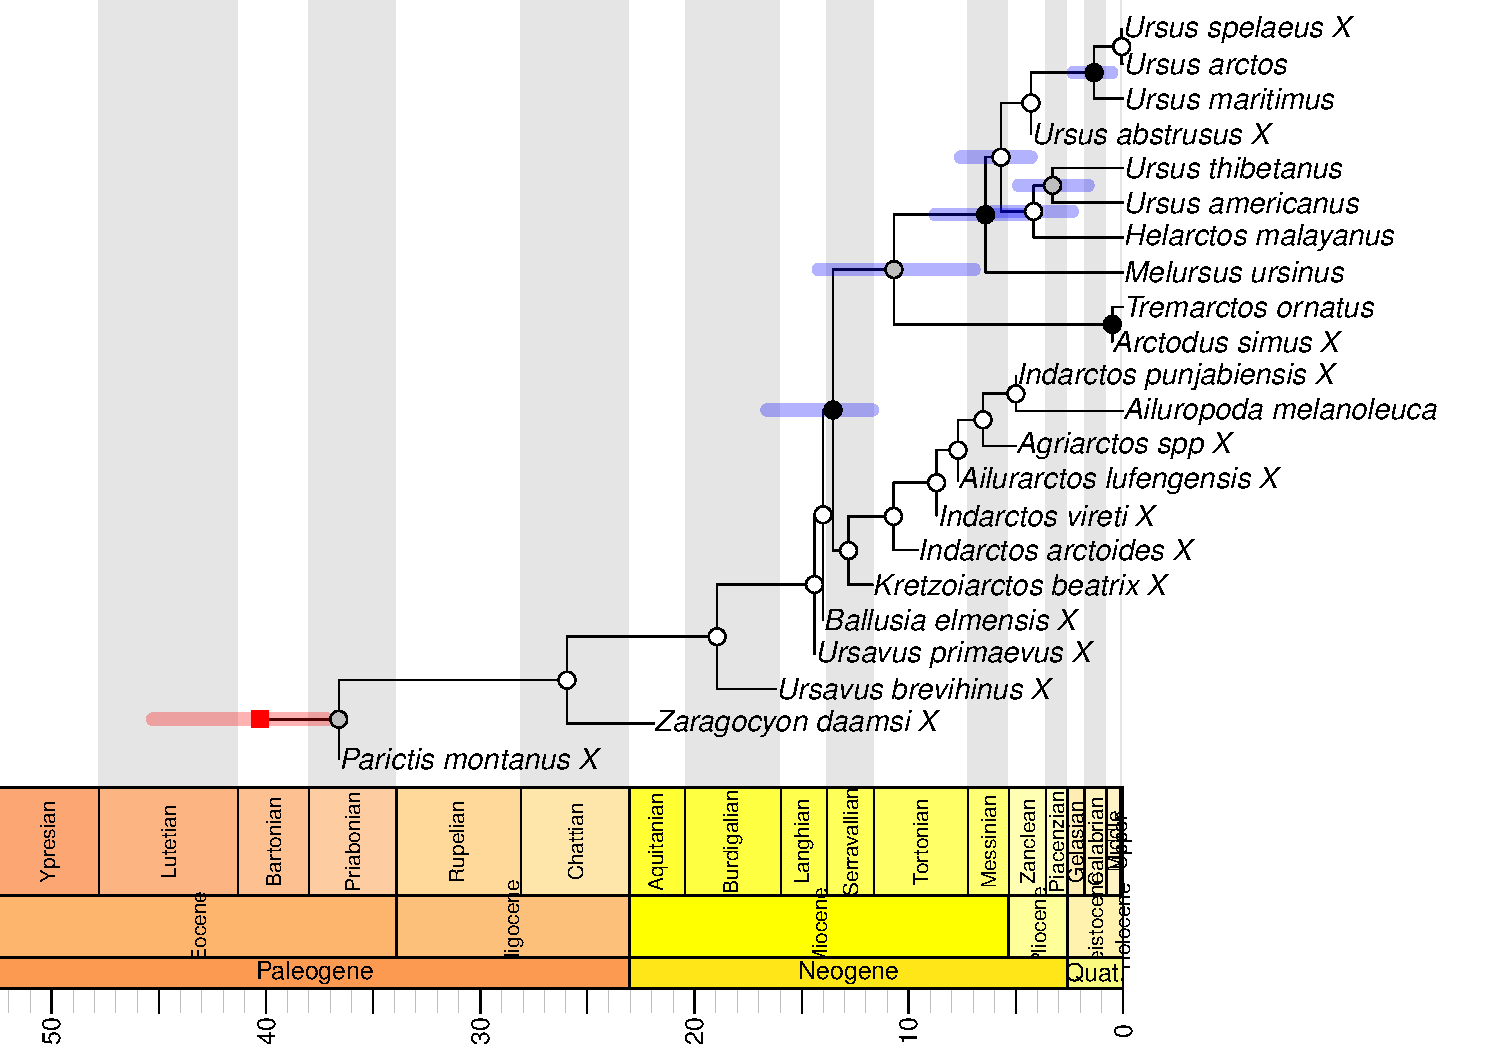
\includegraphics[width=6.2in]{figures/geoscaled_bears.pdf}}
\caption{\small The maximum clade credibility tree summarized by TreeAnnotator and plotted with a geological time scale using the \cl{strap} package in \cl{R}. The fossil taxa are all indicated with an \textit{X} in the taxon names. The {\textcolor{red}{$\blacksquare$}} represents the mean origin time. The remaining internal nodes of the tree are indicated with circles, where circles mark nodes with posterior probability: $\newmoon \geq 0.95$, $0.95>$ \gcirc $\geq 0.75$, $0.75 > \fullmoon$. The 95\% credible intervals for node ages are shown with transparent bars, for only nodes that are represented in the \textit{extant} tree. (The \cl{R} code to produce this figure is in the \cl{output} folder in the file \cl{plot\_geoscaled\_tree.R}.)}
\label{figgeoscale}
\end{figure}

%%%%%
\bigskip
\section{Useful Links}

\begin{itemize}
\item Taming the BEAST -- tutorials and workshops for learning BEAST 2: \href{https://taming-the-beast.github.io/}{https://taming-the-beast.github.io}
\item BEAST 2 website and documentation: \href{http://www.beast2.org/}{http://www.beast2.org} 
\item BEAST 1 website and documentation: \href{http://beast.bio.ed.ac.uk}{http://beast.bio.ed.ac.uk} 
\item Join the BEAST user discussion: \href{http://groups.google.com/group/beast-users}{http://groups.google.com/group/beast-users} 
\item RevBayes: \href{https://github.com/revbayes/code}{https://github.com/revbayes/code} 
\item DPPDiv: \href{https://github.com/trayc7/FDPPDIV}{https://github.com/trayc7/FDPPDIV} 
\item PhyloBayes: \href{http://megasun.bch.umontreal.ca/People/lartillot/www/index.htm}{www.phylobayes.org/} 
\item multidivtime: \href{http://statgen.ncsu.edu/thorne/multidivtime.html}{http://statgen.ncsu.edu/thorne/multidivtime.html} 
\item MCMCtree (PAML): \href{http://abacus.gene.ucl.ac.uk/software/paml.html}{http://abacus.gene.ucl.ac.uk/software/paml.html}
\item BEAGLE: \href{http://code.google.com/p/beagle-lib/}{http://code.google.com/p/beagle-lib/} 
\item A list of programs: \href{http://evolution.genetics.washington.edu/phylip/software.html}{http://evolution.genetics.washington.edu/phylip/software.html} 
\item The Paleobiology Database: \href{http://www.paleodb.org}{http://www.paleodb.org} 
\item The Fossil Calibration Database: \href{http://fossilcalibrations.org}{http://fossilcalibrations.org}
\end{itemize}


%\clearpage

\bigskip

%%%%%%%%%%%%%%%%%%%%%%%
% Tutorial disclaimer %
%%%%%%%%%%%%%%%%%%%%%%%
% Please do not change the license
% Add the author names and relevant links
% Add any other aknowledgments here
\href{http://creativecommons.org/licenses/by/4.0/}{
\includegraphics[scale=0.8]{figures/ccby.pdf}} This tutorial was written by \href{http://phyloworks.org/}{Tracy Heath} (with helpful contributions from Alexandra Gavryushkina, Rachel Warnock, and members the \href{https://taming-the-beast.github.io/}{Taming the BEAST} team) for workshops on applied phylogenetics and molecular evolution and is licensed under a \href{http://creativecommons.org/licenses/by/4.0/}{Creative Commons Attribution 4.0 International License}. 


%%%%%%%%%%%%%%%%%%%%
% Do NOT edit this %
%%%%%%%%%%%%%%%%%%%%
Version dated: \today



%\newpage

%%%%%%%%%%%%%%%%
%  REFERENCES  %
%%%%%%%%%%%%%%%%

\printbibliography[heading=relevref]


\end{document}